\documentclass{report}

\usepackage[textwidth=16cm, textheight=24cm]{geometry}
% Packages for special characters and symbols
\usepackage[utf8]{inputenc}
\usepackage[T1]{fontenc}
\usepackage{amsmath, amssymb, amsthm}

% Package for hyperlinks
\usepackage{hyperref}

% Package for graphics
\usepackage{graphicx}
\usepackage{float}
\usepackage{listings}
\usepackage{dirtree}

% Package for better tables
\usepackage{booktabs}
\usepackage{xepersian}

% \setlatintextfont{Times New Roman}
% \settextfont{Yas.ttf}
\settextfont[
BoldFont=Yas Bd.TTF]{Yas.TTF}
% Set the title, author, and date
\title{گزارش پروژه دوم علوم اعصاب محاسباتی}
\author{امیرحسین انتظاری}
\date{\today}

% Begin document
\begin{document}

% Create the title
\maketitle
\newpage
% Create a table of contents
\tableofcontents
% Separate the table of contents from the next content with a new page
% \clearpage

\newgeometry{textwidth=15cm,textheight=22cm}
    \begin{abstract}
        هدف از این پروژه، پیاده سازی سیناپس و جمعیت نورونی، و همچنین بررسی رفتار های آن ها می باشد. در این پروژه ابتدا ساز و کار سیناپسی را با استفاده از تابع دلتای دیراک 
        \footnote{\lr{Dirac delta function}}
        پیاده سازی میکنیم، سپس سه الگوی ارتباطی بین نورون ها را پیاده سازی کرده و با انجام آزمایش های مناسب ویژگی های هر یک را بررسی میکنیم. سپس این الگو های ارتباطی را بین جمعیت های نورونی مختلف قرار داده و آن ها را بررسی میکنیم. در نهایت نیز سه جمعیت نورونی به همراه سیناپس های آن ها درست کرده و و تاثیر آن ها بر یک دیگر را مشاهده می کنیم.
    \end{abstract}
\restoregeometry

\documentclass{report}

\usepackage[textwidth=16cm, textheight=24cm]{geometry}
% Packages for special characters and symbols
\usepackage[utf8]{inputenc}
\usepackage[T1]{fontenc}
\usepackage{amsmath, amssymb, amsthm}

% Package for hyperlinks
\usepackage{hyperref}

% Package for graphics
\usepackage{graphicx}
\usepackage{float}
\usepackage{listings}
\usepackage{dirtree}

% Package for better tables
\usepackage{booktabs}
\usepackage{xepersian}

% \setlatintextfont{Times New Roman}
% \settextfont{Yas.ttf}
\settextfont[
BoldFont=Yas Bd.TTF]{Yas.TTF}
% Set the title, author, and date
\title{گزارش پروژه اول علوم اعصاب محاسباتی}
\author{امیرحسین انتظاری}
\date{\today}

% Begin document
\begin{document}

% Create the title
\maketitle
\newpage
% Create a table of contents
\tableofcontents
% Separate the table of contents from the next content with a new page
% \clearpage

\newgeometry{textwidth=15cm,textheight=22cm}
    \begin{abstract}
        هدف از این پروژه، پیاده سازی سیناپس و جمعیت نورونی، و همچنین بررسی رفتار های آن ها می باشد. در این پروژه ابتدا ساز و کار سیناپسی را با استفاده از تابع دلتای دیراک 
        \footnote{\lr{Dirac delta function}}
        پیاده سازی میکنیم، سپس سه الگوی ارتباطی بین نورون ها را پیاده سازی کرده و با انجام آزمایش های مناسب ویژگی های هر یک را بررسی میکنیم. سپس این الگو های ارتباطی را بین جمعیت های نورونی مختلف قرار داده و آن ها را بررسی میکنیم. در نهایت نیز سه جمعیت نورونی به همراه سیناپس های آن ها درست کرده و و تاثیر آن ها بر یک دیگر را مشاهده می کنیم.
    \end{abstract}
\restoregeometry

\newpage
\section{پیاده سازی ساز و کار سیناپس}
    در این بخش، میخواهیم ساز و کار سیناپس را با استفاده از تابع دلتای دیراک
    \footnote{\lr{Delta Dirac function}}
    پیاده سازی کنیم. جزئیات پیاده سازی در فایل های کد آماده است و فقط در اینجا به نحوه پیاده سازی و همچنین آزمایش آن با یک و دو جمعیت نورونی می پردازیم.

    طبق لینک داده شده، در تجزیه و تحلیل ریاضی، تابع دلتای دیراک
    (یا توزیع $\delta$)، 
    همچنین به عنوان تکانه واحد شناخته می شود، یک تابع تعمیم یافته بر روی اعداد واقعی است که مقدار آن در همه جا صفر است به جز صفر، و انتگرال آن در کل محور حقیقی. برابر یک است.
    \footnote{\href{https://en.wikipedia.org/wiki/Dirac\_delta\_function}{ویکی پدیا}}

    از این رو برای پیاده سازی آن به این صورت عمل میکنیم که ابتدا یک ماتریس به نام 
    $W$ 
    به ابعاد تعداد نورون های پیش سیناپسی
    ($m$)
    در تعداد نورون های پس سیناپسی
    ($n$) 
    ایجاد میکنیم که ماتریس 
    \textbf{وزن}
    های سیناپس ما را تشکیل می دهد.
    ($W_{m\times n}$)
    در هر تکرار
    \footnote{iteration}
    از شبیه سازی، اندیس نورون های پیش سیناپسی که در تکرار قبلی ضربه 
    \footnote{spike}
    زده اند را در یک متغیر مانند 
    \texttt{pre\_spike}
    ذخیره کرده، و از ماتریس وزن ها
    ($W$)
    سطر هایی که ضربه زده اند را جدا کرده و سپس برای هر یک از نورون های پیش سیناپسی و اندیس متناظر، مجموع این وزن ها را حساب کرده و به عنوان جریان سیناپسی ورودی آن نورون در نظر میگیریم و در متغیری مانند 
    \texttt{sg.I}
    ذخیره میکنیم. حال باید این جریان را به جریان نورون های پس سیناپسی اضافه کنیم، اینکار میتواند به راحتی توسط یک رفتار
    \footnote{Behavior}
    به نام دندرایت پیاده سازی شود که در هر تکرار، جریان سیناپسی را به علاوه جریان ورودی نورون می کند:
    \begin{equation}
        I_{ng}(t) = I_{sg}(t-1) + I_{sg}(t)
    \end{equation}

    حال به بررسی رفتار یک یا دو جمعیت نورونی، با پارامتر های مختلف می پردازیم. در این قسمت فقط الگوی ارتباط کامل را بررسی میکنیم و بررسی دقیق تر ۳ الگو را به بخش دوم پروژه واگذار میکنیم.
    \subsection{بررسی رفتار درون یک جمعیت نورونی}
        \subsubsection*{جمعیت نورونی بدون سیناپس}
        برای درک بهتر ساز و کار سیناپس ها، بهتر است ابتدا تاثیر آن را درون یک جمعیت نورونی به تنهایی بررسی کنیم. از این رو اول رفتار یک جمعیت را بدون حضور سیناپس و سپس در حضور سیناپس، بعد گذشت چند تکرار مشاهده میکنیم. 
        همانطور که در شکل 
        \ref{fig:part1-simple-ng}
        مشاهده می کنید، هنگامی که یک جریان ثابت به یک گروه نورونی یکسان وارد می شود، زمان ضربه زدن تمامی نورون ها در یک لحظه اتفاق میوفتد. دلیل این رفتار بدیهی است و بخاطر این است که از آنجا که نورون ها مقادیر یکسانی در هنگام شروع دارند و همچنین جریان یکسانی دریافت می کنند، زمان ضربه زدن آن ها نیز مشابه خواهد بود.
        \begin{figure}[!ht]
            \centering
            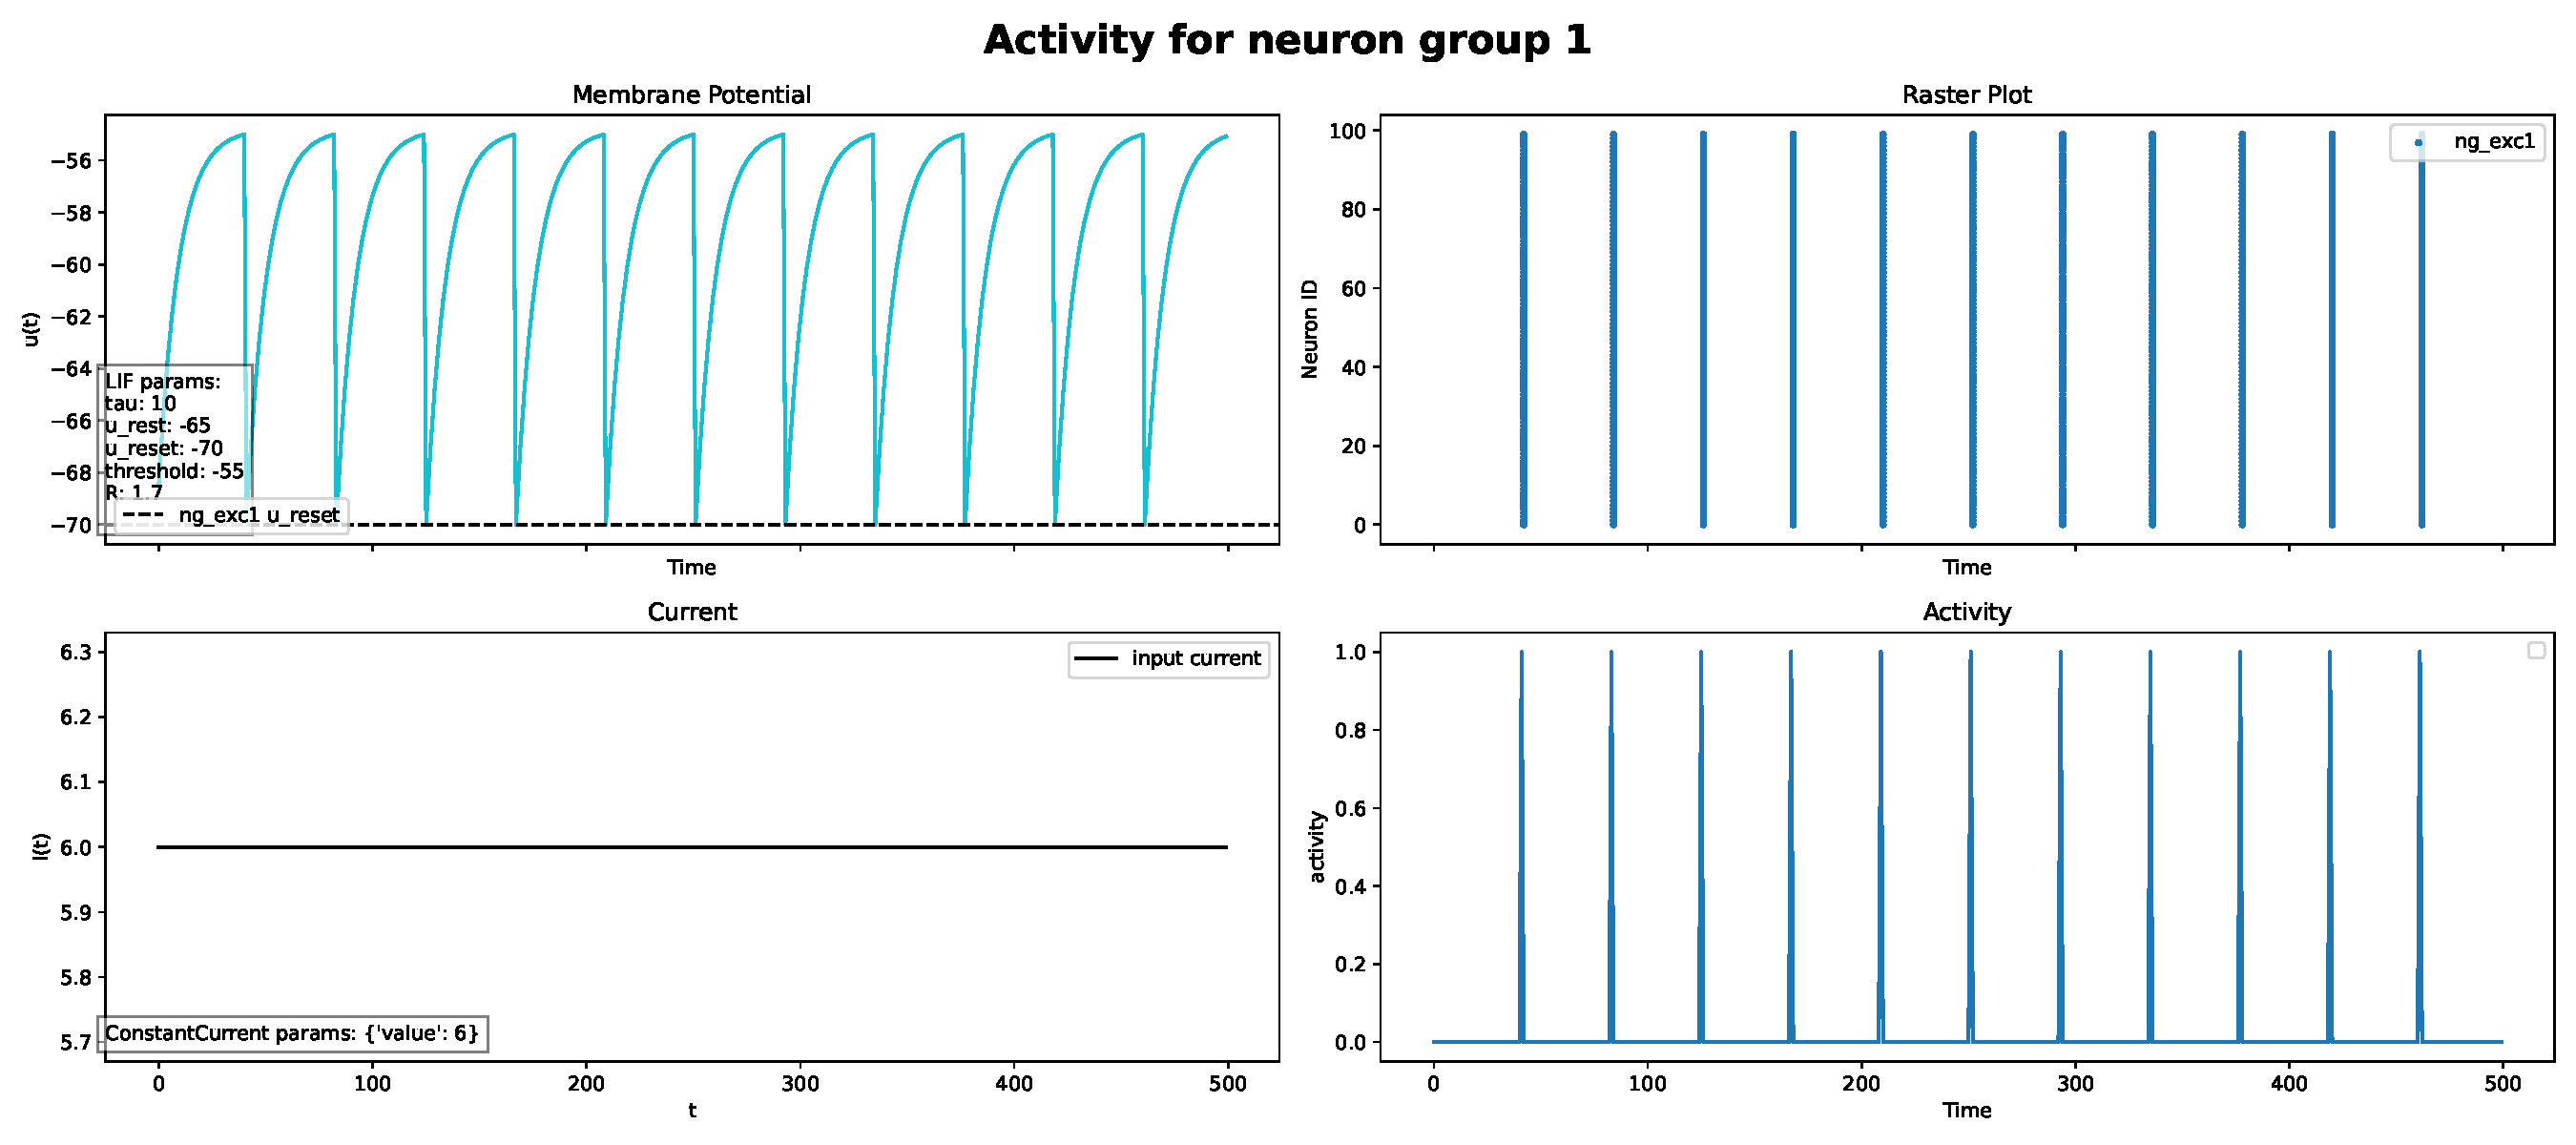
\includegraphics[width=0.9\textwidth]{plots/part1-Simple-ng-without-synapse.pdf} 
            \caption{جمعیت نورونی بدون سیناپس}
            \label{fig:part1-simple-ng}
        \end{figure}

        حال بیاید مقادیر اولیه نورون ها مانند اختلاف پتانسیل اولیه آن ها را تغییر دهیم تا رفتار آن ها را ببینیم. برای اینکار، اختلاف پتانسیل اولیه نورون ها را در حدود بازه ۶۷ با واریانس ۲ توزیع میکنیم. همانطور که در شکل
        \ref{fig:part1-simple-ng-u-init}
        نیز مشاهده می کنیم، نورون ها در ابتدا با یک اختلاف پتانسیل متفاوت شروع به فعالیت میکنند و از آنجا که جریان ورودی به آن ها نیز یکسان است، فواصل ضربه زدن خود را حفظ میکنند و با همان فواصل به ضربه زدن ادامه می دهند. در نتیجه فعالیت کلی جمعیت، به صورت دوره ای تکرار خواهد شد.
        \begin{figure}[!ht]
            \centering
            \includegraphics[width=0.9\textwidth]{plots/part1-Simple-ng-without-synapse-u\_init.pdf} 
            \caption{جمعیت نورونی بدون سیناپس: اختلاف پتانسیل اولیه متفاوت}
            \label{fig:part1-simple-ng-u-init}
        \end{figure}

        حال اگر به همین جمعیت یک جریان نویز دار اضافه کنیم چه اتفاقی می افتد؟ برای اینکار یک رفتار
        (\lr{Behavior})
        به نام 
        \texttt{NoiseCurrent}
        تعریف میکنیم که وظیفه آن اضافه کردن نویز به جریان نورون باشد. مقدار این نویز را یک جریان رندوم با میانگین ۰ و واریانس ۰.۱ قرار می دهیم. همانطور که در شکل 
        \ref{fig:part1-simple-ng-u-init-noise-curr}
        مشاهده میکنیم، به دلیل اضافه شدن نویز، الگوی فعالت نورون ها در بازه هایی که ضربه میزنند رفته رفته تغییر کرده و الگوی خود را از دست می دهند. هر چند اگر میزان این نویز خیلی زیاد باشد، می تواند برآیند جریان ورودی را زیاد کرده، به نحوی که رفتار نورون ها پس از مدتی مشابه شود.
        (شکل \ref{fig:part1-simple-ng-u-init-high-noise-curr})
        \begin{figure}[!ht]
            \centering
            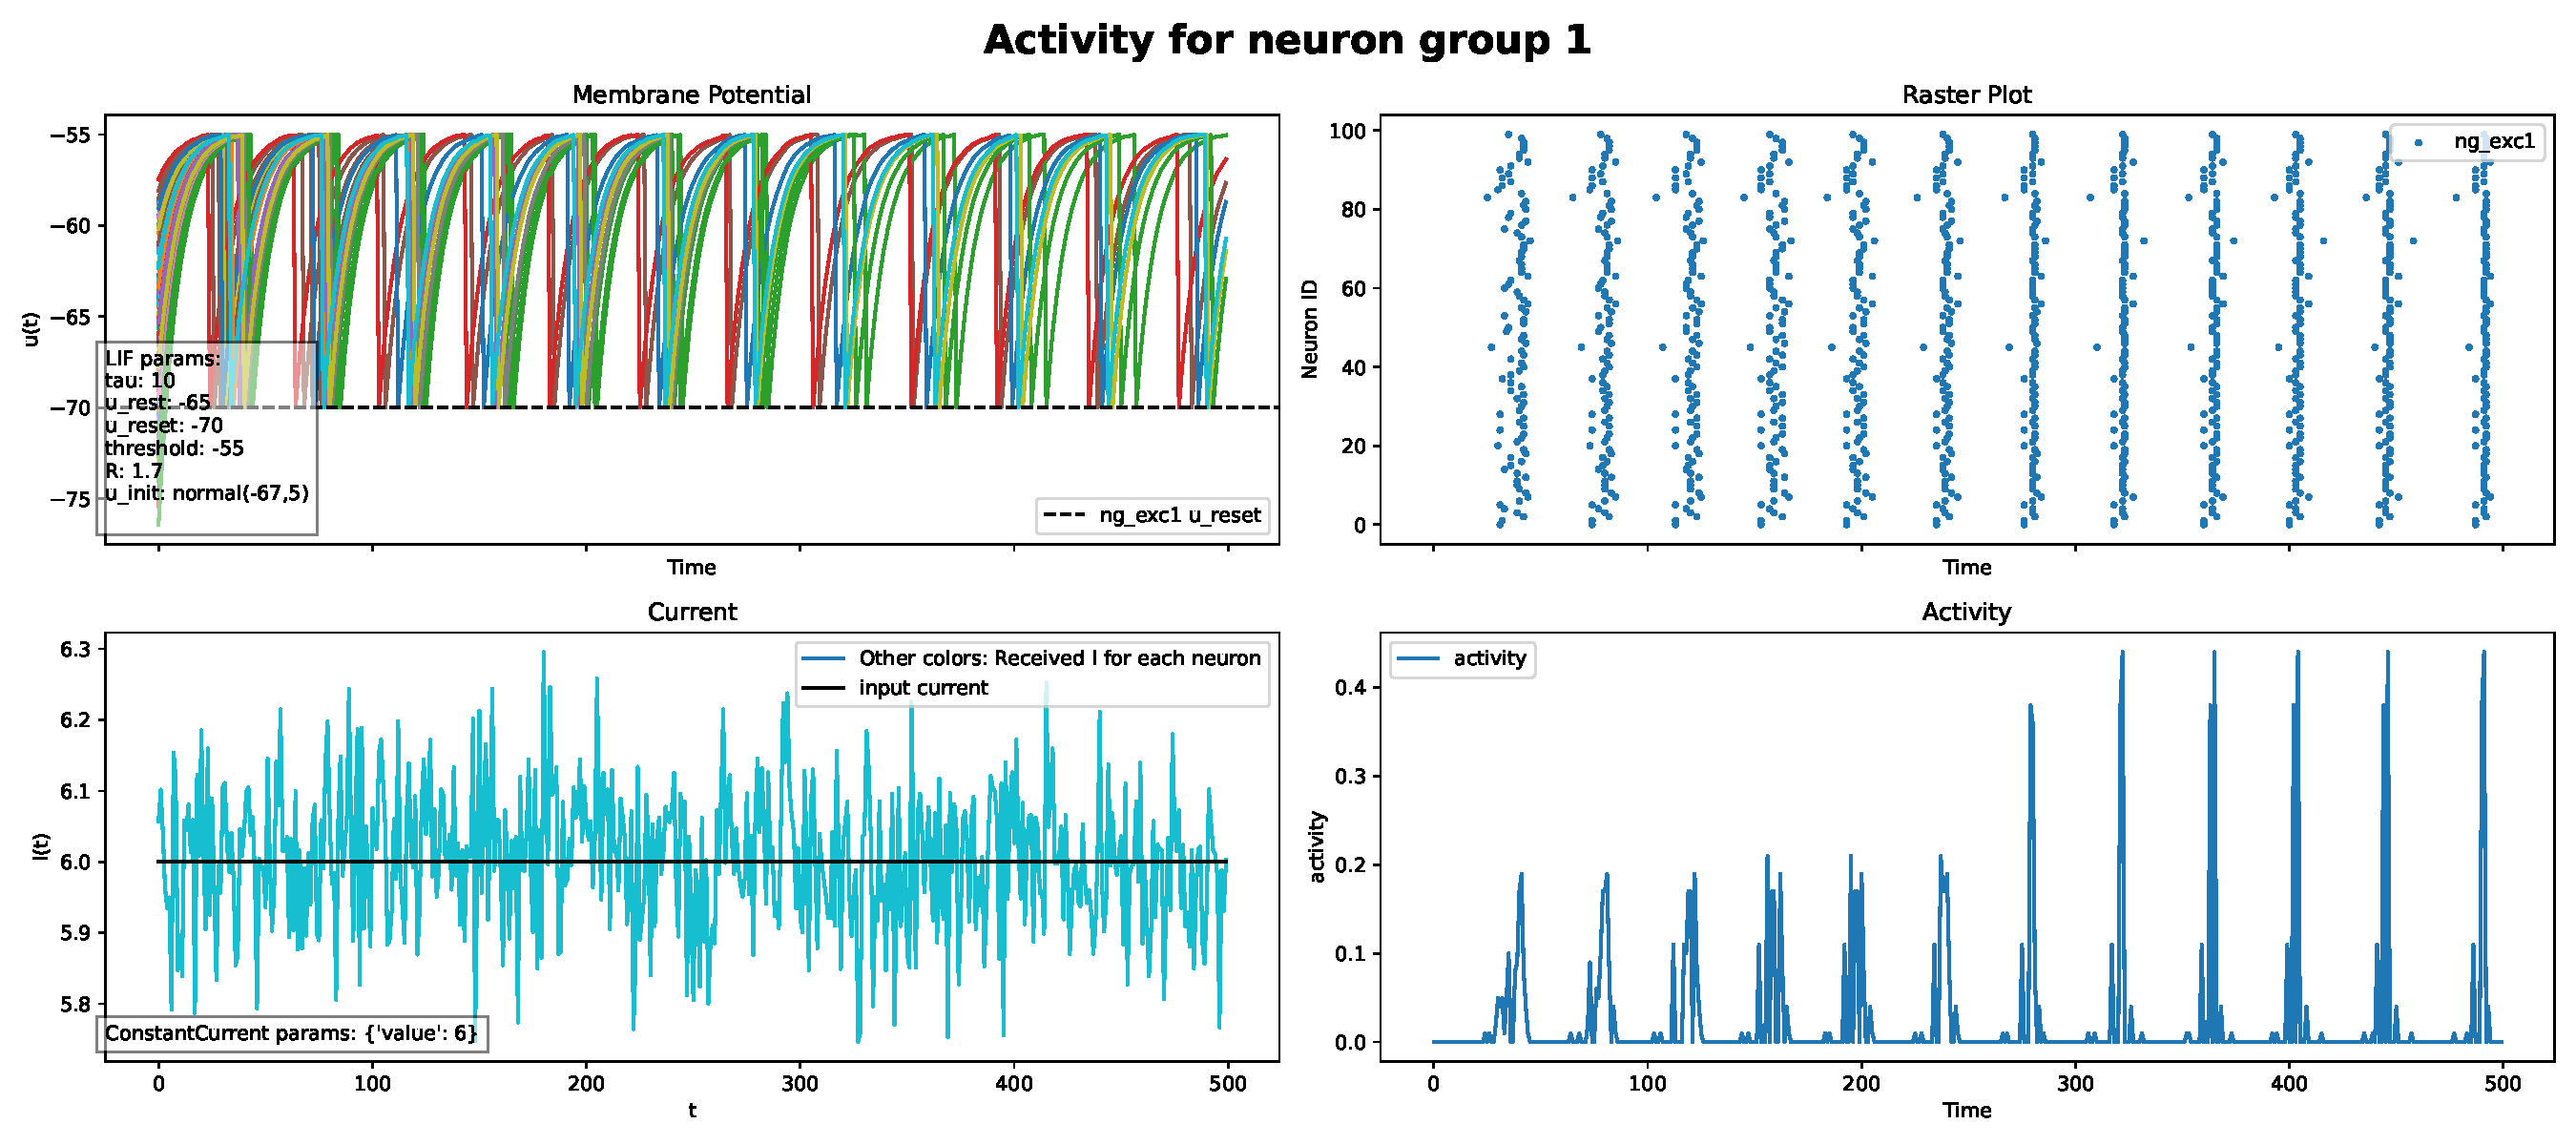
\includegraphics[width=0.9\textwidth]{plots/part1-Simple-ng-without-synapse-noise-curr.pdf} 
            \caption{جمعیت نورونی بدون سیناپس: اختلاف پتانسیل اولیه متفاوت و جریان نویزی}
            \label{fig:part1-simple-ng-u-init-noise-curr}
        \end{figure}
        \begin{figure}[!ht]
            \centering
            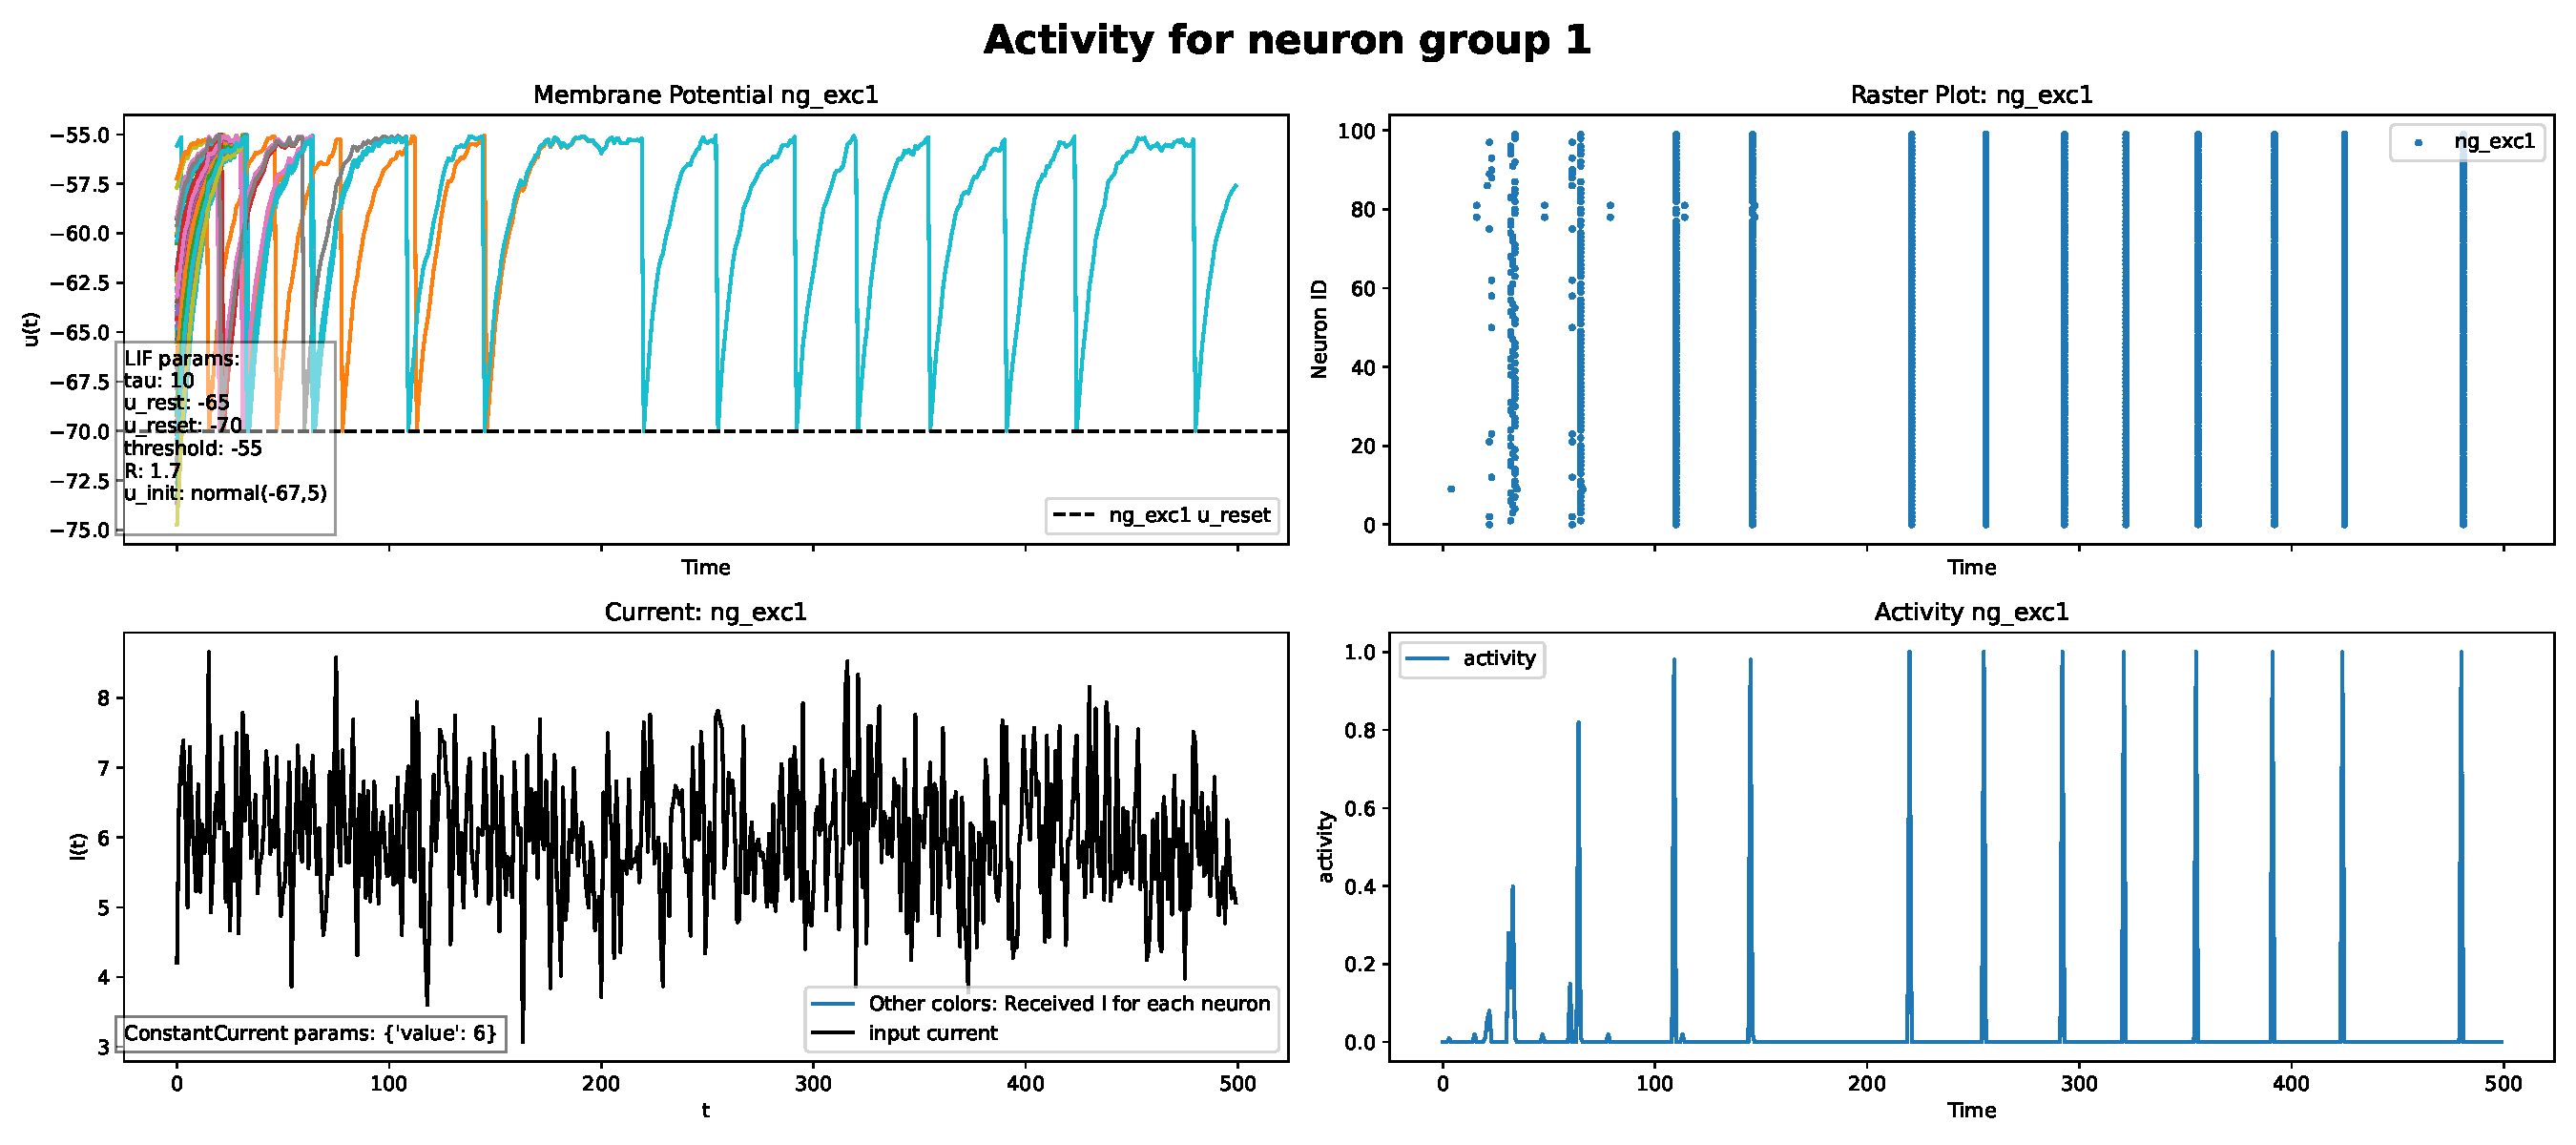
\includegraphics[width=0.9\textwidth]{plots/part1-Simple-ng-without-synapse-high-noise-curr.pdf} 
            \caption{جمعیت نورونی بدون سیناپس: اختلاف پتانسیل اولیه متفاوت و جریان نویزی زیاد}
            \label{fig:part1-simple-ng-u-init-high-noise-curr}
        \end{figure}

        حال فعالیت جمعیت نورونی را با جریان متفاوت برای هر نورون آزمایش میکنیم تا رفتار آن ها را بر این اساس نیز مشاهده کنیم. برای اینکار، جریان ورودی به جمعیت نورونی را با واریانس 
        $0.2$
        اضافه میکنیم. همانطور که در شکل 
        \ref{fig:part1-simple-ng-variance-curr}
        مشاهده میکنیم، تغییر دادن جریان ورودی به ازای هر نورون، زمان ضربه زدن هر نورون را از دیگری نسبت به حالت های قبل بیشتر متفاوت می کند و در نتیجه، پراکندگی زمان فعالیت نورون ها بیشتر می شود. همچنین اضافه کردن واریانس بیشتر میتواند پراکندگی را آنقدر افزایش دهد تا تشخیص یک الگو برای زمان ضربه زدن نورون ها بسیار سخت تر شود
        (شکل \ref{fig:part1-simple-ng-high-variance-curr})
        \begin{figure}[!ht]
            \centering
            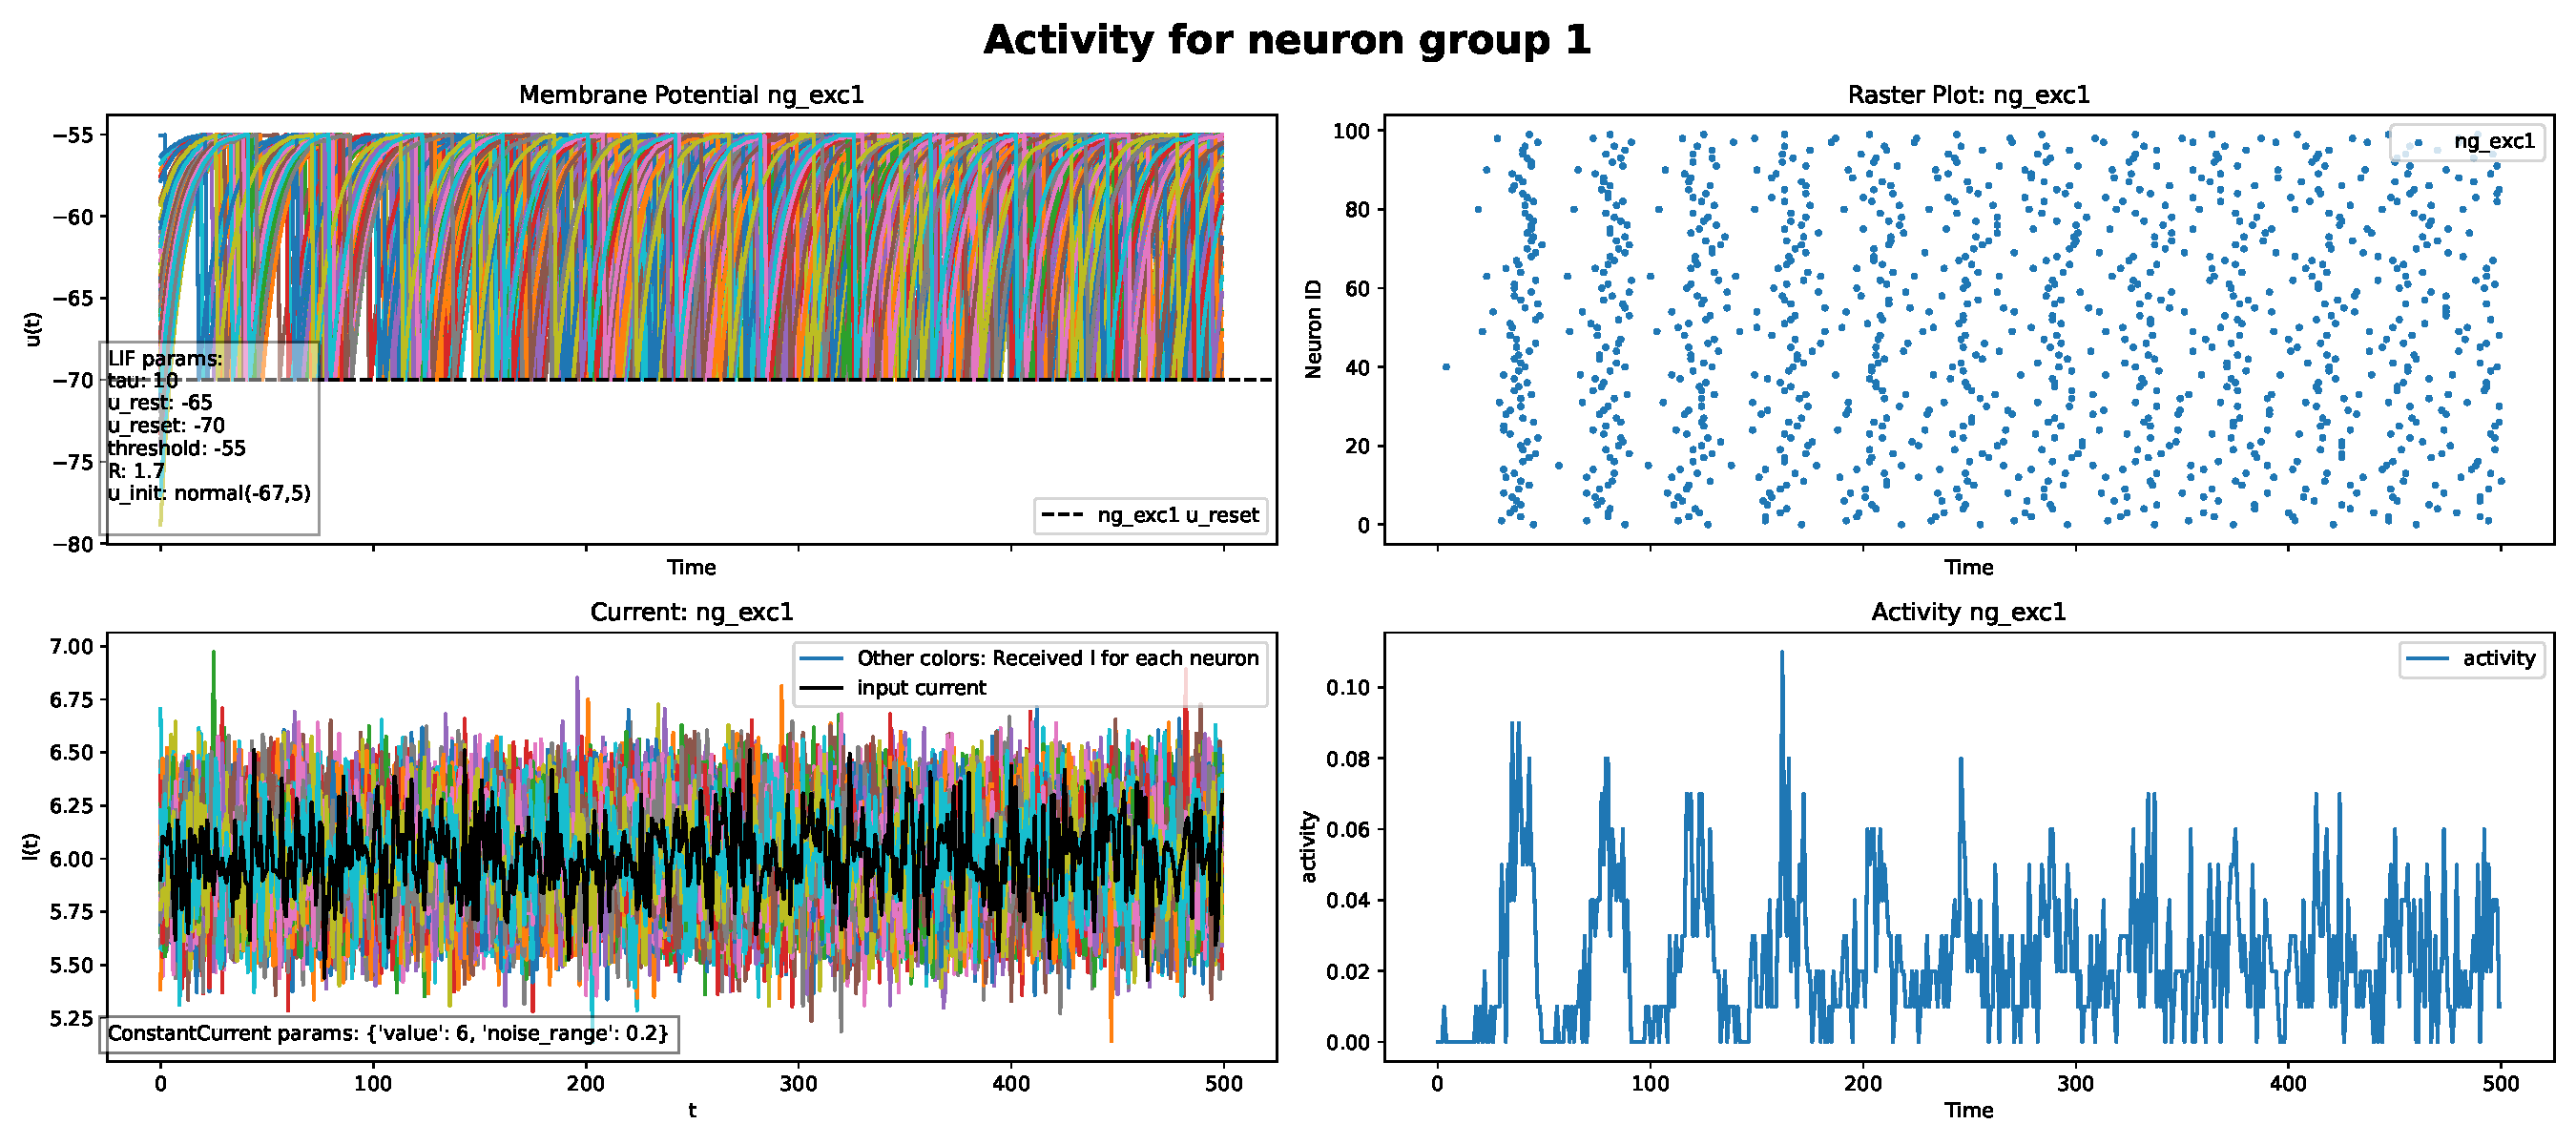
\includegraphics[width=0.9\textwidth]{plots/part1-Simple-ng-without-synapse-variance-curr.pdf} 
            \caption{جمعیت نورونی بدون سیناپس: جریان ورودی متفاوت}
            \label{fig:part1-simple-ng-variance-curr}
        \end{figure}
        \begin{figure}[!ht]
            \centering
            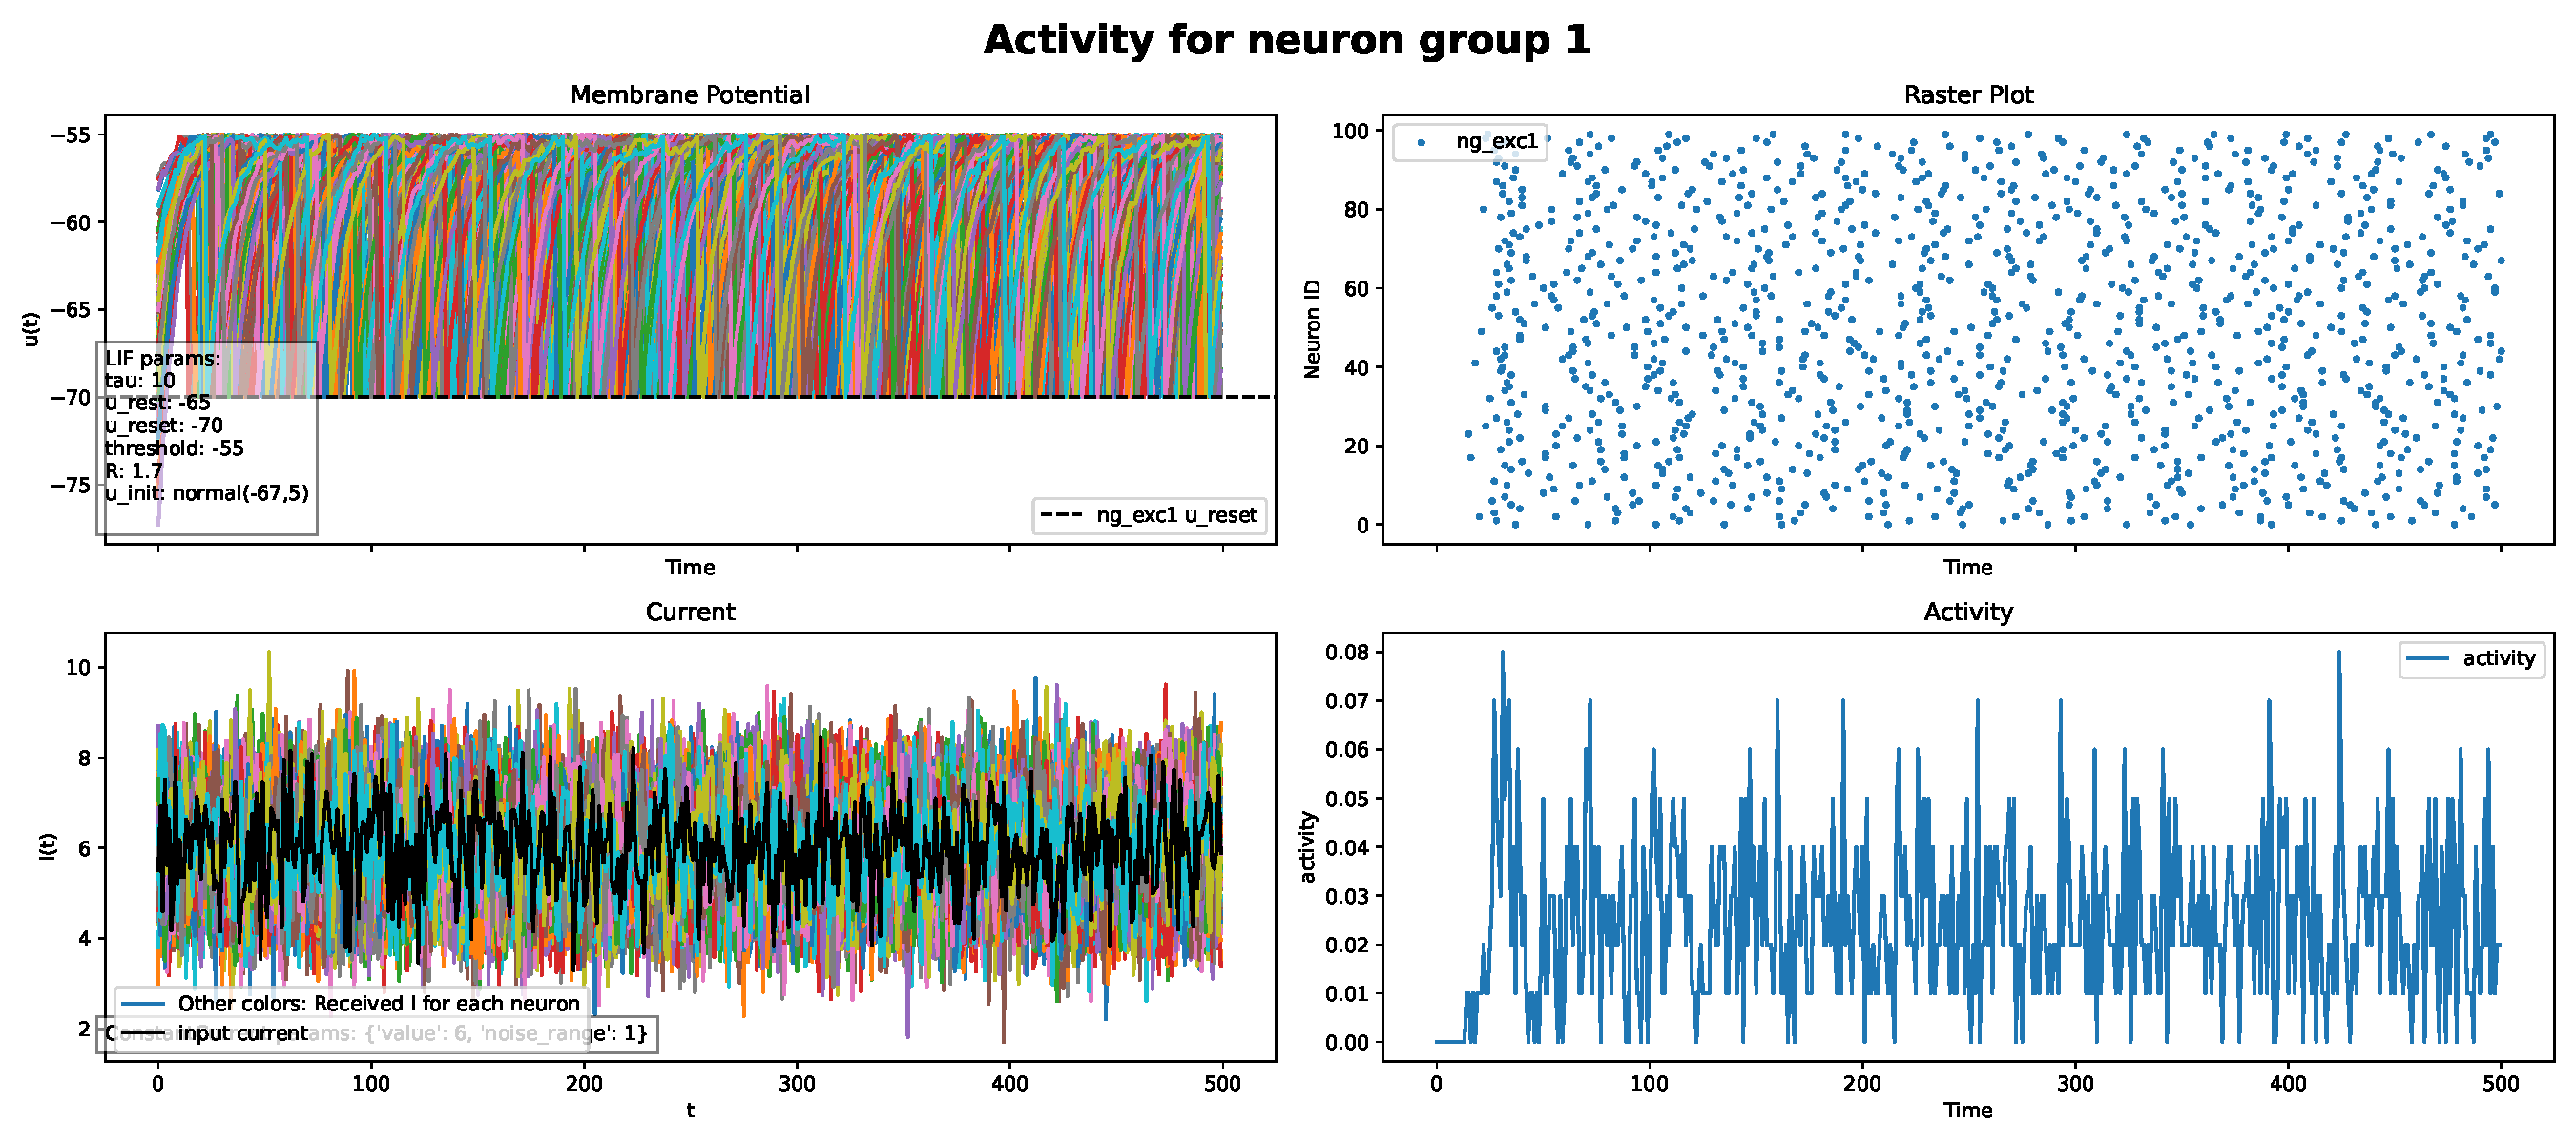
\includegraphics[width=0.9\textwidth]{plots/part1-Simple-ng-without-synapse-high-variance-curr.pdf} 
            \caption{جمعیت نورونی بدون سیناپس: جریان ورودی با تفاوت زیاد}
            \label{fig:part1-simple-ng-high-variance-curr}
        \end{figure}

        \subsubsection*{جمعیت نورونی به همراه سیناپس}
        حال که تاثیر انواع متفاوت جریان را بر یک جمعیت نورونی بررسی کردیم، به سراغ اضافه کردن سیناپس به آن میرویم. برای سادگی، سیناپس را با الگوی ارتباط کامل
        \footnote{\lr{full connectivity}}
        بررسی میکنیم و بررسی الگو های دیگر را به بخش دوم پروژه واگذار میکنیم. در ابتدا نیز وزن های سیناپسی را کامل یکسان با
        $j_0=5$ و $\sigma=0$
        در نظر میگیریم و سپس به آن واریانس اضافه میکنیم. همانطور که در شکل
        \ref{fig:part1-simple-ng-with-synapse}
        ملاحظه میکنیم، در یک جمعیت نورونی به همراه سیناپس داخلی، که نورون ها نیز در زمان اولیه اختلاف پتانسیل یکسانی دارند، رفتار جمعیت همانند هنگامی است که سیناپس وجود نداشته باشد. این به این دلیل است که در این حالت، قبل از اولین ضربه سیناپس تاثیری ندارد و رفتار نورون  همانند جمعیت بدون سیناپس با جریان ورودی ثابت است. از این رو اختلاف پتانسیل نورون ها به طور همزمان افزایش می یابد تا هنگامی که به  آستانه رسیده و نورون ها همزمان ضربه می زنند. در این لحظه، بلافاصله جریان سیناپسی نیز به جریان دریافتی نورون اضافه می شود و از آنجا که سیناپس ارتباط کامل است، زمان ضربه زدن نورون ها تغییری پیدا نمی کند.
        \begin{figure}[!ht]
            \centering
            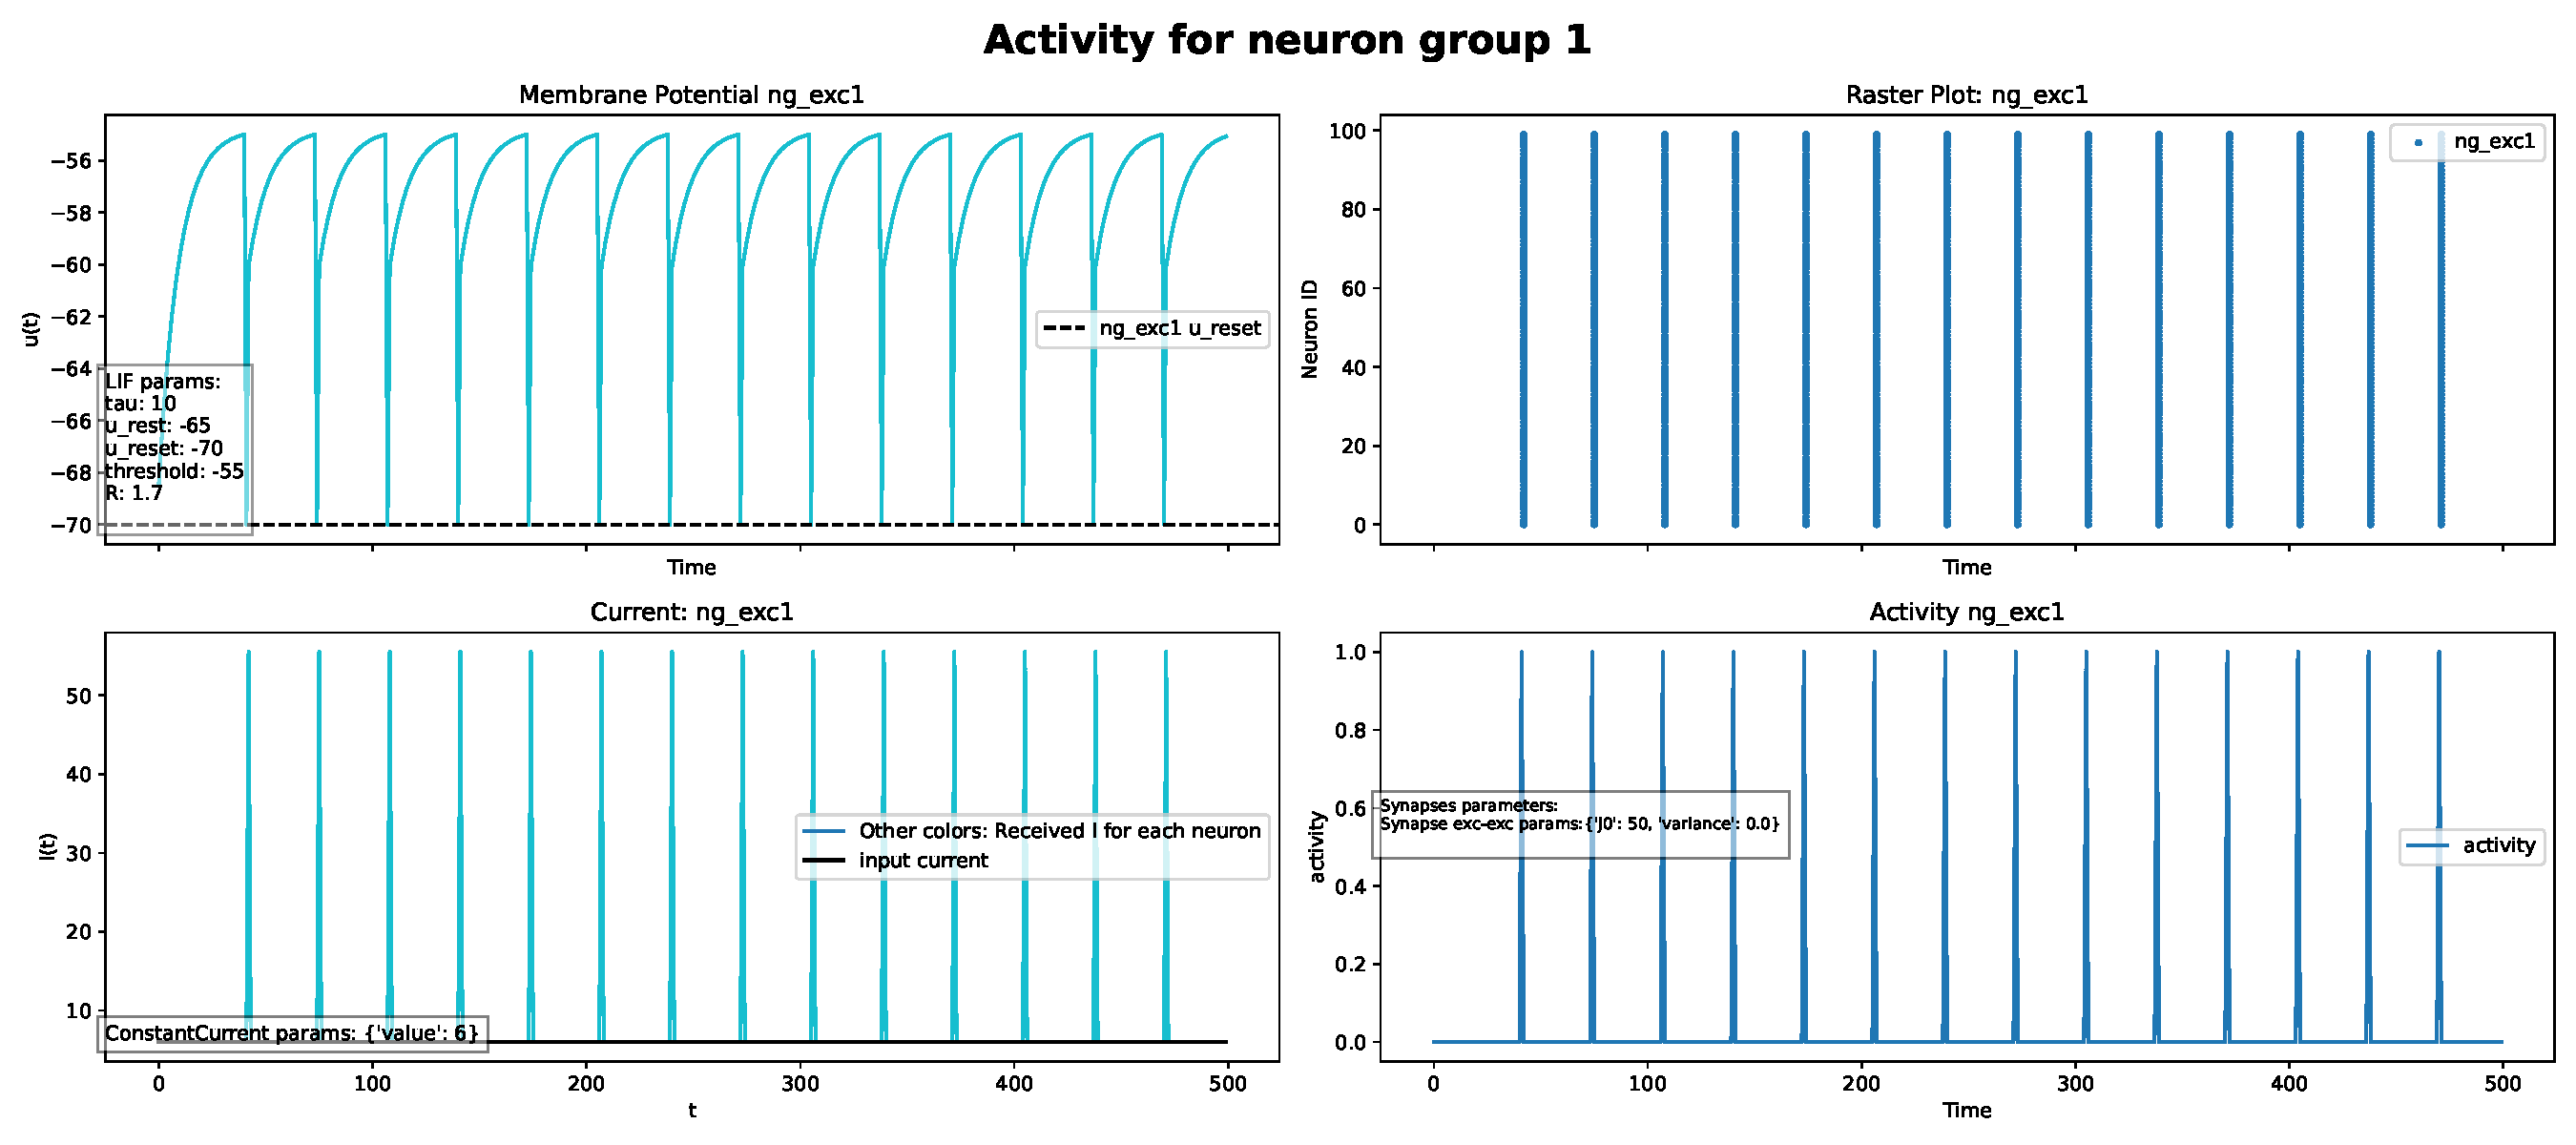
\includegraphics[width=0.9\textwidth]{plots/part1-Simple-ng-with-synapse.pdf} 
            \caption{جمعیت نورونی با سیناپس: جریان ثابت}
            \label{fig:part1-simple-ng-with-synapse}
        \end{figure}

        حال اگر اختلاف پتانسیل اولیه نورون ها را متفاوت مقدار دهی کنیم، مطابق شکل
        \ref{fig:part1-simple-ng-with-synapse-u-init}
        میبینیم که زمان ضربه زدن نورون ها متفاوت می شود.هر چند پس از مدتی، به دلیل اضافه شدن جریان سیناپسی به جریان ورودی نورون و درنتیجه افزایش یافتن جریان دریافتی نورون، این اختلاف زمانی ضربه ها نیز کمتر می شود. افزایش مقدار 
        $j_0$ 
        به ۱۰ نیز زمان این همگرایی را سریع تر می کند.
        (شکل \ref{fig:part1-simple-ng-with-synapse-u-init-high-j})
        \begin{figure}[!ht]
            \centering
            \includegraphics[width=0.9\textwidth]{plots/part1-Simple-ng-with-synapse-u\_init.pdf} 
            \caption{جمعیت نورونی با سیناپس: اختلاف پتانسیل اولیه متفاوت}
            \label{fig:part1-simple-ng-with-synapse-u-init}
        \end{figure}
        \begin{figure}[!ht]
            \centering
            \includegraphics[width=0.9\textwidth]{plots/part1-Simple-ng-with-synapse-u\_init-high\_j.pdf} 
            \caption{جمعیت نورونی با سیناپس: اختلاف پتانسیل اولیه متفاوت و وزن های بیشتر}
            \label{fig:part1-simple-ng-with-synapse-u-init-high-j}
        \end{figure}

        حال واریانس وزن های سیناپسی را از ۰ بیشتر میکنیم، تا تاثیر این پارامتر را بر روی رفتار جمعیت ملاحظه کنیم. انتظار داریم که افزودن پراکندگی به وزن ها باعث پراکندگی زمان ضربه زدن نورون ها نیز بشود. شکل 

        این موضوع را تایید میکند و ملاظحه می شود که فعالیت نورون ها مانند شکل قبل همگرا نشده و بالا و پایین می شود
        (در نهایت بین مقادیر ۰.۶ و ۰.۸ نوسان می کند.)

        بعد از بررسی پارامتر های سیناپس، نوبت به بررسی تاثیر جریان بر روی سیناپس می رسد. مطابق زیربخش قبل، در ابتدا رفتار جمعیت را با جریان نویزی یکسان برای همه نورون ها بررسی میکنیم. همانطور که در شکل
        \ref{fig:part1-simple-ng-with-synapse-noise-curr}
        مشاهده می شود، در ابتدا، زمان ضربه زدن نورون ها با یکدیگر متفاوت است و پس از مدتی این تفاوت کاهش یافته و همگرا می شود به طور که در نمودار فعالیت مشاهده می کنیم که ابتدا فعالیت نورونی حدود ۰ بوده و در نهایت به ۱ می رسد.
        \begin{figure}[!ht]
            \centering
            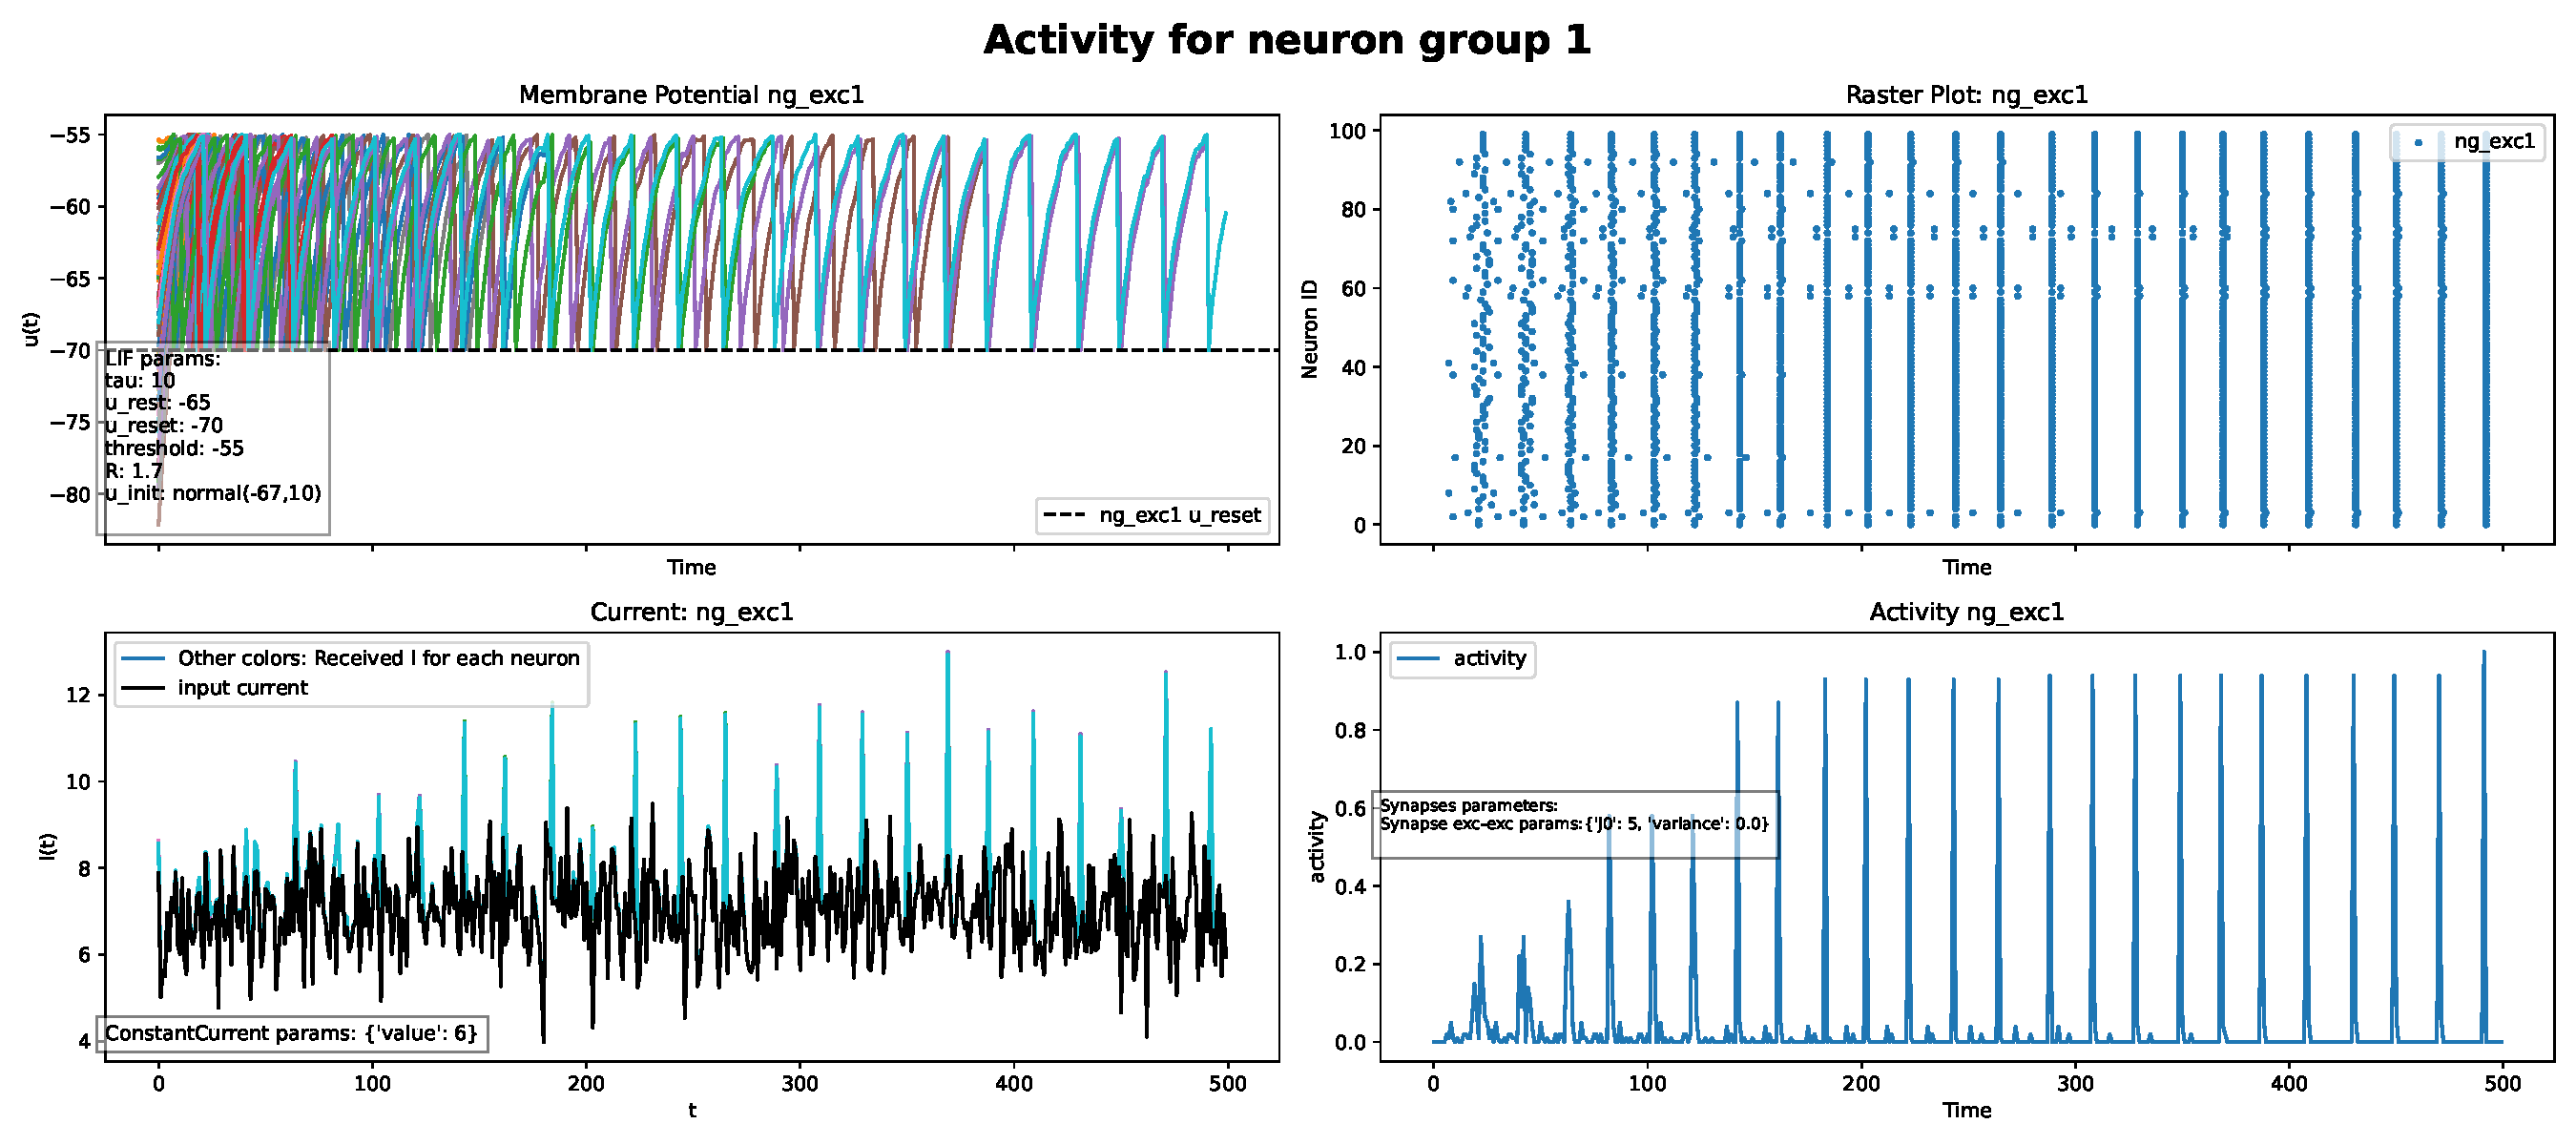
\includegraphics[width=0.9\textwidth]{plots/part1-Simple-ng-with-synapse-noise-curr.pdf} 
            \caption{جمعیت نورونی با سیناپس: اختلاف پتانسیل اولیه متفاوت و جریان نویز دار}
            \label{fig:part1-simple-ng-with-synapse-noise-curr}
        \end{figure}

        اکنون نوبت به آزمایش رفتار جمعیت نسبت به جریان متفاوت می رسد. در این آزمایش، رفتار جمعیت را با جریان نویزی برای نورون های مختلف با دامنه نوسان 0.6 بررسی میکنیم. همانطور که در شکل
        \ref{fig:part1-simple-ng-with-synapse-diff-curr}
        مشاهده می شود، داشتن جریان های متفاوت سبب می شود که زمان ضربه زدن نورون ها پارکندگی بیشتر نسبت به قبل داشته باشد ولی برخلاف جمعیت بدون سیناپس که این پراکندگی کاهش نمی یافت، در جمعیت دارای سیناپس مشاهده میکنیم که پس از مدتی، پراکندگی زمان ضربه زدن نورون ها کاهش یافته و در نتیجه فعالیت جمعیت بیشتر میشود.
        \begin{figure}[!ht]
            \centering
            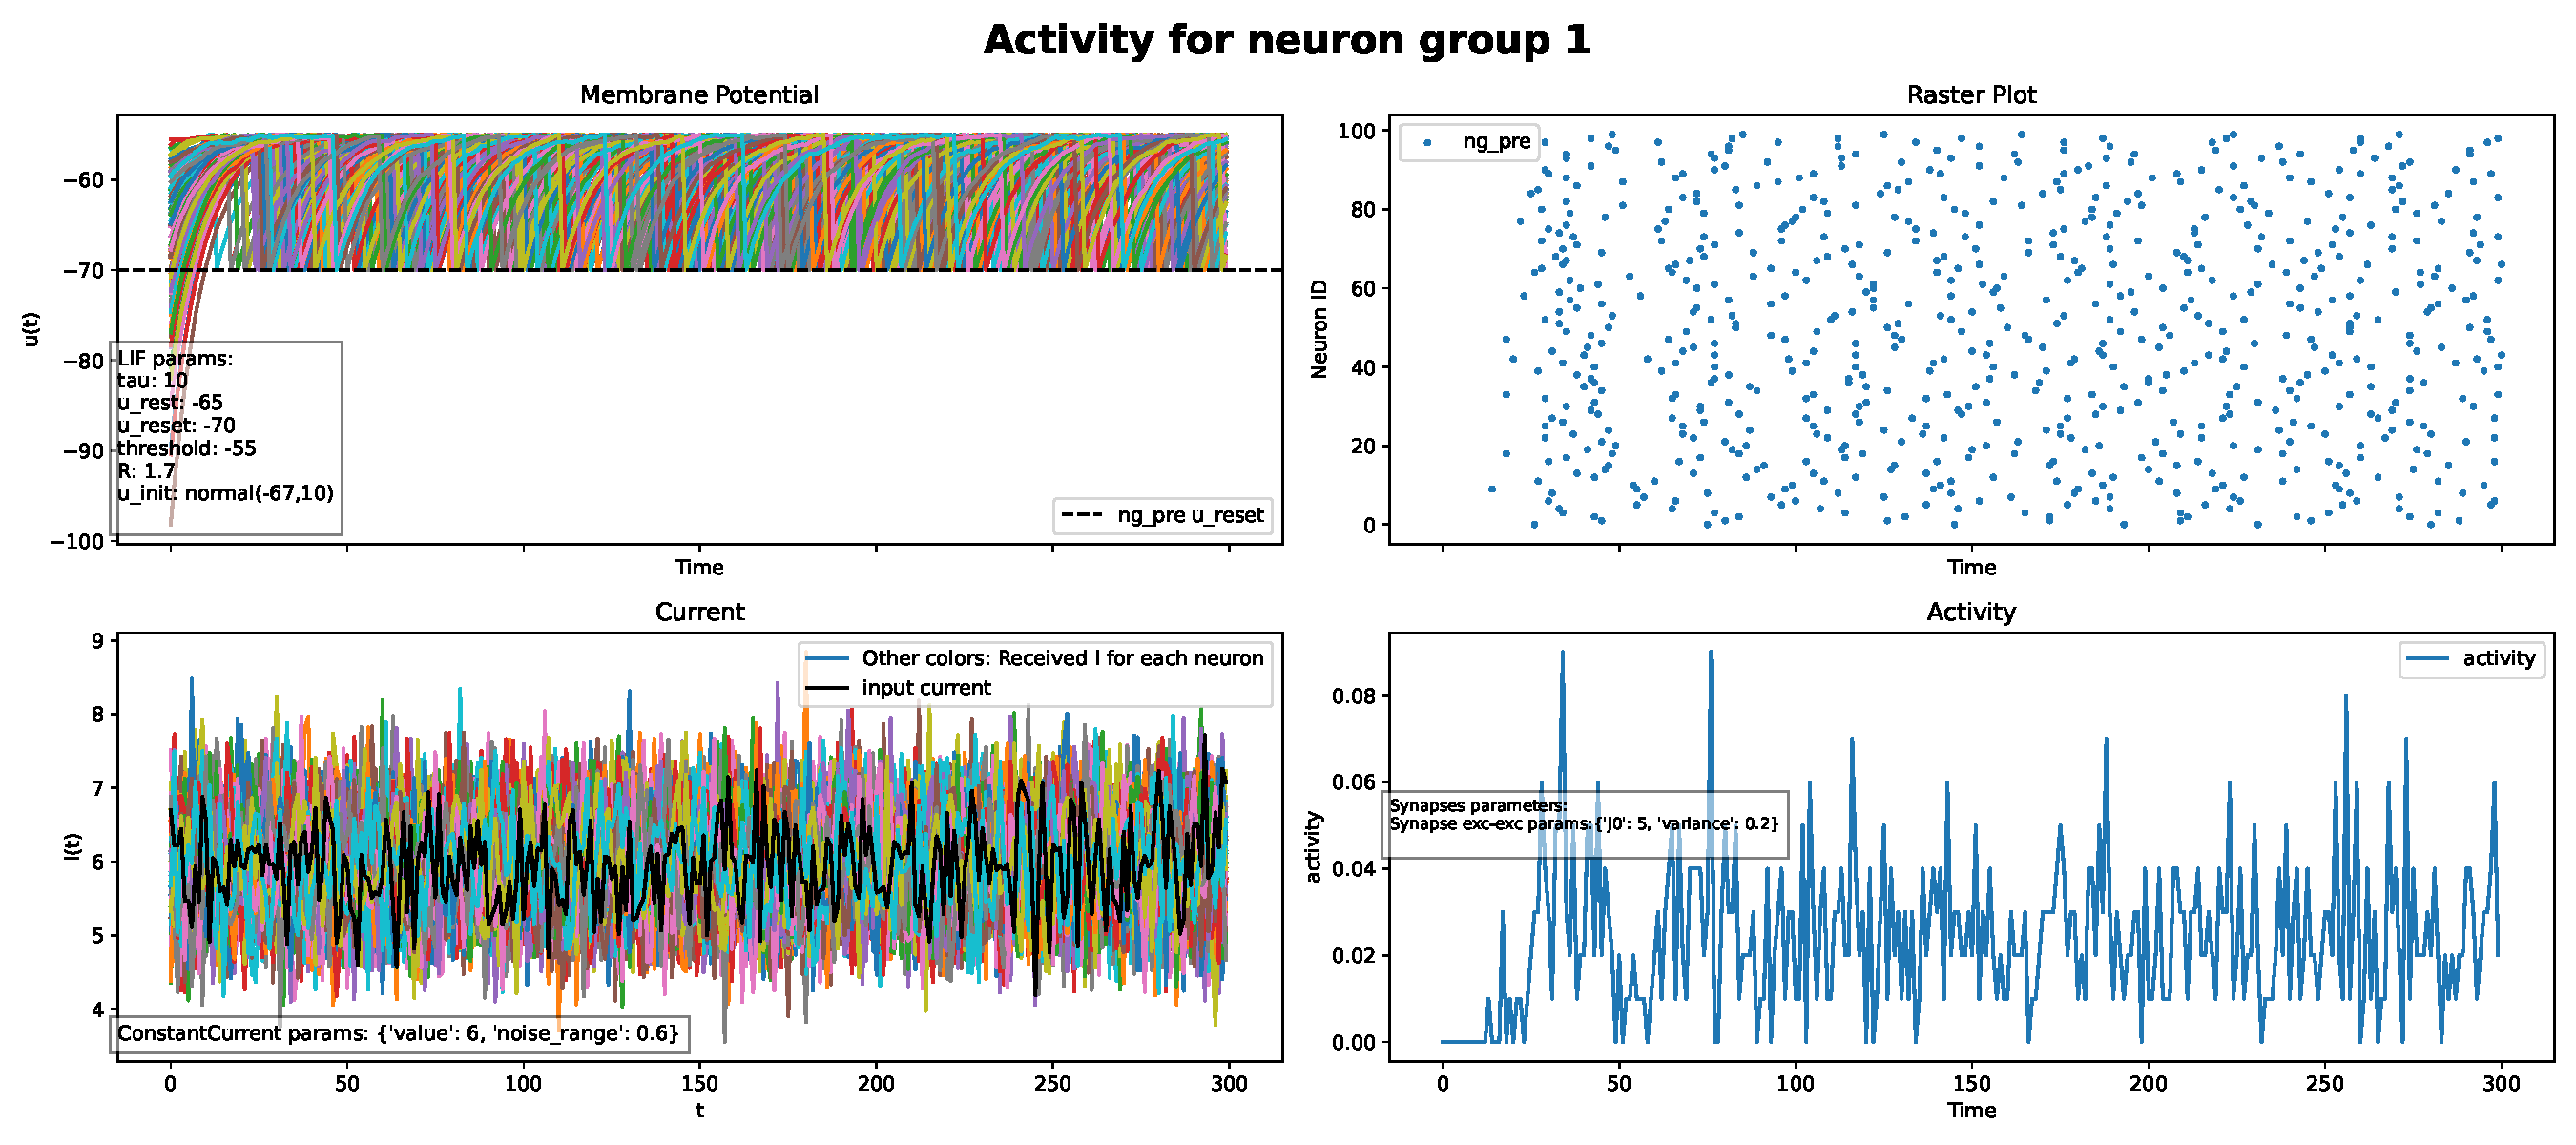
\includegraphics[width=0.9\textwidth]{plots/part1-Simple-ng-with-synapse-diff-curr.pdf} 
            \caption{جمعیت نورونی با سیناپس: اختلاف پتانسیل اولیه متفاوت و جریان نویزی غیریکسان}
            \label{fig:part1-simple-ng-with-synapse-diff-curr}
        \end{figure}

    \subsection{بررسی رفتار دو جمعیت نورونی}
        پس از بررسی رفتار یک جمعیت نورونی در حضور سیناپس، اکنون به سراغ بررسی رفتار دو جمعیت نورونی که از یکی به دیگری سیناپس وجود دارد می رویم. در این بخش تنها حالتی را در نظر میگیریم که یک جمعیت، نورون های پیش سیناپسی را تشکیل داده و جمعیت دیگر نورون های پس سیناپسی. بررسی حالت هایی با سیناپس های بیشتر را به بخش های بعدی واگذار میکنیم.

        برای اینکار، ابتدا دو جمعیت نورونی تحریکی کاملا مشابه تشکیل میدهیم که فقط از جمعیت اول به جمعیت دوم سیناپس داریم. همچنین جریان ورودی هر دو جمعیت را نیز یکسان و ثابت میگیریم. حال اگر شبیه سازی را انجام دهیم، در شکل
        \ref{fig:part1-two-ng-with-synapse}
        ملاحظه میکنیم که زمان ضربه زدن نورون های هر دو جمعیت کاملا یکسان است که این موضوع مربوط به کاملا یکسان بودن این دو جمعیت است. همچنین به دلیل اینکه در پیاده سازی سیناپس، طبق گفته حل تمرین مربوطه، نیازی نیست تا تاثیر سیناپس تا لحظات بعد نیز باقی بماند، عملا افزایش لحظه ای جریان ورودی به نورون های پس سیناپسی بی تاثیر می شود. اما اگر بتوان تاثیر جریان های موجود در سیناپس را حفظ نمود، ضربه های نورون پیش سیناپسی نیز روی نورون های پس سیناپسی تاثیر گذار خواهد بود
        (شکل \ref{fig:part1-two-ng-with-synapse-decay})
        \begin{figure}[!ht]
            \centering
            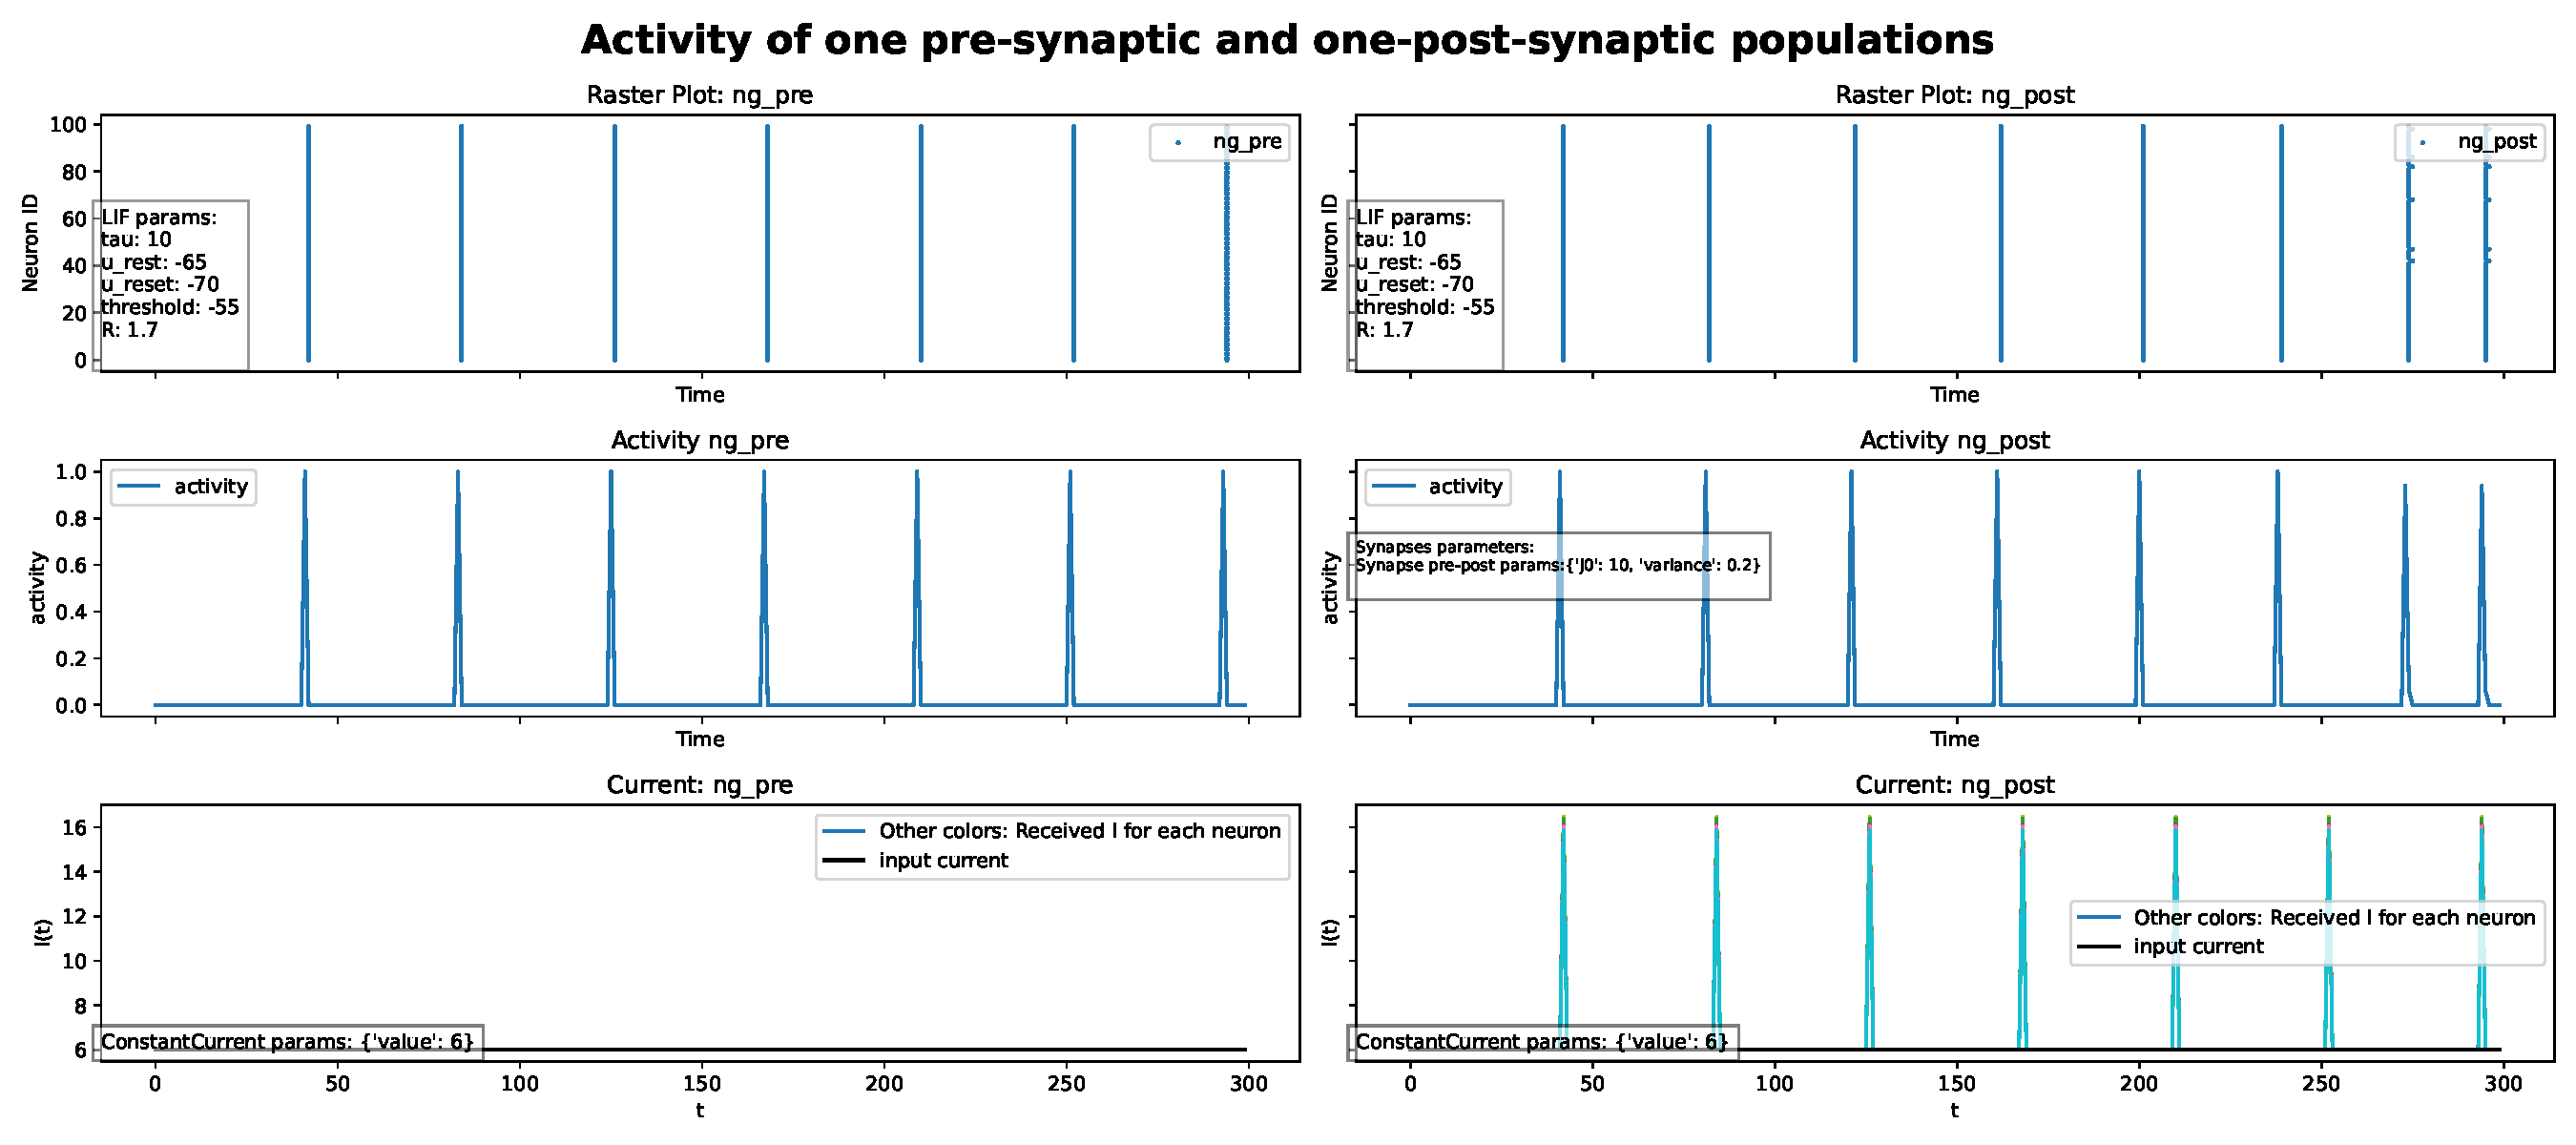
\includegraphics[width=0.9\textwidth]{plots/part1-two-ng-with-synapse.pdf} 
            \caption{جمعیت نورونی پیش سیناپسی و پس سیناپسی}
            \label{fig:part1-two-ng-with-synapse}
        \end{figure}
        \begin{figure}[!ht]
            \centering
            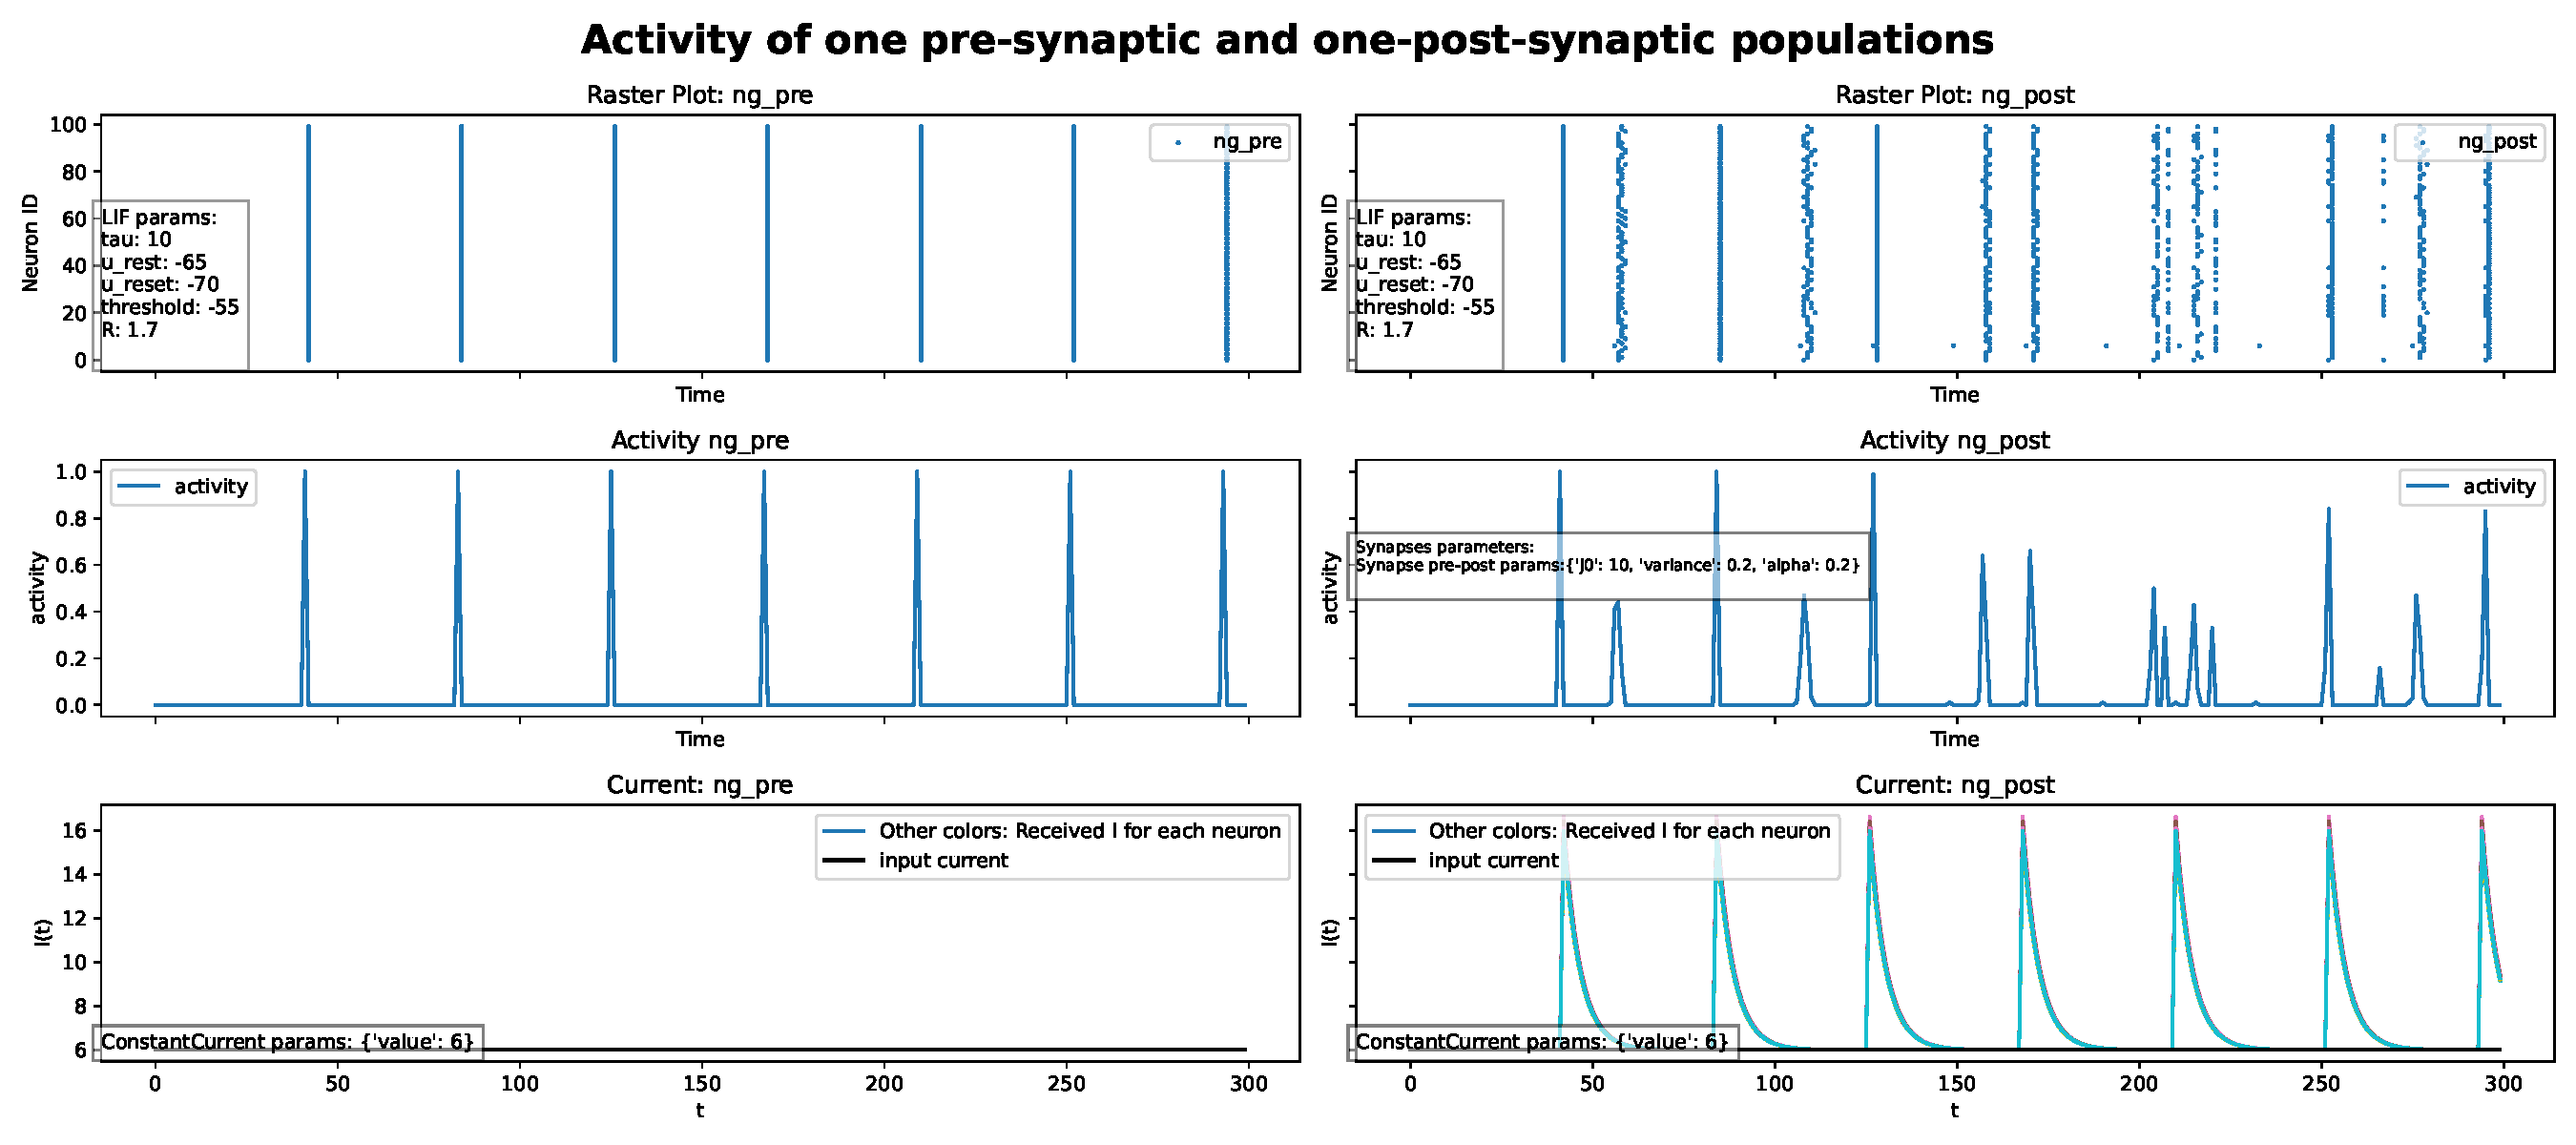
\includegraphics[width=0.9\textwidth]{plots/part1-two-ng-with-synapse-decay.pdf} 
            \caption{جمعیت نورونی پیش سیناپسی و پس سیناپسی: حفظ تاثیر جریان سیناپسی تا لحظات بعد}
            \label{fig:part1-two-ng-with-synapse-decay}
        \end{figure}
        به دلیل اینکه این نوع سیناپس هدف اصلی پروژه نمی باشد، ما بررسی های خود را بیشتر روی همان حالت گفته شده توسط دستیار آموزشی انجام می دهیم.
        
        حال اگر به نمودار 
        \ref{fig:part1-two-ng-with-synapse}
        اختلاف پتانسیل اولیه متفاوت بیفزاییم، طبق شکل 
        \ref{fig:part1-two-ng-with-synapse-u-init}
        ملاحظه میکنیم که فواصل زمانی ضربه ها در جمعیت دوم نزدیک تر بوده و فعالیت آن نسبت به جمعیت اول بیشتر است. این به این دلیل است که در جمعیت دوم، علاوه بر جریان ورودی، جریان سیناپسی که از جمعیت اول گرفته می شود نیز وجود دارد.
        \begin{figure}[!ht]
            \centering
            \includegraphics[width=0.9\textwidth]{plots/part1-two-ng-with-synapse-u\_init.pdf} 
            \caption{جمعیت نورونی پیش سیناپسی و پس سیناپسی: تاثیر اختلاف پتانسیل اولیه متفاوت}
            \label{fig:part1-two-ng-with-synapse-u-init}
        \end{figure}

        حال به جریان ورودی هر دو جمعیت، یک جریان یکسان نویز دار اضافه میکنیم. همانطور که در شکل
        \ref{fig:part1-two-ng-with-synapse-noise-curr}
        ملاحظه میکنیم، با اینکه نویز اضافه شده به هر دو نمودار از توزیع یکسان
        (میانگین=۰ و واریانس=۱)
        پیروی میکند، جریان دریافتی نهایی نورون های جمعیت پس سیناپسی، به طور میانگین بیشتر از جمعیت نورونی پیش سیناپسی است و در نتیجه فعالیت جمعیت آن نیز بیشتر است. این به این دلیل است که جریانی تحت تاثیر ضربه های جمعیت پیش سیناپسی به جریان جمعیت پس سیناپسی نیز اضافه می شود.
        \begin{figure}[!ht]
            \centering
            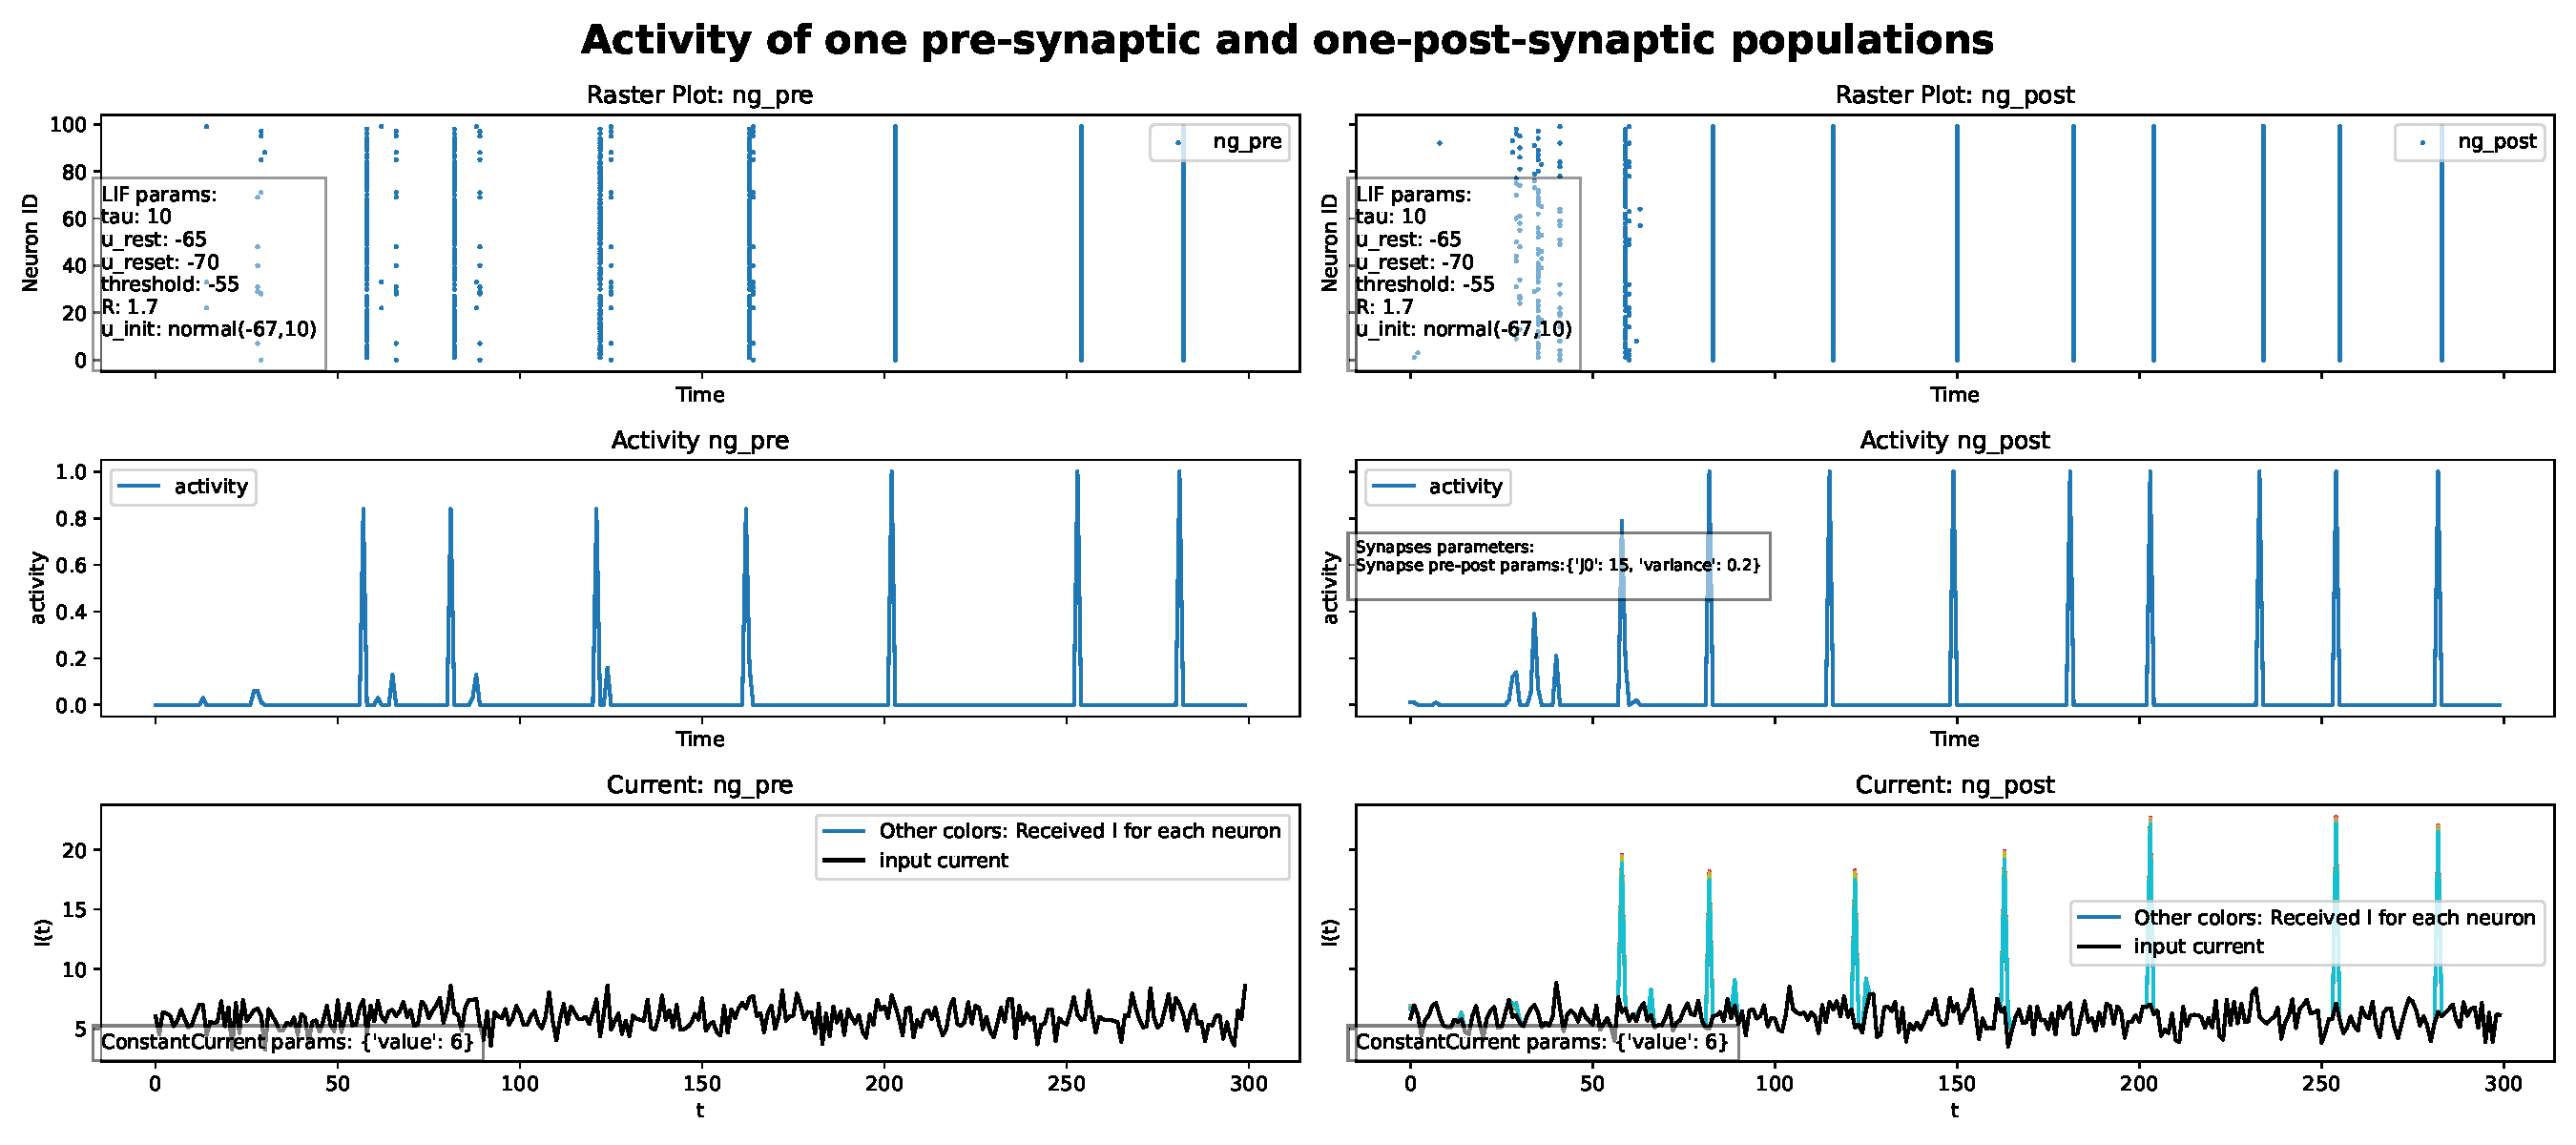
\includegraphics[width=0.9\textwidth]{plots/part1-two-ng-with-synapse-noise-curr.pdf} 
            \caption{جمعیت نورونی پیش سیناپسی و پس سیناپسی: تاثیر جریان نویزی}
            \label{fig:part1-two-ng-with-synapse-noise-curr}
        \end{figure}

        حال رفتار جمعیت را با جریان نویزی غیریکسان آزمایش میکنیم. دامنه نوسان را 
        $0.2$ 
        تنظیم میکنیم و انتظار داریم که مانند شکل های گذشته، میزان پراکندگی زمان ضربه زدن های نورون ها بیشتر شود، که از شکل 
        \ref{fig:part1-two-ng-with-synapse-diff-curr}
        نیز همین دریافت می شود.
        \begin{figure}[!ht]
            \centering
            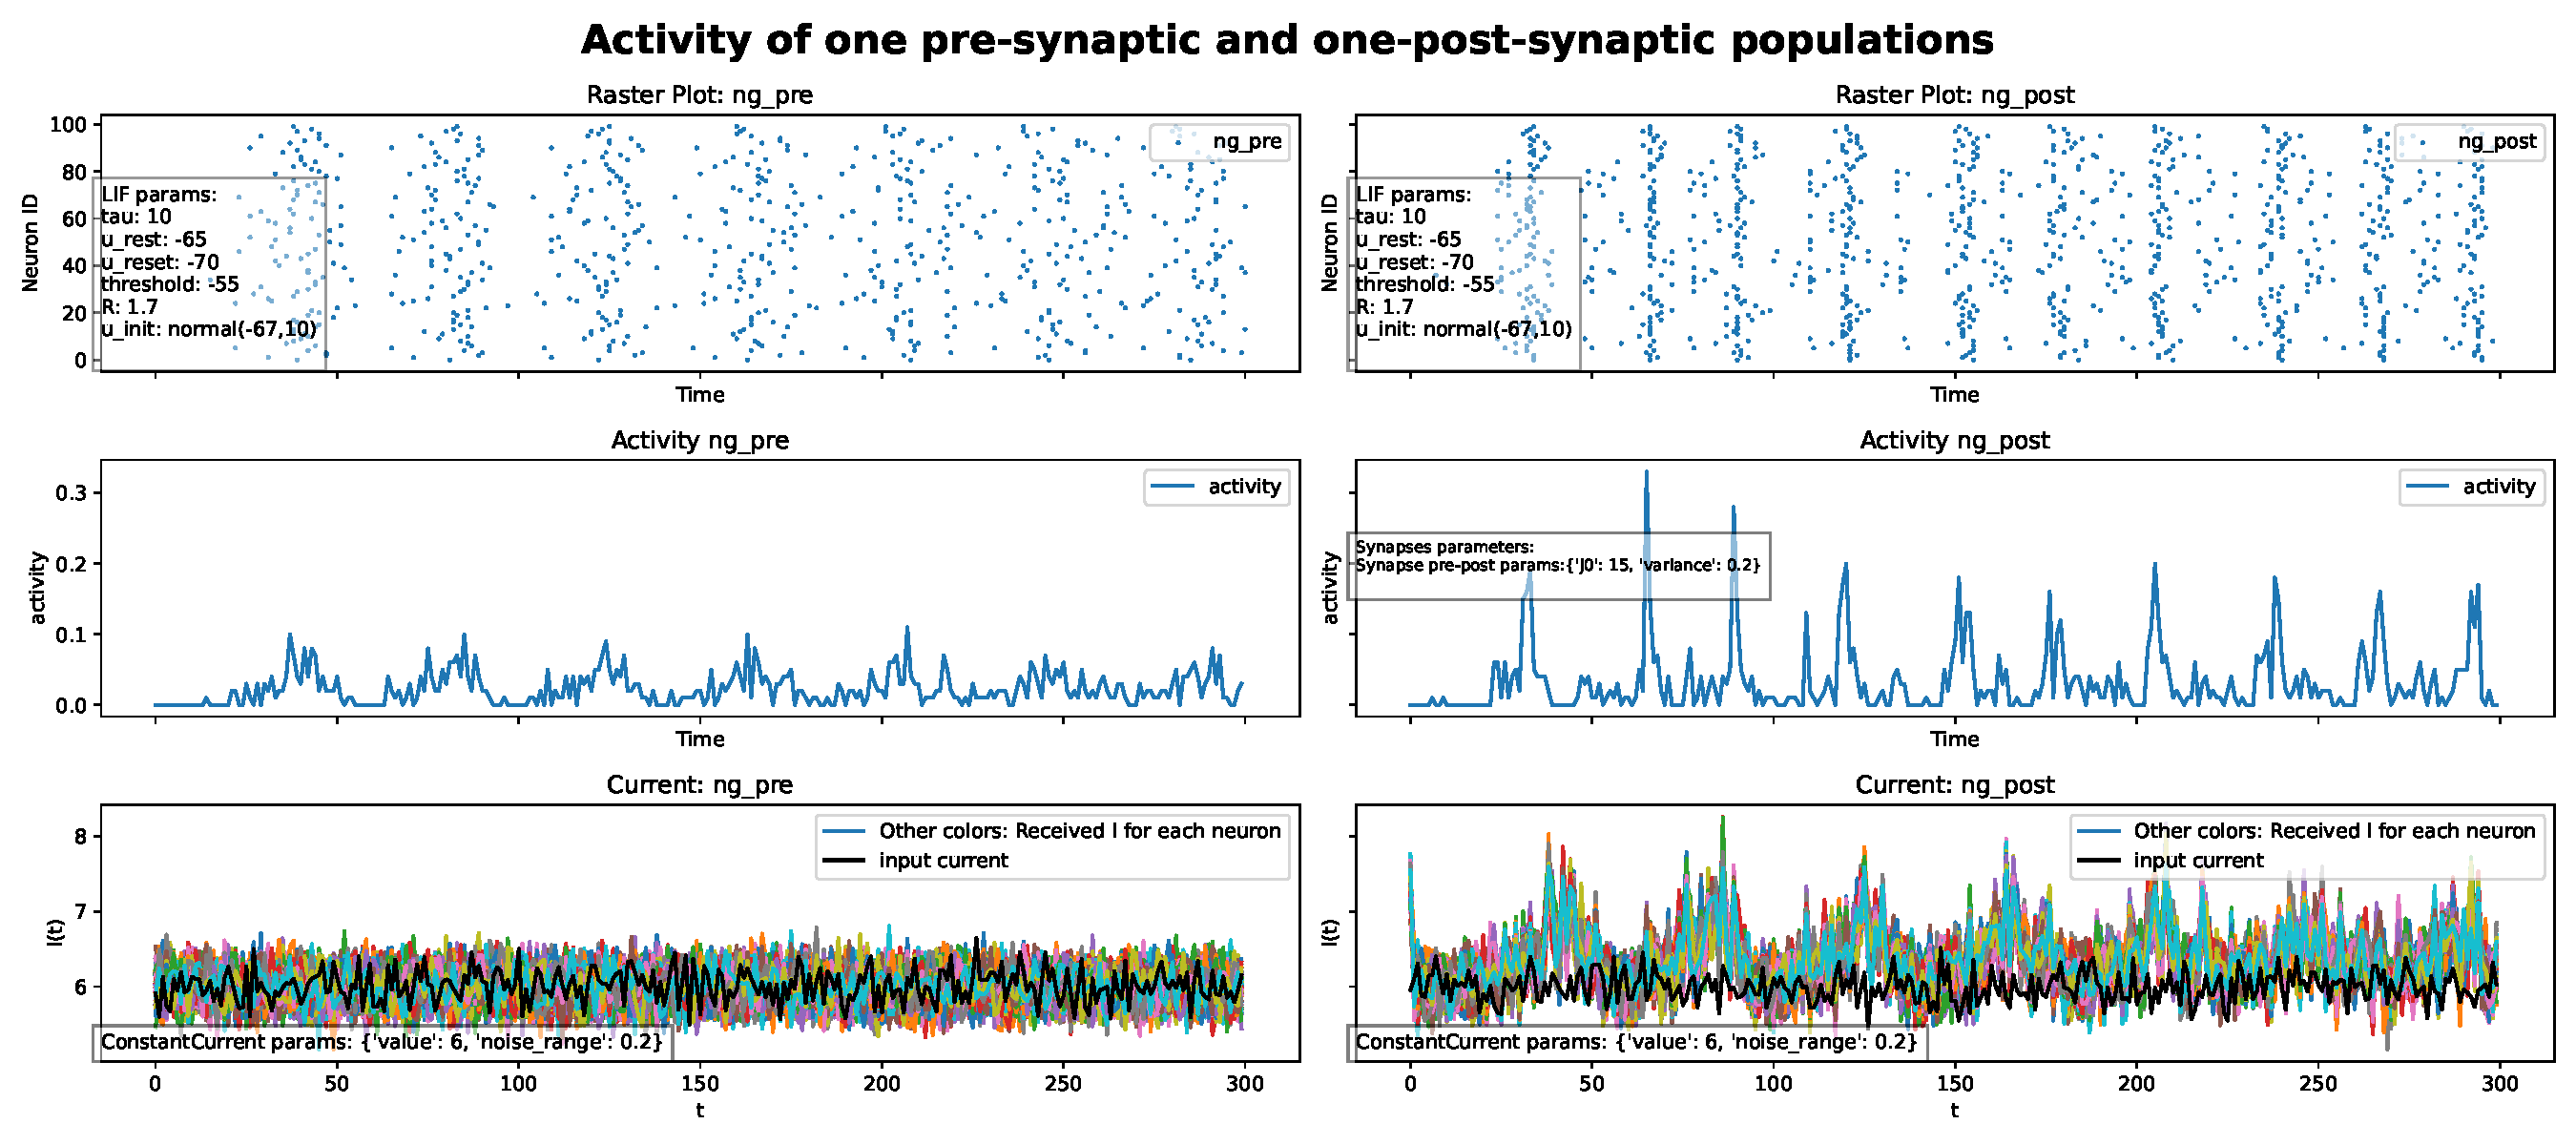
\includegraphics[width=0.9\textwidth]{plots/part1-two-ng-with-synapse-diff-curr.pdf} 
            \caption{جمعیت نورونی پیش سیناپسی و پس سیناپسی: تاثیر جریان نویزی غیریکسان}
            \label{fig:part1-two-ng-with-synapse-diff-curr}
        \end{figure}

        اگر دامنه نوسان جریان را تا 
        $0.5$ 
        بیشتر افزایش دهیم، هرچند پراکندگی زمان ضربه زدن هر دو جمعیت بیشتر می شود، ولی هنوز بیشتر بودن فعالیت جمعیت نورونی دوم مشهود است.
        (شکل \ref{fig:part1-two-ng-with-synapse-high-diff-curr})
        \begin{figure}[!ht]
            \centering
            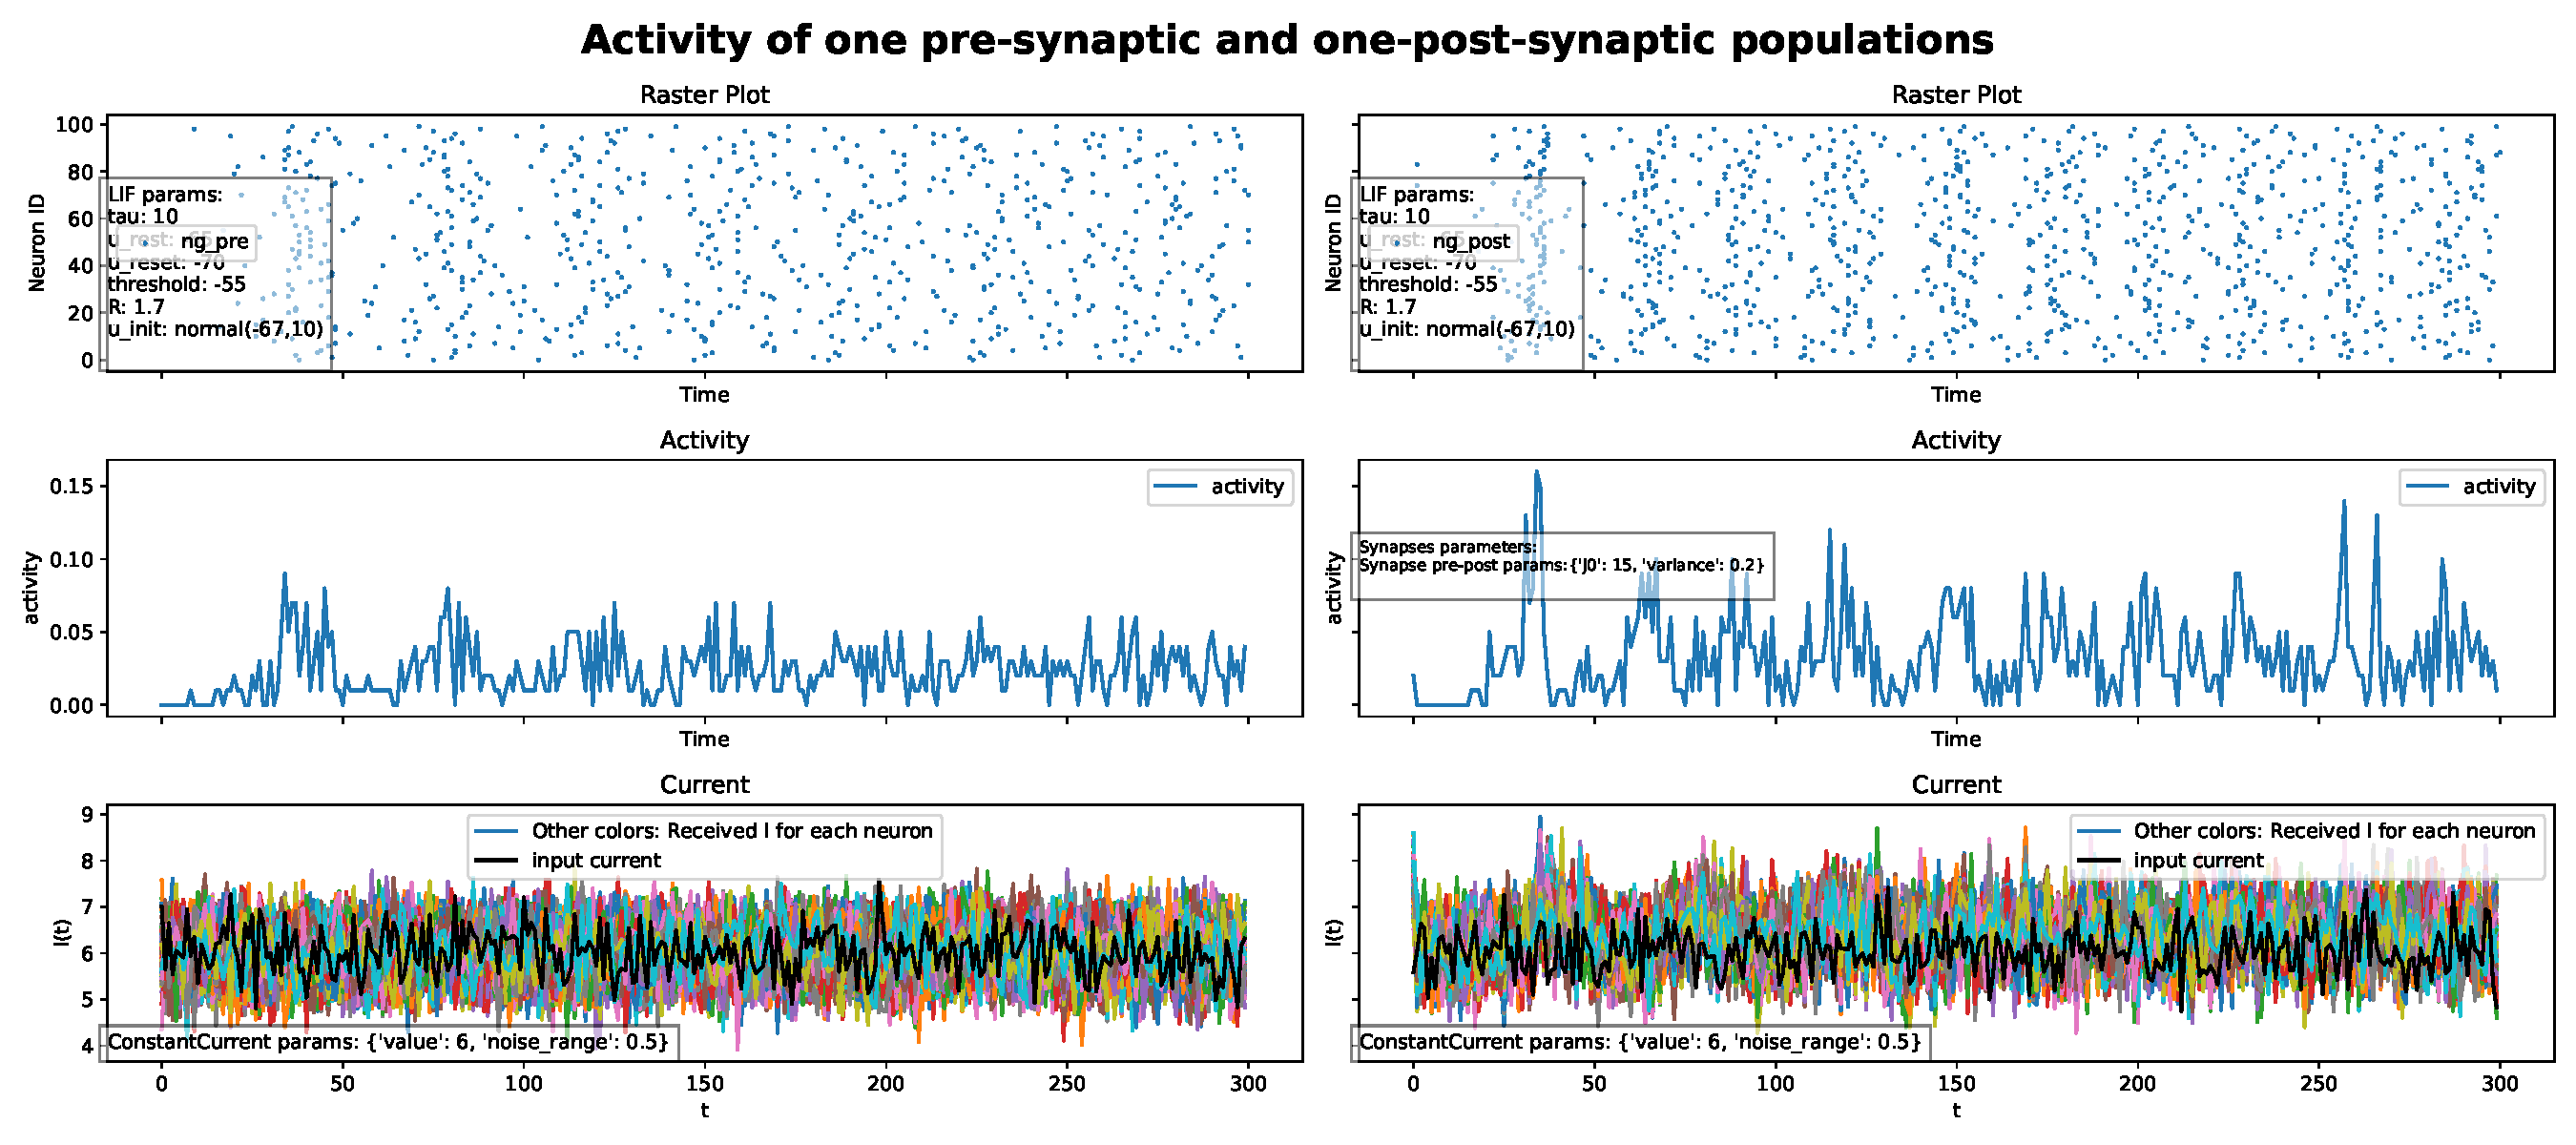
\includegraphics[width=0.9\textwidth]{plots/part1-two-ng-with-synapse-high-diff-curr.pdf} 
            \caption{جمعیت نورونی پیش سیناپسی و پس سیناپسی: تاثیر جریان نویزی غیریکسان}
            \label{fig:part1-two-ng-with-synapse-high-diff-curr}
        \end{figure}
 
        به عنوان آخرین نمودار این بخش و مقدمه ای بر بخش بعدی، افزایش مقدار 
        $j_0$ 
        را بررسی میکنیم. همانطور که از شکل 
        \ref{fig:part1-two-ng-with-synapse-high-diff-curr-high-j}
        بر می آید، افزایش 
        $j_0$ 
        منجر به افزایش وزن ها و در نتیجه افزایش جریان سیناپسی ورودی به جمعیت نورونی پس سیناپسی شده و فعالیت آن را بیشتر می کند.
        \begin{figure}[!ht]
            \centering
            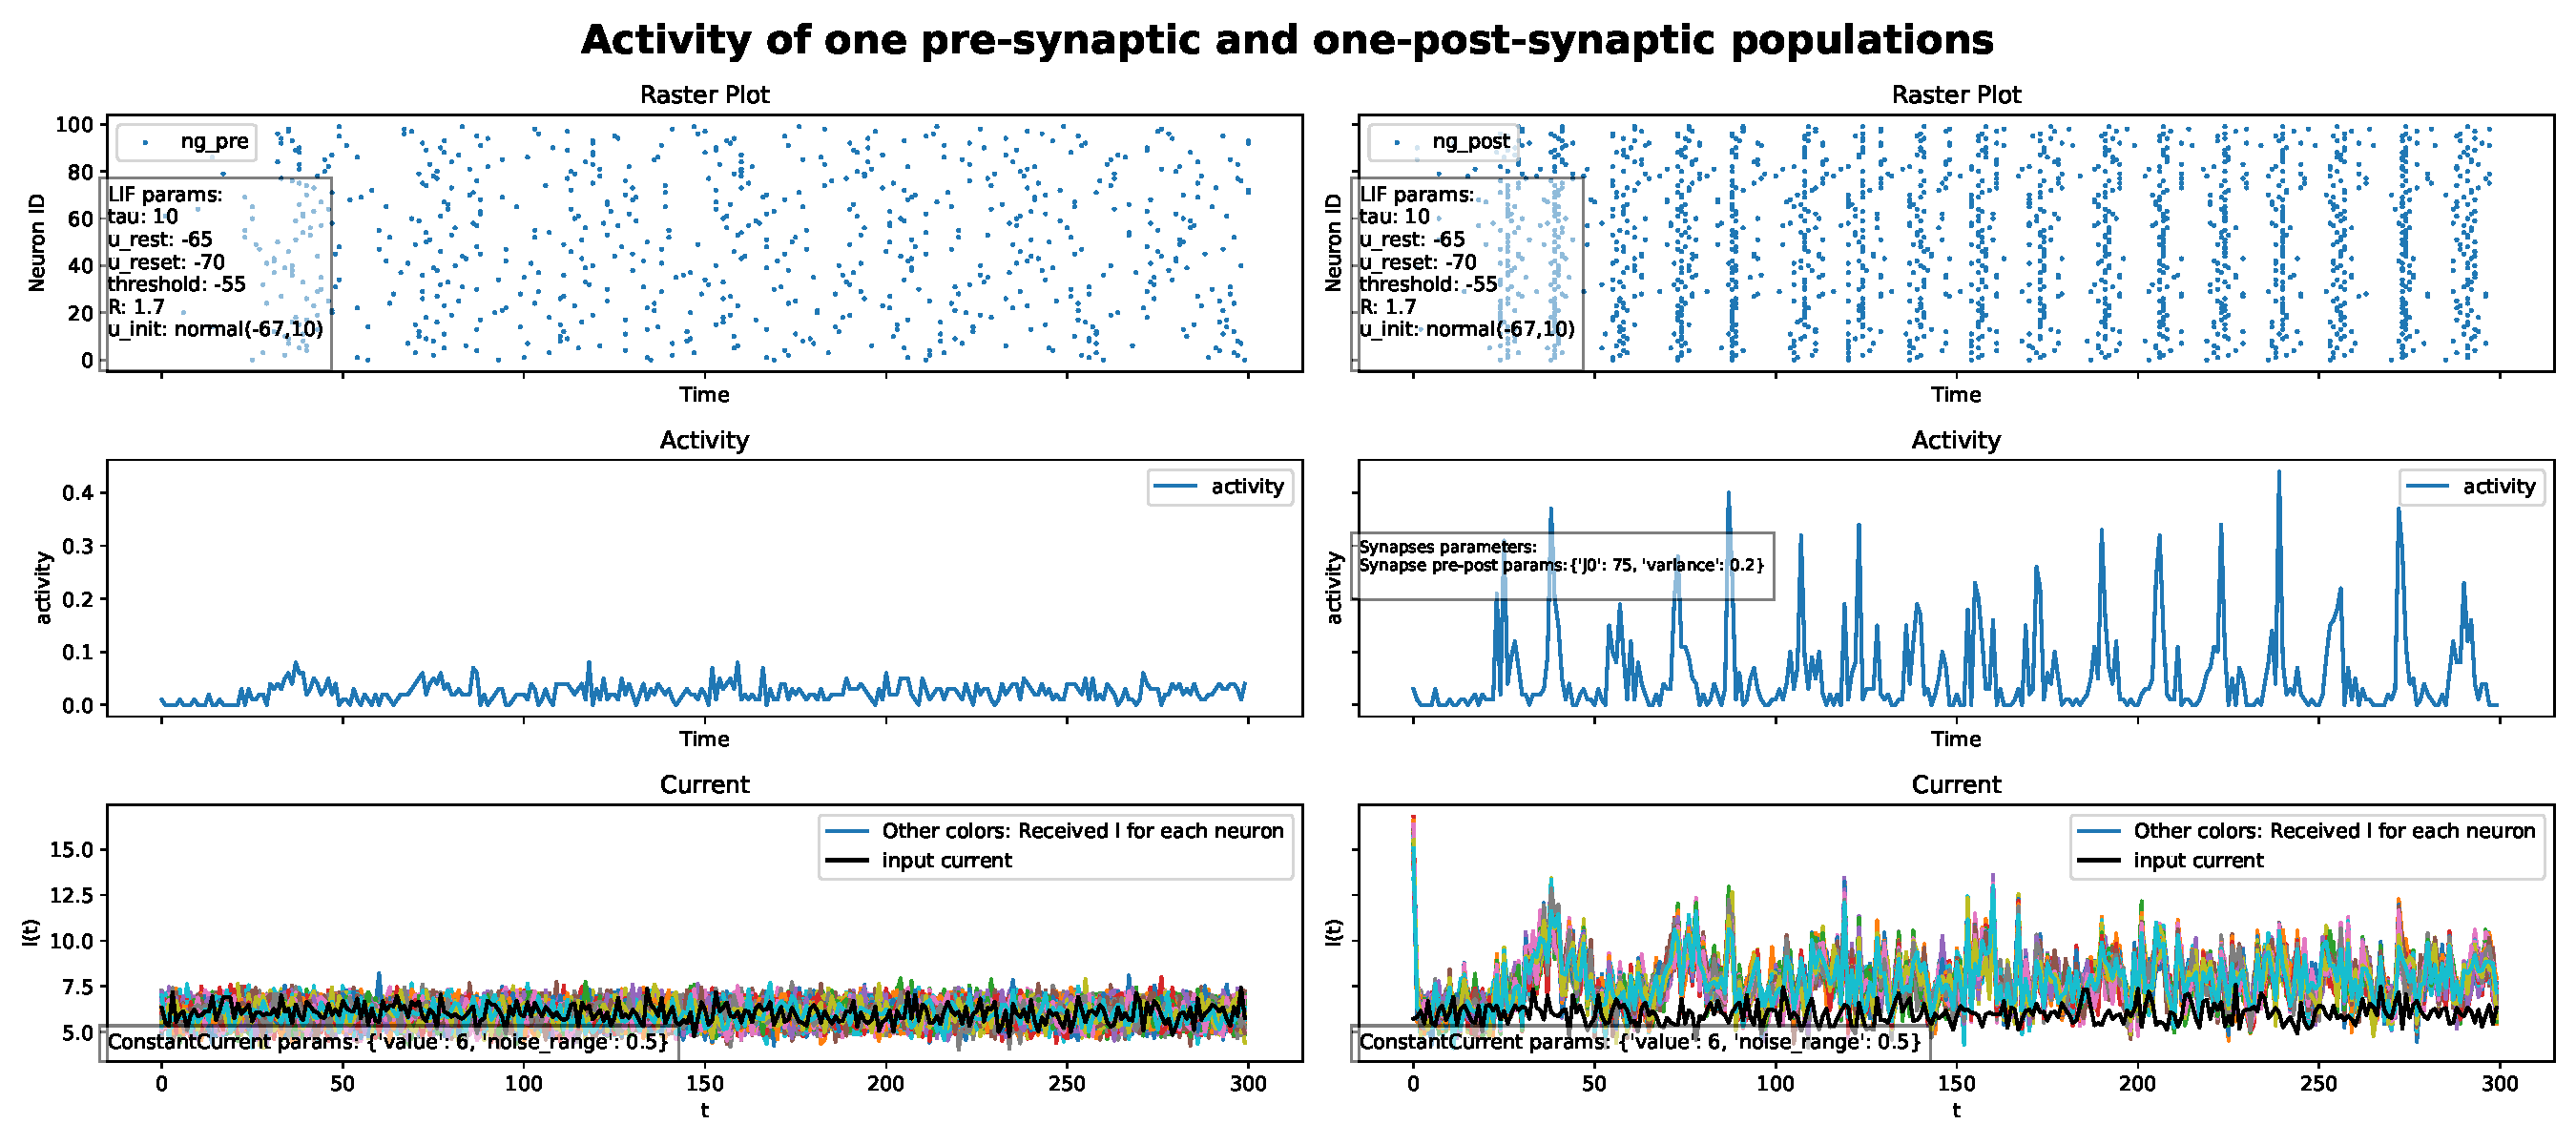
\includegraphics[width=0.9\textwidth]{plots/part1-two-ng-with-synapse-high-diff-curr-high-j.pdf} 
            \caption{جمعیت نورونی پیش سیناپسی و پس سیناپسی: تاثیر جریان نویزی غیریکسان}
            \label{fig:part1-two-ng-with-synapse-high-diff-curr-high-j}
        \end{figure}

\newpage
\section{الگو های ارتباطی}
%%%%%%%%%%%%%%%%%%%%%%%%%%% Bibliography section %%%%%%%%%%%%%%%%%%%%%%%%%%%
\newpage
\begin{thebibliography}{1}
    \bibitem{textbook}
        \begin{latin}
            Computational Neuroscience Course, School of computer science, University of Tehran
        \end{latin}
    \bibitem{PymoNNtorch}
        \begin{latin}
            PymoNNtorchPytorch-adapted version of PymoNNto
        \end{latin}
    \bibitem{wikipedia-refractory-period}
        \begin{latin}
            \href{https://en.wikipedia.org/wiki/Refractory_period_(physiology)}{Wiki-pedia: Refractory\_period\_(physiology)}
        \end{latin}
    \end{thebibliography}
\end{document}

\newpage

\section{الگو های ارتباطی}
    در این بخش از پروژه، به بررسی سه الگوی متفاوت ارتباطی، یعنی الگوی ارتباط کامل
    \footnote{\lr{Full connectivity}}، 
    ارتباط تصادفی با احتمال جفت شدن ثابت
    \footnote{\lr{Random coupling: Fixed coupling probability}}
    و ارتباط تصادفی با تعداد ثابت نورون پیش سیناپسی
    \footnote{\lr{Random coupling: Fixed number of presynaptic partners}}
    می پردازیم. در این بخش، با انجام آزمایش های مناسب، جریان حاصل و حساسیت به نویز را در هر یک از این الگو ها بررسی میکنیم.

    ارتباط واقعی بین نورون‌های قشری انواع مختلف و لایه‌های مختلف، یا درون گروه‌هایی از نورون‌های هم نوع و یک لایه هنوز تا حدی ناشناخته است، زیرا داده‌های تجربی محدود است. حداکثر، برخی برآوردهای قابل قبول از احتمالات اتصال وجود دارد. در برخی موارد احتمال اتصال به عنوان وابسته به فاصله در نظر گرفته می شود، در سایر تخمین های تجربی به عنوان یکنواخت در همسایگی محدود یک ستون
    ($column$)
    قشر مغز.
    \cite{Neuronal-Dynamics}

    در شبیه‌سازی های ما چند طرح جفت وجود دارد که اغلب مورد استفاده قرار می‌گیرند. اکثر اینها اتصال تصادفی درون و بین جمعیت ها را فرض می کنند. در ادامه این طرح‌ها را با تمرکز ویژه بر رفتار مقیاس‌بندی ناشی از هر انتخاب از طرح‌های جفت مورد بحث قرار می‌دهیم. در اینجا، رفتار مقیاس‌بندی به تغییر در تعداد 
    $N$
    نورون‌هایی که در جمعیت شرکت می‌کنند اشاره دارد.
    \cite{Neuronal-Dynamics}
    \subsection{الگوی ارتباط کامل}
        ساده ترین الگوی ارتباط، اتصال همه-به-همه در یک جمعیت است. همه اتصالات وزن یکسانی دارند. اگر بخواهیم تعداد 
        $N$
        نورون‌ها را در شبیه‌سازی یک جمعیت تغییر دهیم، یک فرمول مقیاس‌بندی مناسب، فرمول 
        $w_{ij} = \frac{j_0}{N}$
        است.

        این فرمول مقیاس‌بندی یک انتزاع ریاضی است که ما را قادر می‌سازد تا به طور فرمال حد 
        $\lim_{N\rightarrow \infty}$
        را بگیریم و در عین حال ورودی مورد انتظاری را که یک نورون از نورون های پیش سیناپسی خود در جمعیت دریافت می‌کند ثابت نگه داریم. در حد حد 
        $\lim_{N\rightarrow \infty}$
        ، نوسانات ناپدید می شوند و ورودی مورد انتظار را می توان به عنوان ورودی واقعی هر یک از نورون های 
        $N$ 
        در نظر گرفت. البته جمعیت های واقعی اندازه محدودی دارند، به طوری که همیشه برخی از نوسانات باقی می ماند. اما با افزایش 
        $N$
        نوسانات کاهش می یابد. \cite{Neuronal-Dynamics}
        
        حال به شبیه سازی و بررسی این ارتباط می پردازیم. در این قسمت، یکبار برای یک جمعیت و یکبار برای دو جمعیت، آزمایش هایمان را انجام می دهیم. از آنجا که تاثیر برخی پارامتر ها را در بخش قبل انجام دادیم، در این قسمت بیشتر روی آزمایش پارامتر های خود سیناپس ها متمرکز می شویم.
        \subsubsection{بررسی رفتار یک جمعیت}
            برای بررسی رفتار روی یک جمعیت، کافی است که یک جمعیت نورونی به همراه سیناپس داخل آن تشکیل داده و آن را شبیه سازی کنیم. از آنجا که در بخش اول، تاثیر جریان نویز دار و همچنین اختلاف پتانسیل اولیه در آورده شده است، از بررسی دوباره آن ها در اینجا خودداری می شود و پارامتر های خود سیناپس مورد تحلیل قرار میگیرد. از این رو، 
            برای شروع، یک جمعیت نورونی با مدل 
            $LIF$
            (\lr{Leaky-integrate-and-fire})
            \footnote{مدل تجمیع و آتش نشتی}
            با پارامتر های 
            $\tau=10$,
            $u_{rest}=-65$,
            $u_{reset}=-70$,
            $threshold=-55$,
            $R=1.7$,
            $u_{init}=normal(-67,10)$
            و جریان ثابت نویزدار
            $6$ 
            میسازیم. 
            \paragraph{پارامتر $j_0$}
                در ابتدا تاثیر پارامتر 
                $j_0$
                را بر روی رفتار تحلیل میکنیم. برای این منظور، سه مقدار 
                $j_0=5$,
                $j_0=25$,
                $j_0=75$
                را شبیه سازی میکنیم. همچنین پارامتر واریانس را 
                $\tilde{\sigma}=0.25$ 
                میگیریم. از آنجا که فرمول موردنیاز برای واریانس به طور کامل برای هر سه مدل شرح داده نشده بود، به طور کلی برای سه مدل، این پارامتر در مقدار میانگین نهایی
                (فرمول $\frac{j_0}{N}$) 
                ضرب شده و مقدار واریانس در توزیع 
                $normal(\mu,\sigma)$ 
                را می سازد.
                % \begin{equation}
                %     w_{ij}=normal(\mu,\sigma); \mu=\frac{j0}{N}, \sigma=\mu\times\tilde{\sigma}
                % \end{equation}
                همانطور که در شکل 
                \ref{fig:part2-one-ng-full-synapse-diff-j}
                مشاهده میکنیم، با افزایش 
                $j_0$ 
                میزان نواسات کاهش می یابد. تحلیل من از این اتفاق این است که با زیاد شدن مقدار وزن های سیناپسی در یک جمعیت نورونی، بعد از ضربه زدن نورون های یک جمعیت، مقدار جریان حاصل از سیناپس نیز افزایش یافته، و در لحظه بعدی نورون ها جریان بیشتری دریافت کرده و در نتیجه سریع تر ضربه میزنند. از آنجا که سرعت ضربه زدن آن ها افزایش می یابد، تفاوت اختلاف پتانسیل متفاوتی که در مقدار دهی اولیه به آن ها داده شده بود نیز رفته رفته کمتر شده و پس از مدتی زمان ضربه زدن نورون ها نزدیک به یکدیگر می شود. علاوه بر کم شدن پراکندگی لحظات ضربه ها، میبینم که در نمودار سمت راست، نورون ها تعداد ضربه های بیشتری نیز در کل زده اند.
                \begin{figure}[!ht]
                    \centering
                    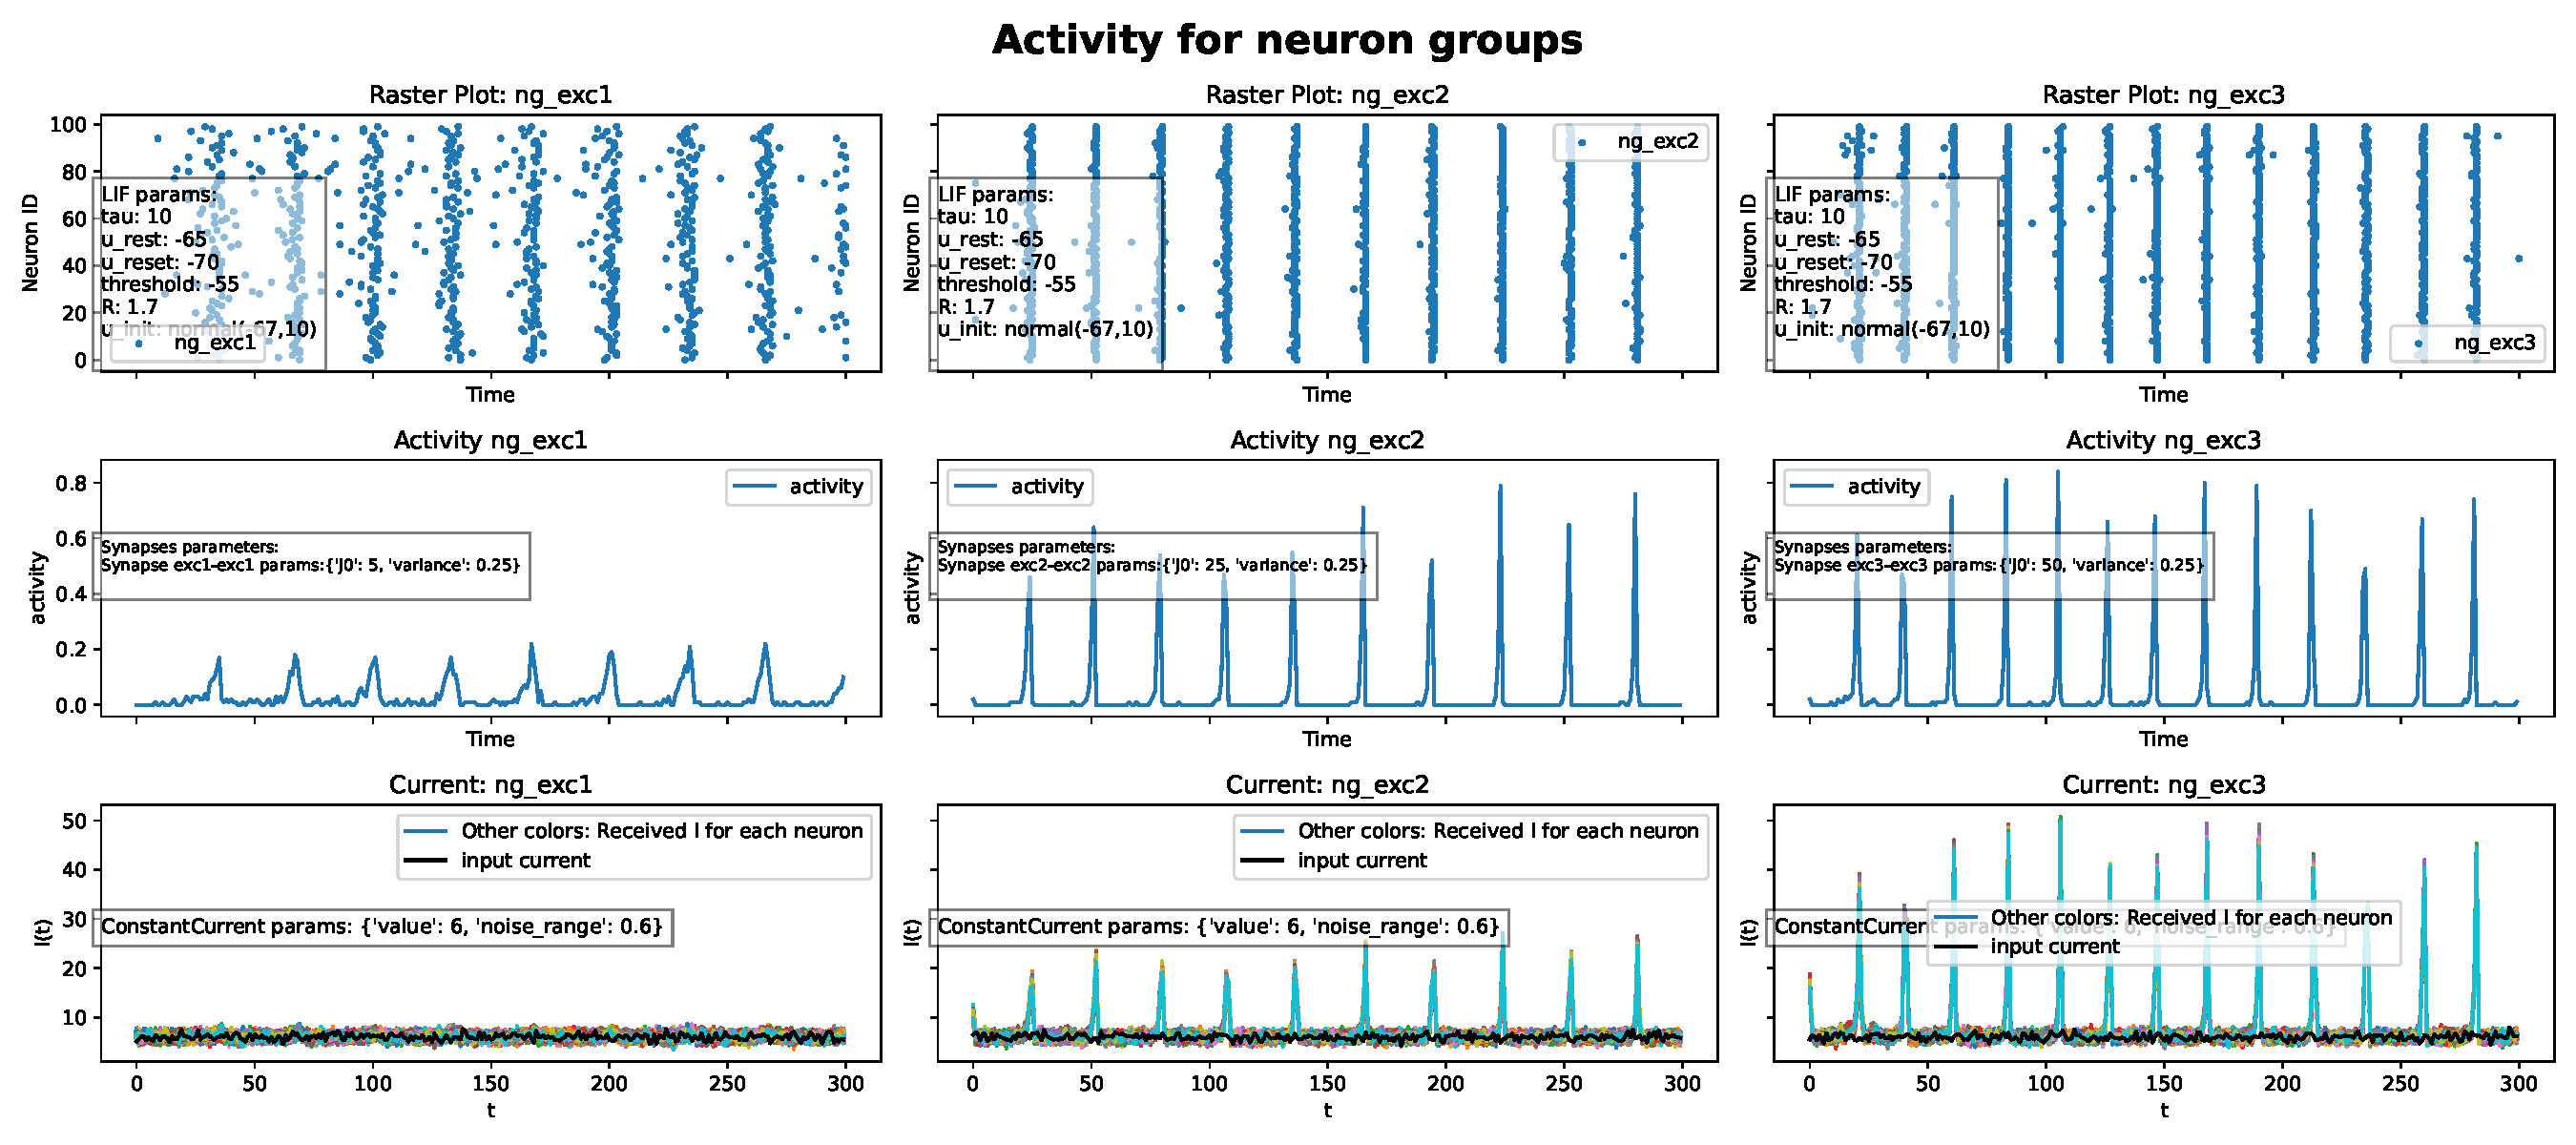
\includegraphics[width=0.9\textwidth]{plots/part2-one-ng-full-synapse-diff-j.pdf} 
                    \caption{رفتار یک جمعیت نورونی با مقادیر $j_0$ مختلف و جریان ثابت نویز دار}
                    \label{fig:part2-one-ng-full-synapse-diff-j}
                \end{figure}

                حال به جمعیت نورونی مان، یک جریان تصادفی میدهیم تا رفتار شبیه به نورون واقعی را بیشتر بررسی کنیم. مجددا در شکل
                \ref{fig:part2-one-ng-full-synapse-diff-j-rand-curr}
                مشاهده میکنیم که تصادفی بودن جریان، منجر به پراکندگی زمان ضربه زدن نورون ها می شود و به طور کلی فعالیت آن ها را کاهش داده است، اما با زیاد کردن وزن های سیناپسی، این نوسانات کمتر شده به طور که در نمودار سمت راست، میتوانیم زمان ضربه زدن نورون ها را در ستون هایی دسته بندی کنیم.
                \begin{figure}[!ht]
                    \centering
                    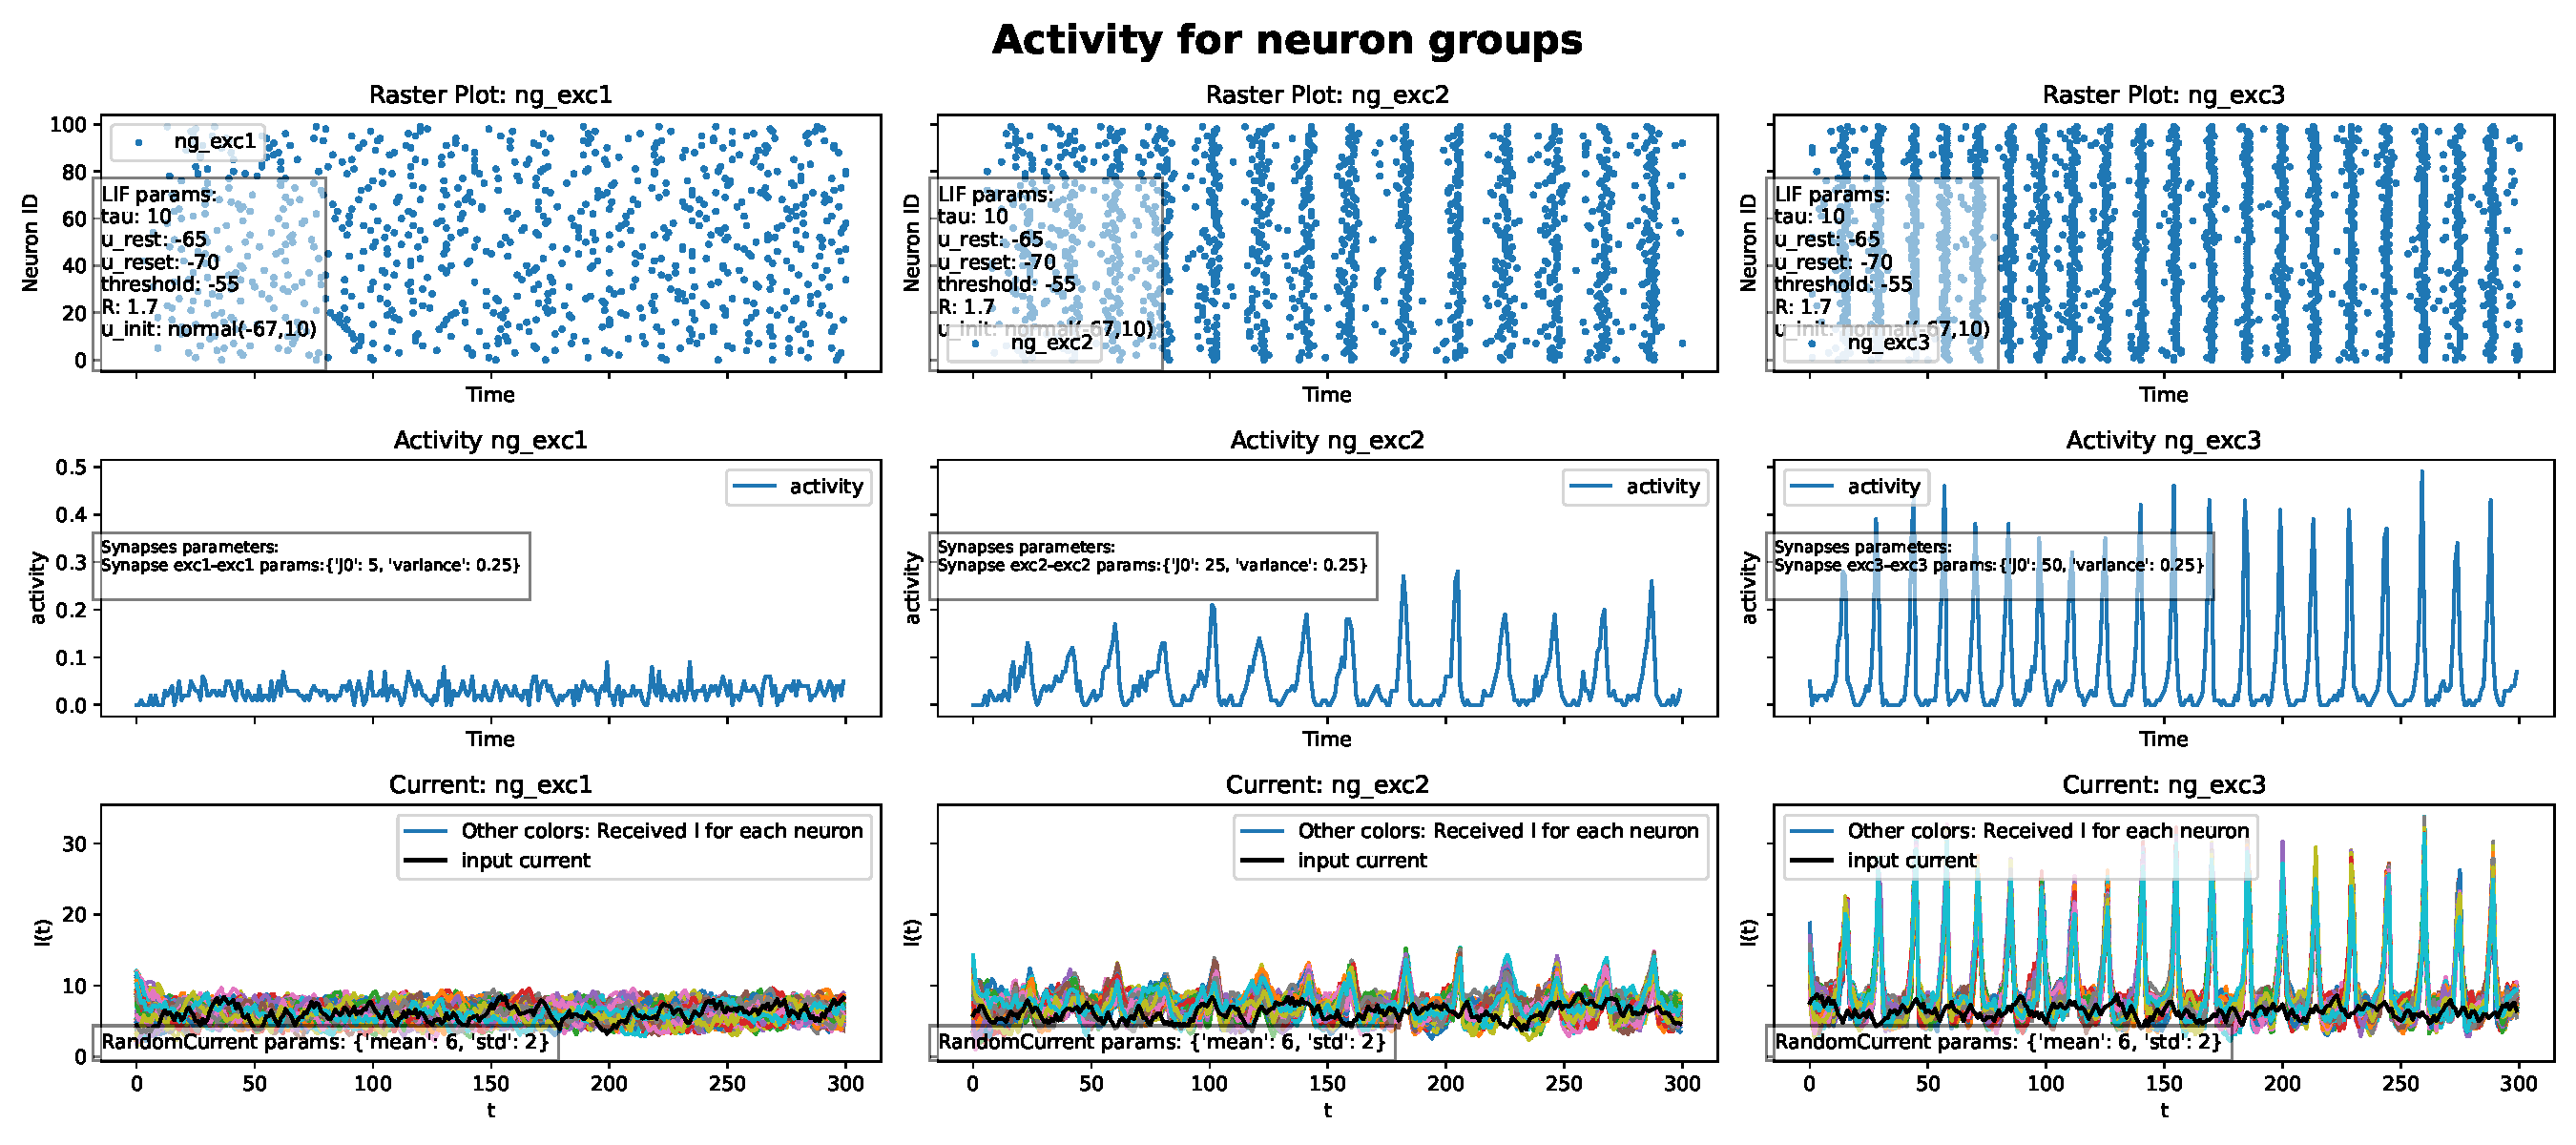
\includegraphics[width=0.9\textwidth]{plots/part2-one-ng-full-synapse-diff-j-rand-curr.pdf} 
                    \caption{رفتار یک جمعیت نورونی با مقادیر $j_0$ مختلف و جریان تصادفی}
                    \label{fig:part2-one-ng-full-synapse-diff-j-rand-curr}
                \end{figure}

            \paragraph*{پارامتر واریانس}
                حال رفتار جمعیت را به ازای مقادیر مختلف واریانس تحلیل میکنیم. برای این قسمت نیز از همان مدل نورونی بالا استفاده میکنیم. از آنجا که الگوی ارتباطی مان کامل است، انتظار داریم که تغییر معقول واریانس تفاوت زیادی در رفتار کلی نورون ها ایجاد نکند، چرا که هر نورون با تمام نورون های دیگر ارتباط دارد و از این رو برآیند جریان سناپسی وارد شده به نورون ها نزدیک به هم می باشد. شکل 
                \ref{fig:part2-one-ng-full-synapse-diff-variance}
                بیانگر همین موضوع است. هر چند تغییرات کوچکی میتواند رخ دهد. مثلا در نمودار سمت راست که واریانس برابر با خود میانگین دارد
                (گفتیم که عددی که به عنوان واریانس به مدل ورودی داده می شود در میانگین ضرب شده و سپس تشکیل واریانس اصلی توزیع را می دهد)،
                میزان فعالیت کلی نورون ها کمی از دو مدل دیگر بیشتر است.
                \begin{figure}[!ht]
                    \centering
                    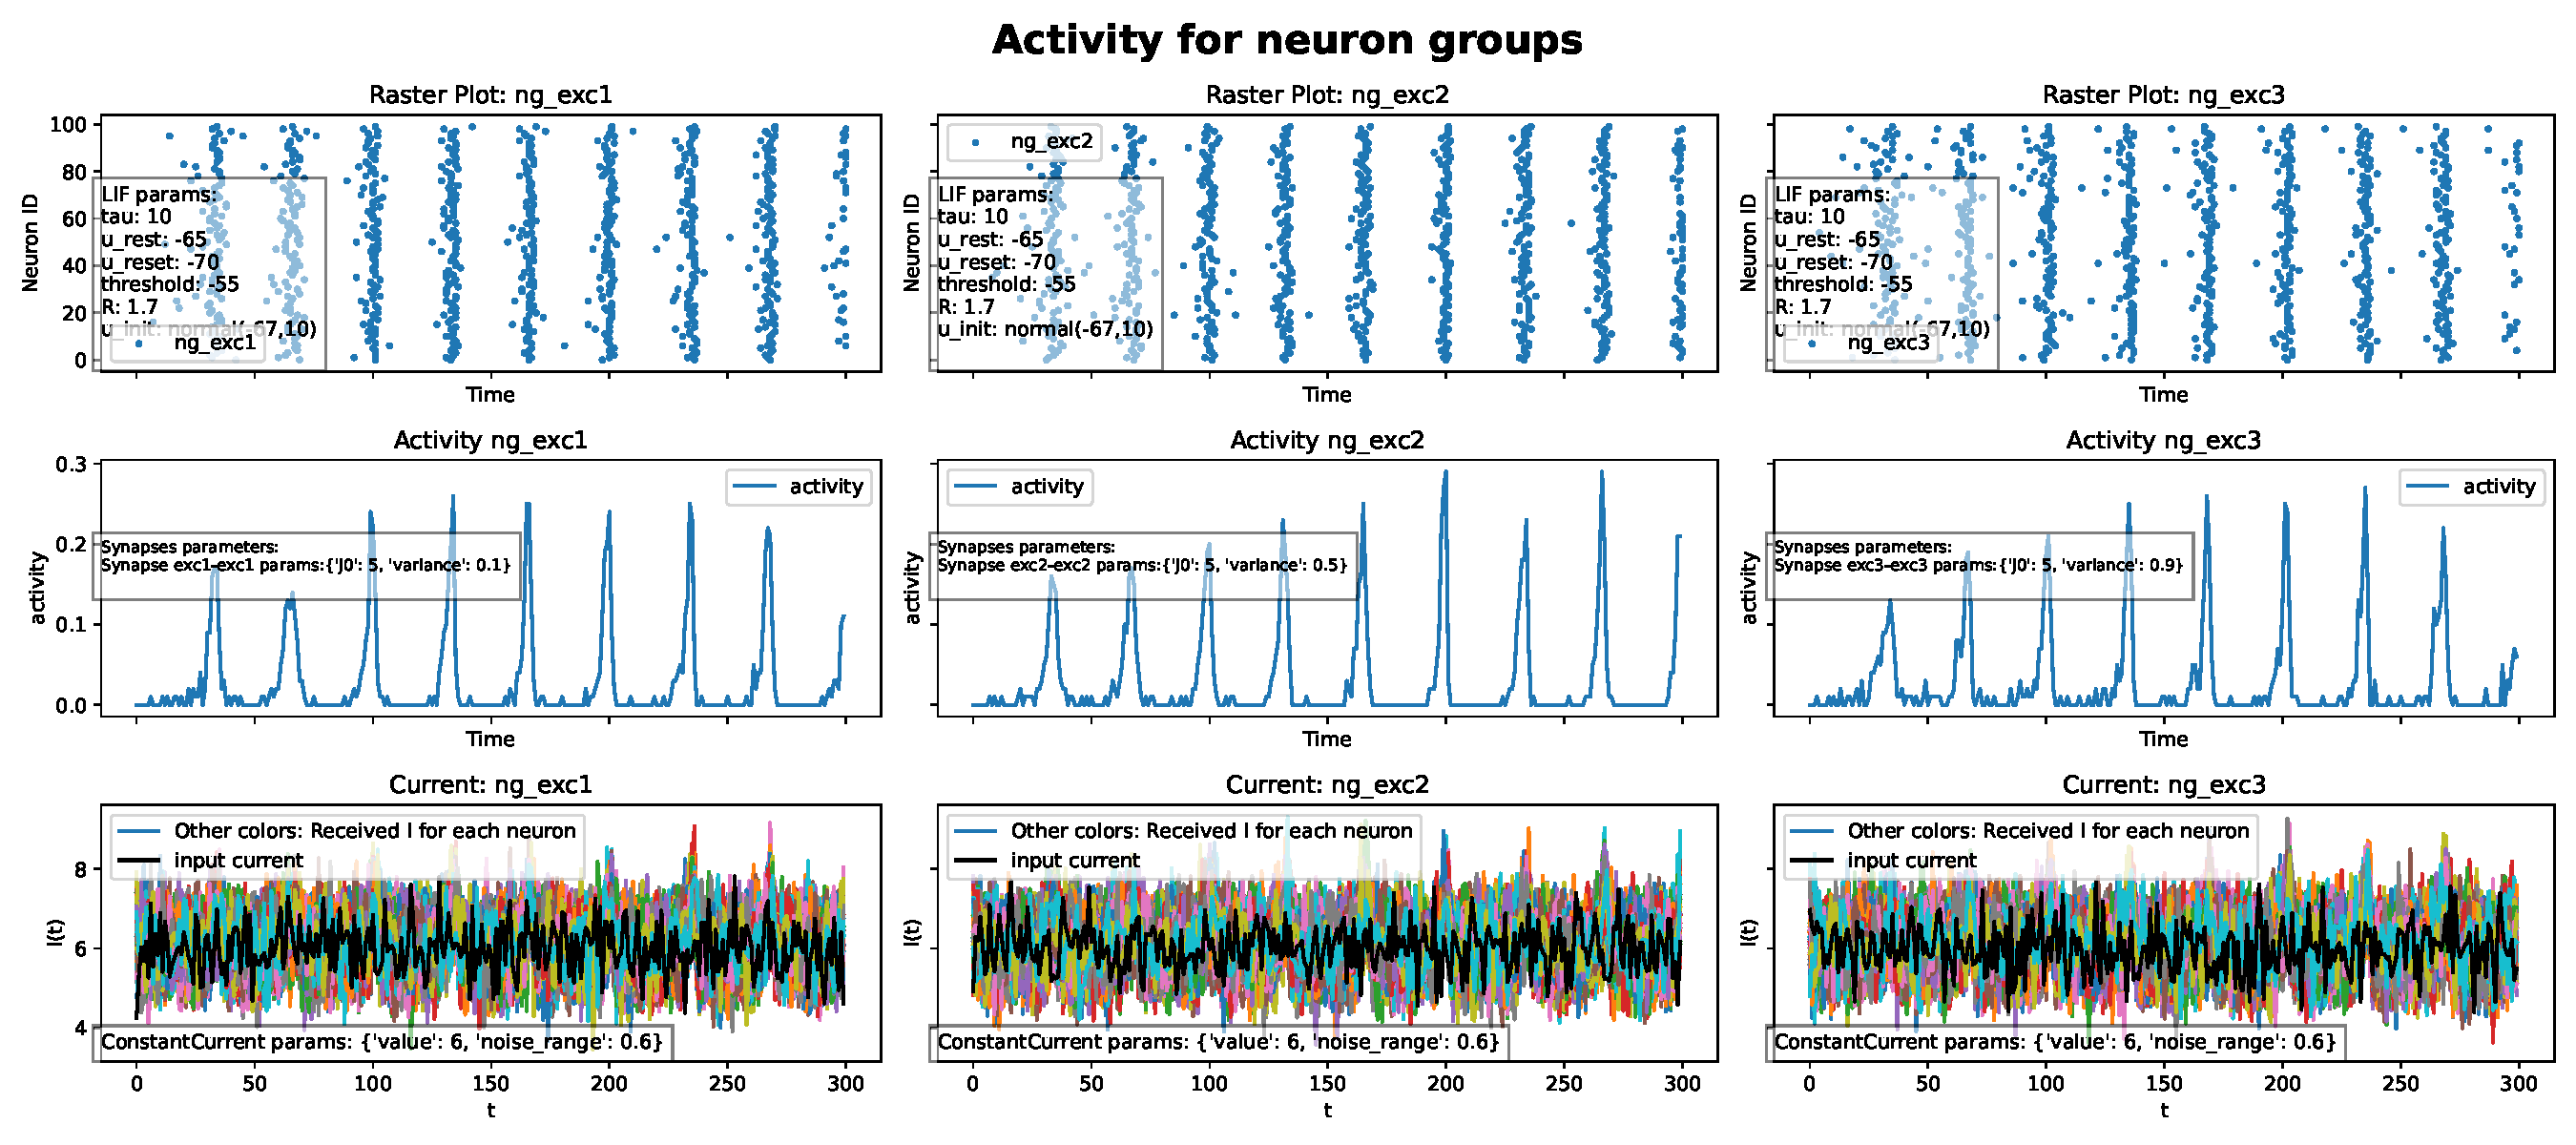
\includegraphics[width=0.9\textwidth]{plots/part2-one-ng-full-synapse-diff-variance.pdf} 
                    \caption{رفتار یک جمعیت نورونی با واریانس مختلف و جریان ثابت نویزدار}
                    \label{fig:part2-one-ng-full-synapse-diff-variance}
                \end{figure}

                حال رفتار را با یک جریان تصادفی آزمایش می کنیم. در جریان تصادفی نیز مطابق شکل
                \ref{fig:part2-one-ng-full-synapse-diff-variance-rand-curr}
                دریافت می شود که تغییر واریانس تاثیر چندانی بر روی رفتار جمعیت ندارد. به طور کلی میتوان این نتیجه را گرفت که در الگوی ارتباط کامل با جریان غیر ثابت، به دلیل اینکه همه نورون ها با یکدیگر در ارتباط هستند، افزودن واریانس به وزن ها نمیتواند روی جریان تصادفی تاثیر بگذارد.

                \begin{figure}[!ht]
                    \centering
                    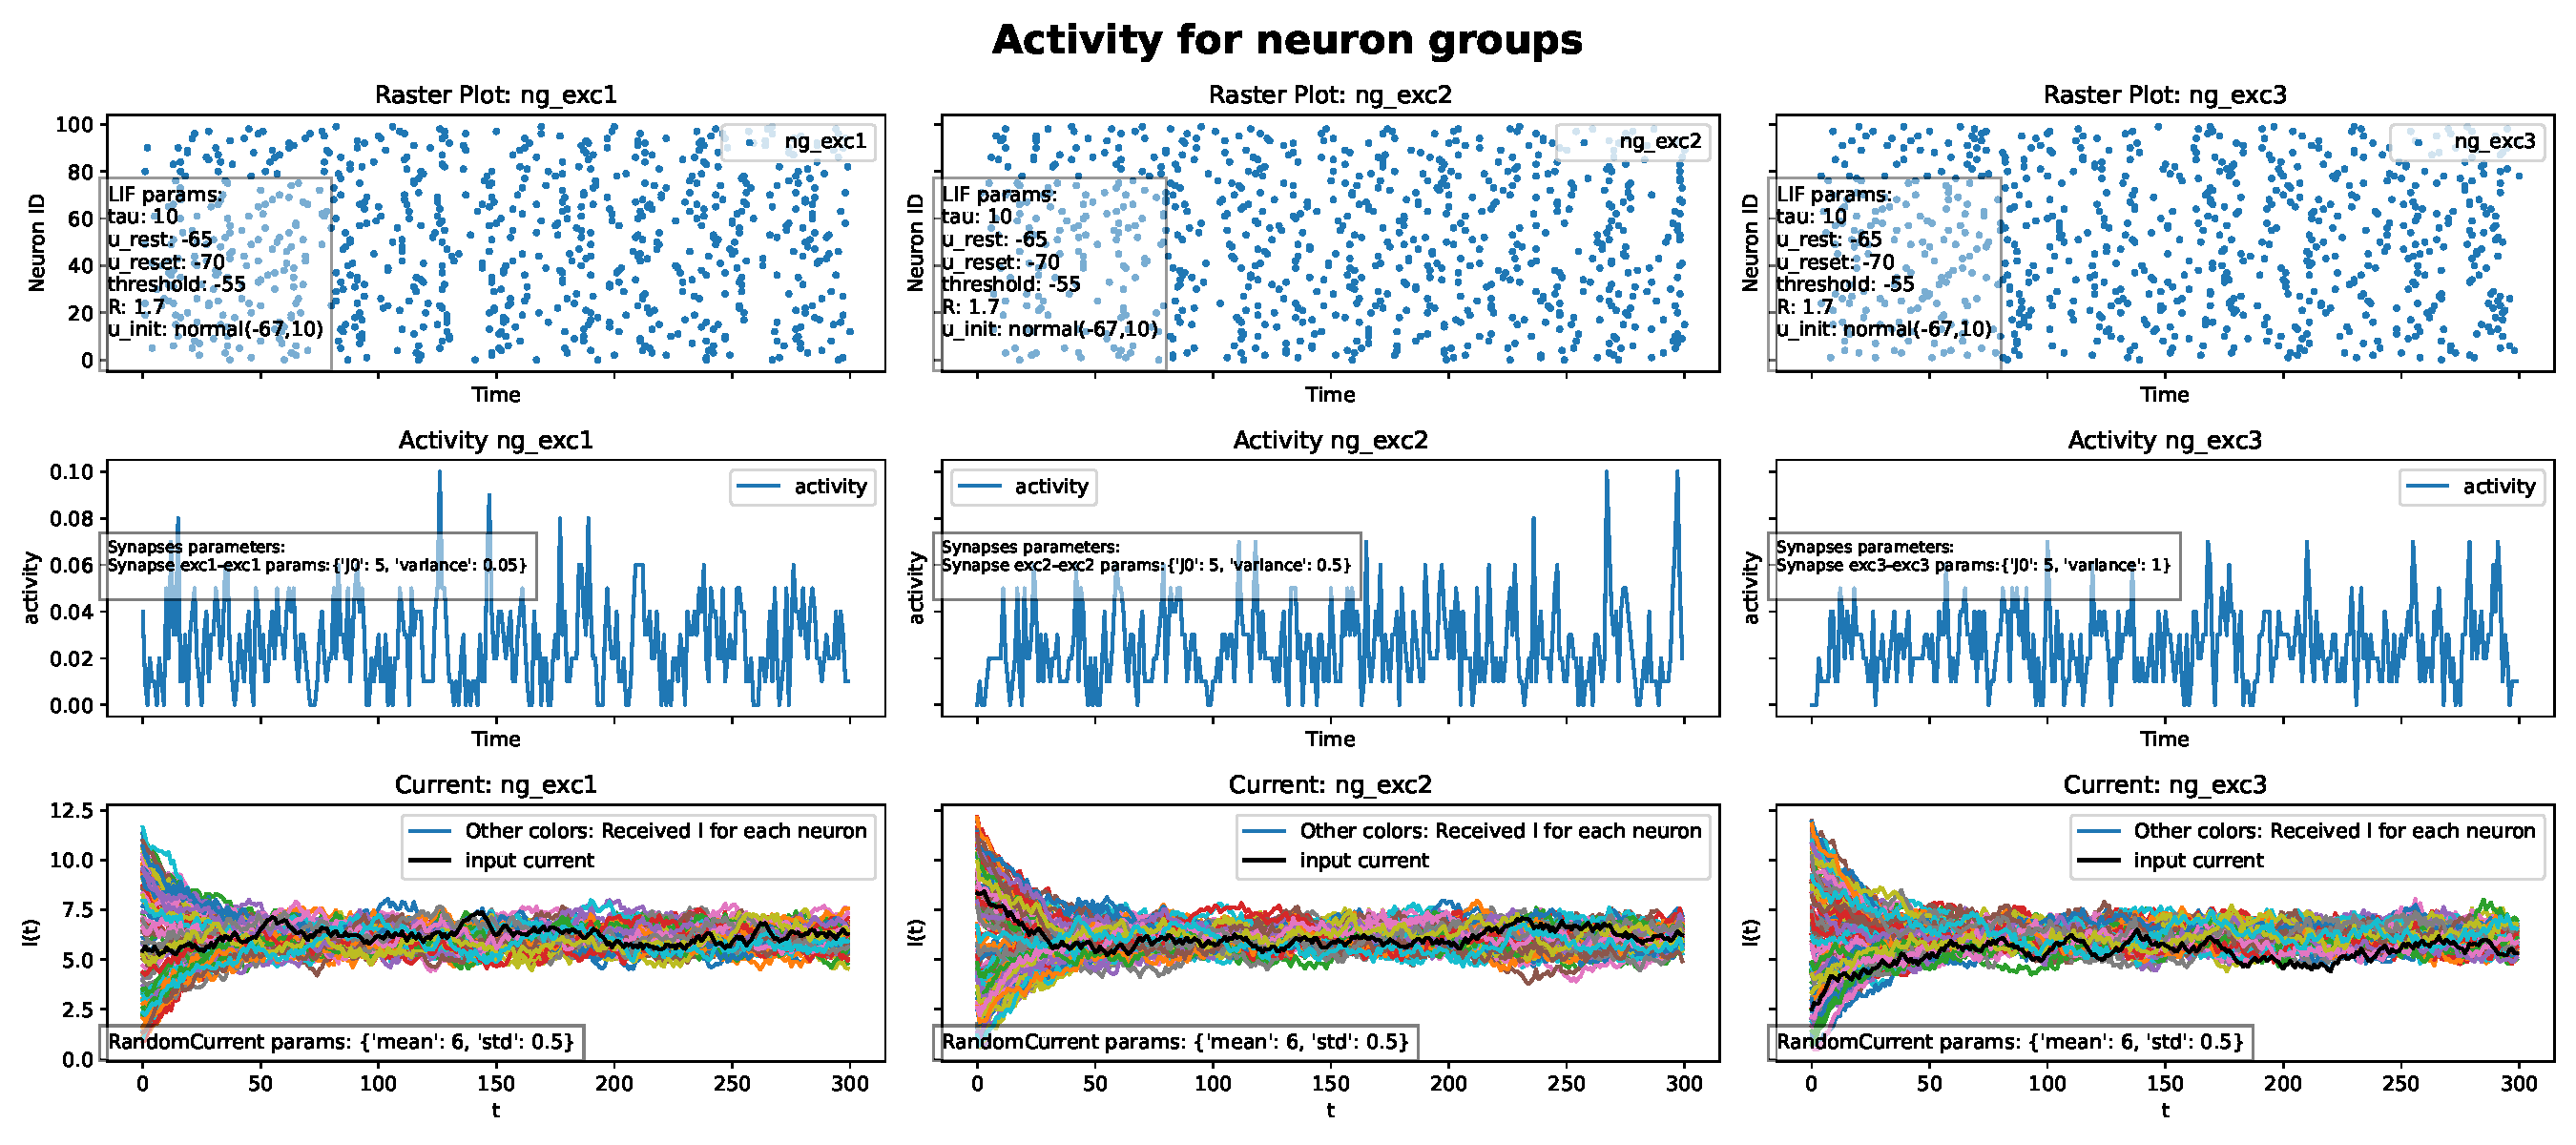
\includegraphics[width=0.9\textwidth]{plots/part2-one-ng-full-synapse-diff-variance-rand-curr.pdf} 
                    \caption{رفتار یک جمعیت نورونی با واریانس مختلف و جریان تصادفی}
                    \label{fig:part2-one-ng-full-synapse-diff-variance-rand-curr}
                \end{figure}

            \paragraph*{اندازه جمعیت}
                خالی از لطف نیست که تاثیر اندازه جمعیت را روی رفتار آن بررسی میکنیم. برای اینکار سه جمعیت نورونی به اندازه های ۵۰، ۱۰۰ و ۲۵۰ را بررسی میکنیم تا ببینیم اندازه چه تاثیری روی رفتار جمعیت دارد. طبق شکل
                \ref{fig:part2-one-ng-full-synapse-diff-size}
                مشاهده می کنیم که اگر مدل نورون ها و جریان را یکی بگیریم، برای جمعیت با اندازه های متفاوت، فعالیت نورونی تغییری نکرده و مستقل از اندازه جمعیت است.
                \begin{figure}[!ht]
                    \centering
                    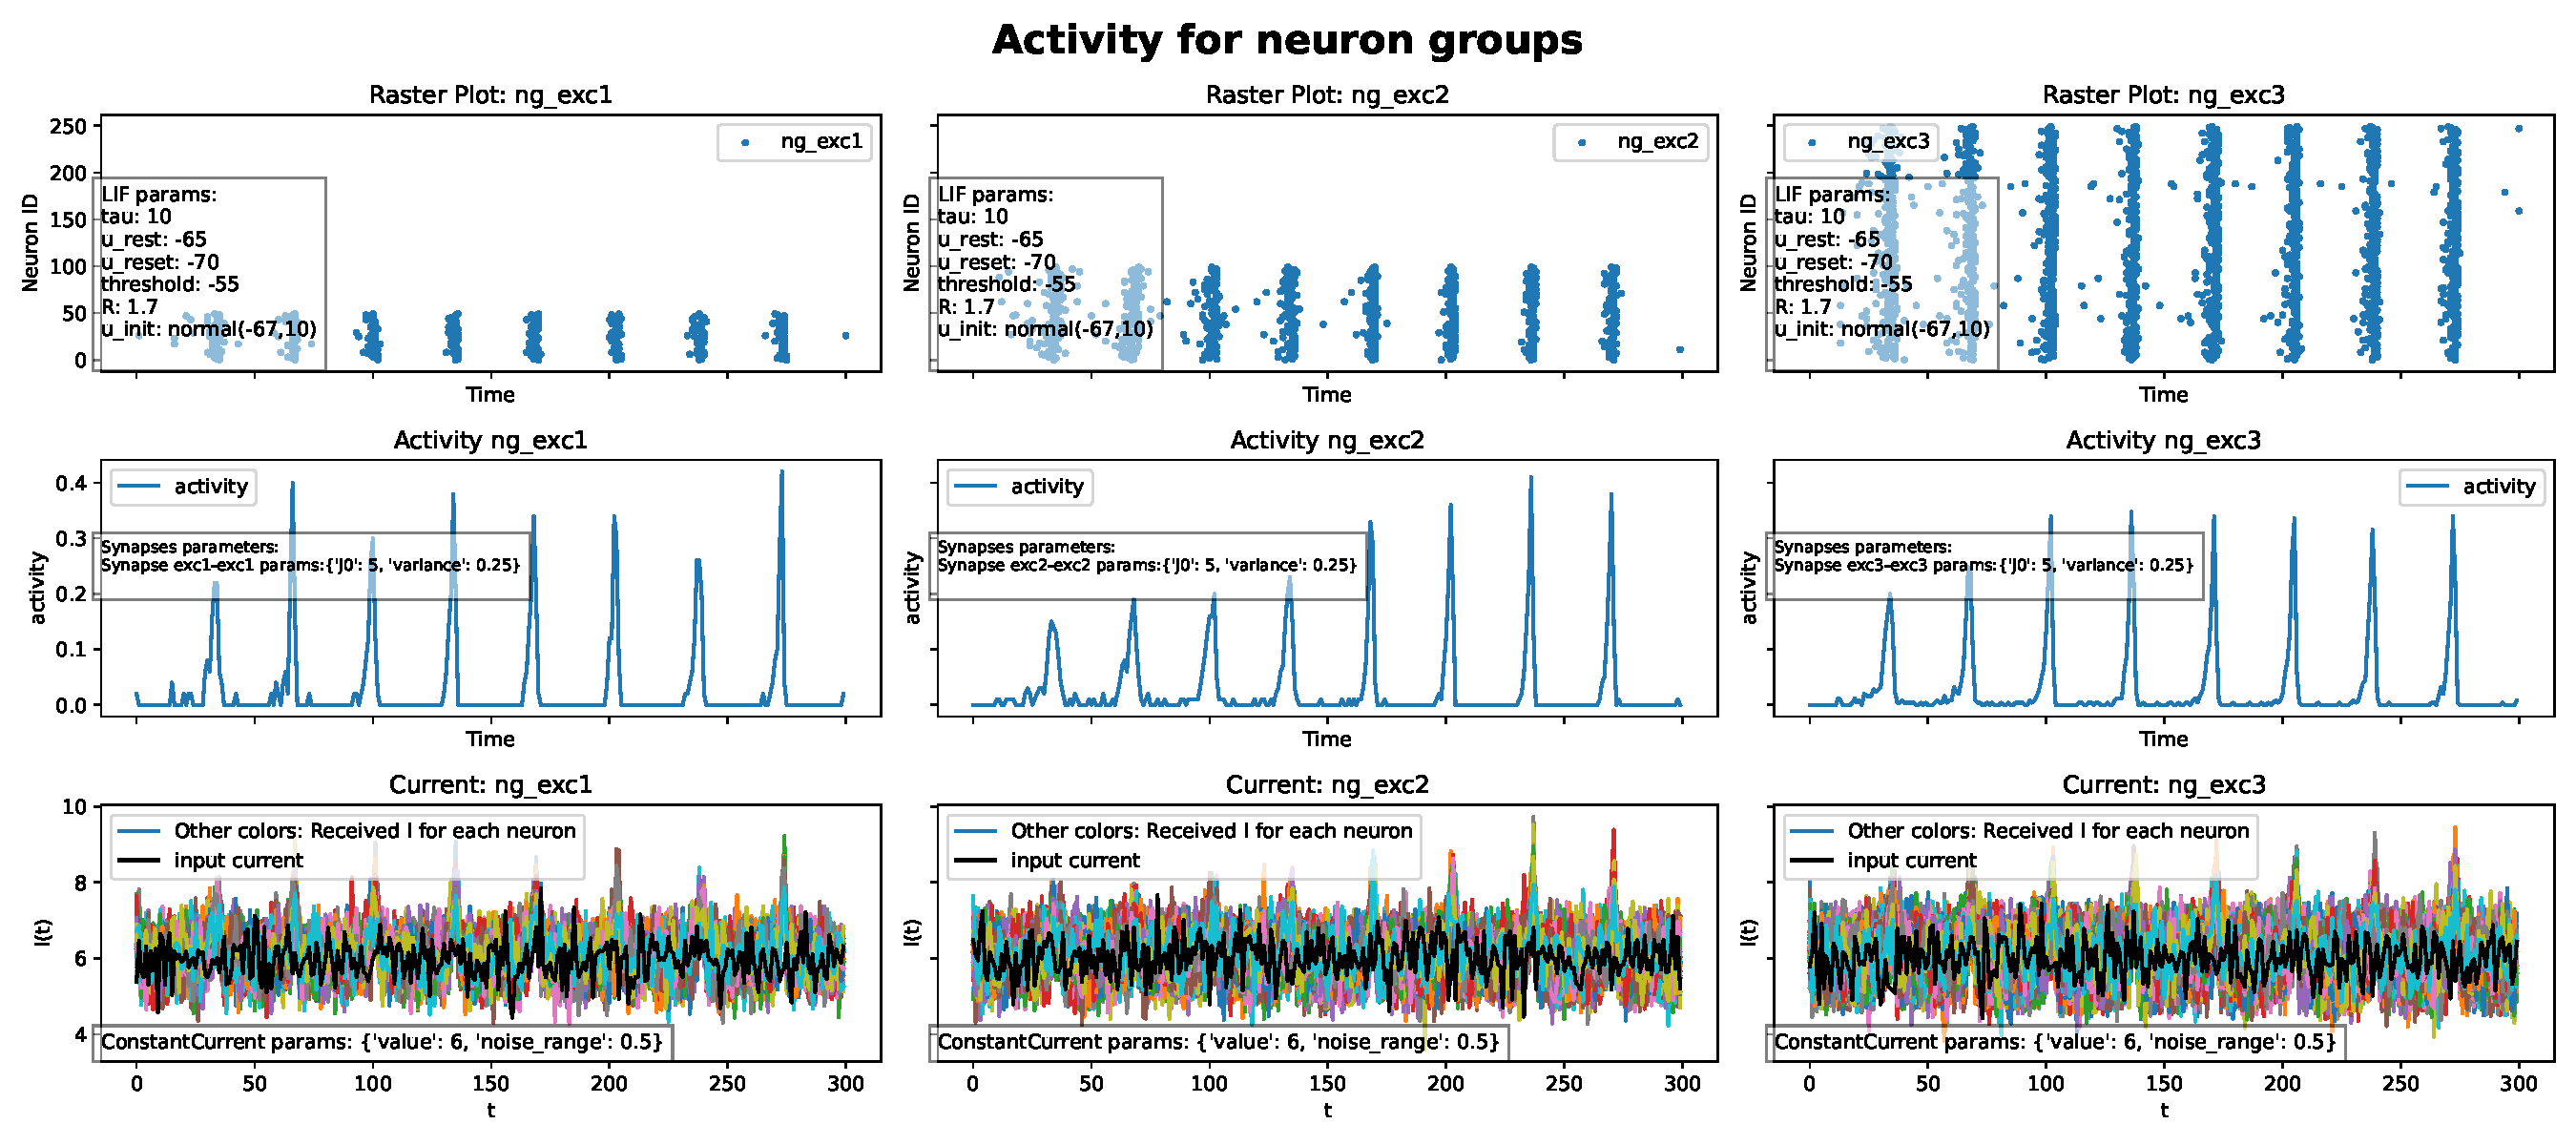
\includegraphics[width=0.9\textwidth]{plots/part2-one-ng-full-synapse-diff-size.pdf} 
                    \caption{رفتار یک جمعیت نورونی با جمعیت مختلف و جریان تصادفی}
                    \label{fig:part2-one-ng-full-synapse-diff-size}
                \end{figure}
            \paragraph*{مدل های نورونی}
                در نهایت نیز به سراغ بررسی تاثیر انتخاب مدل نورونی روی رفتار جمعیت میرویم. همانطور که از شکل
                \ref{fig:part2-one-ng-full-synapse-diff-neuron-model}
                پیداست، رفتار مدل نورونی 
                $LIF$ و
                $ELIF$ 
                شبیه یکدیگر است در حالی که در مدل 
                $AELIF$ 
                با گذر زمان، فعالیت نورونی کاهش یافته و به مقدار کمتری همگرا می شود. هر چند من خیلی هنگام پیاده سازی روی قسمت های ۲ مدل دیگر مانور ندادم و ممکن است دقیق نباشند.
                \begin{figure}[!ht]
                    \centering
                    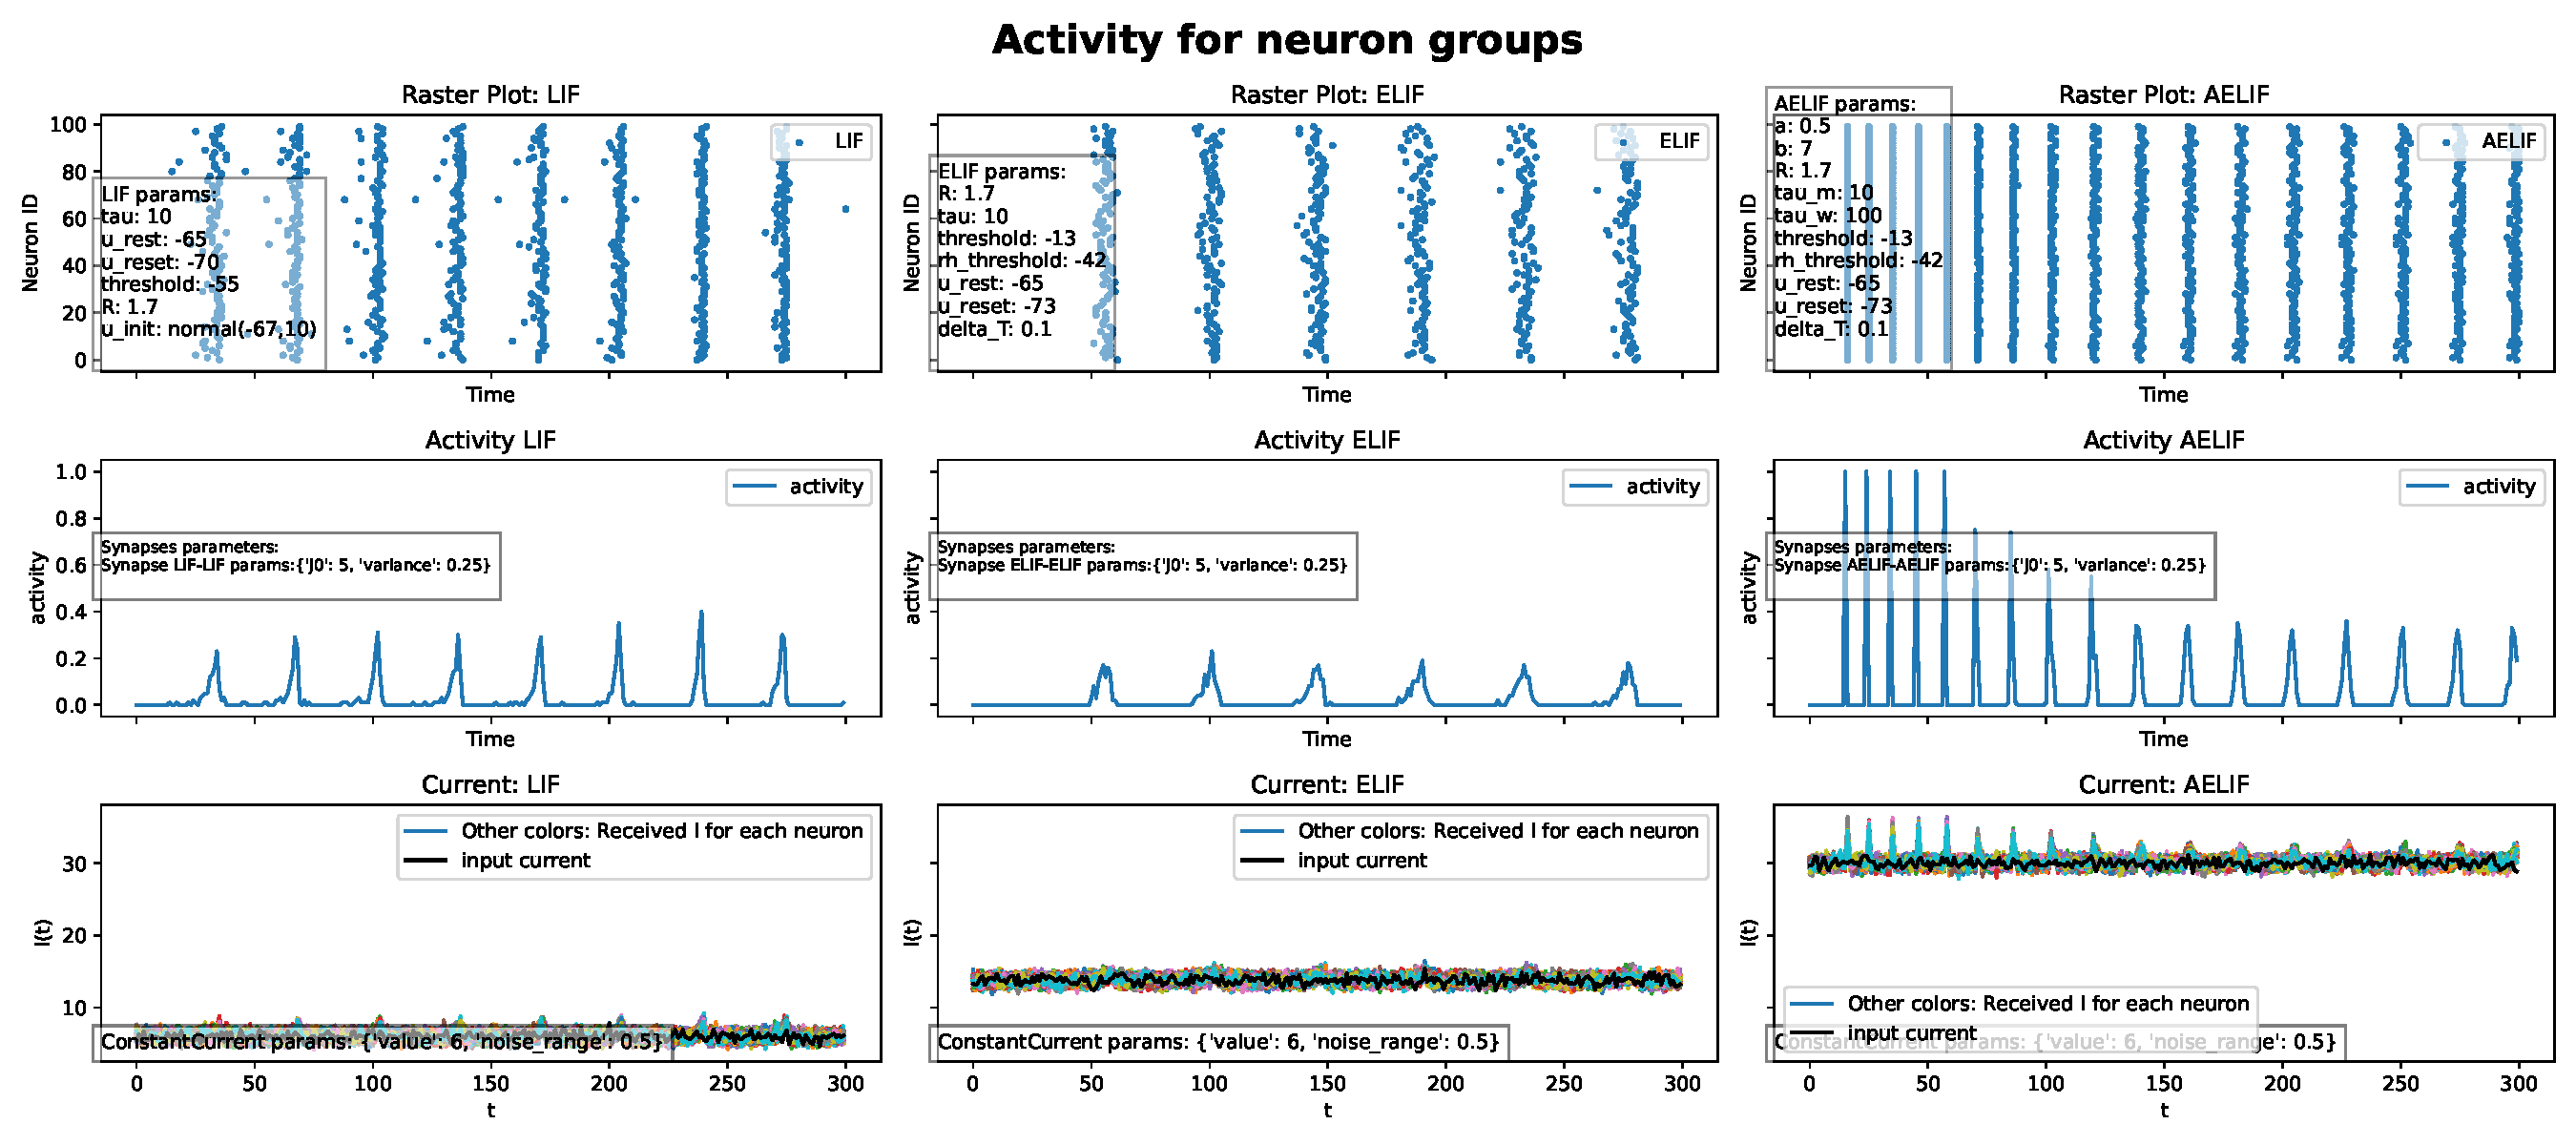
\includegraphics[width=0.9\textwidth]{plots/part2-one-ng-full-synapse-diff-neuron-model.pdf} 
                    \caption{رفتار یک جمعیت نورونی با مدل های نورونی مختلف و جریان تصادفی}
                    \label{fig:part2-one-ng-full-synapse-diff-neuron-model}
                \end{figure}
        \subsubsection{بررسی رفتار دو جمعیت}
            \paragraph*{پارامتر $j_0$}
            حال به بررسی رفتار دو جمعیت که بین آن ها سیناپس قرار دارد می پردازیم. در این بخش   تاثیر دو جمعیت روی یکدیگر را بررسی میکنیم. اولین حالتی که مورد بررسی قرار می دهیم، حالتی است که دو حمعیت تحریکی هستند و فقط به یکدیگر سیناپس دارند و سیناپس داخلی بین نورون های آن ها وجود ندارد.
            در این حالت با نتایجی که تا الآن بدست آورده ایم انتظار داریم که فعالیت دو جمعیت شبیه یک دیگر باشند که شکل
            \ref{fig:part2-two-ng-full-synapse-noise-curr}
            نیز این موضوع را تایید میکند. جریان تصادفی نیز رفتار مشابهی از خود نشان می دهد. 
            (شکل \ref{fig:part2-two-ng-full-synapse-rand-curr})
            \begin{figure}[!ht]
                \centering
                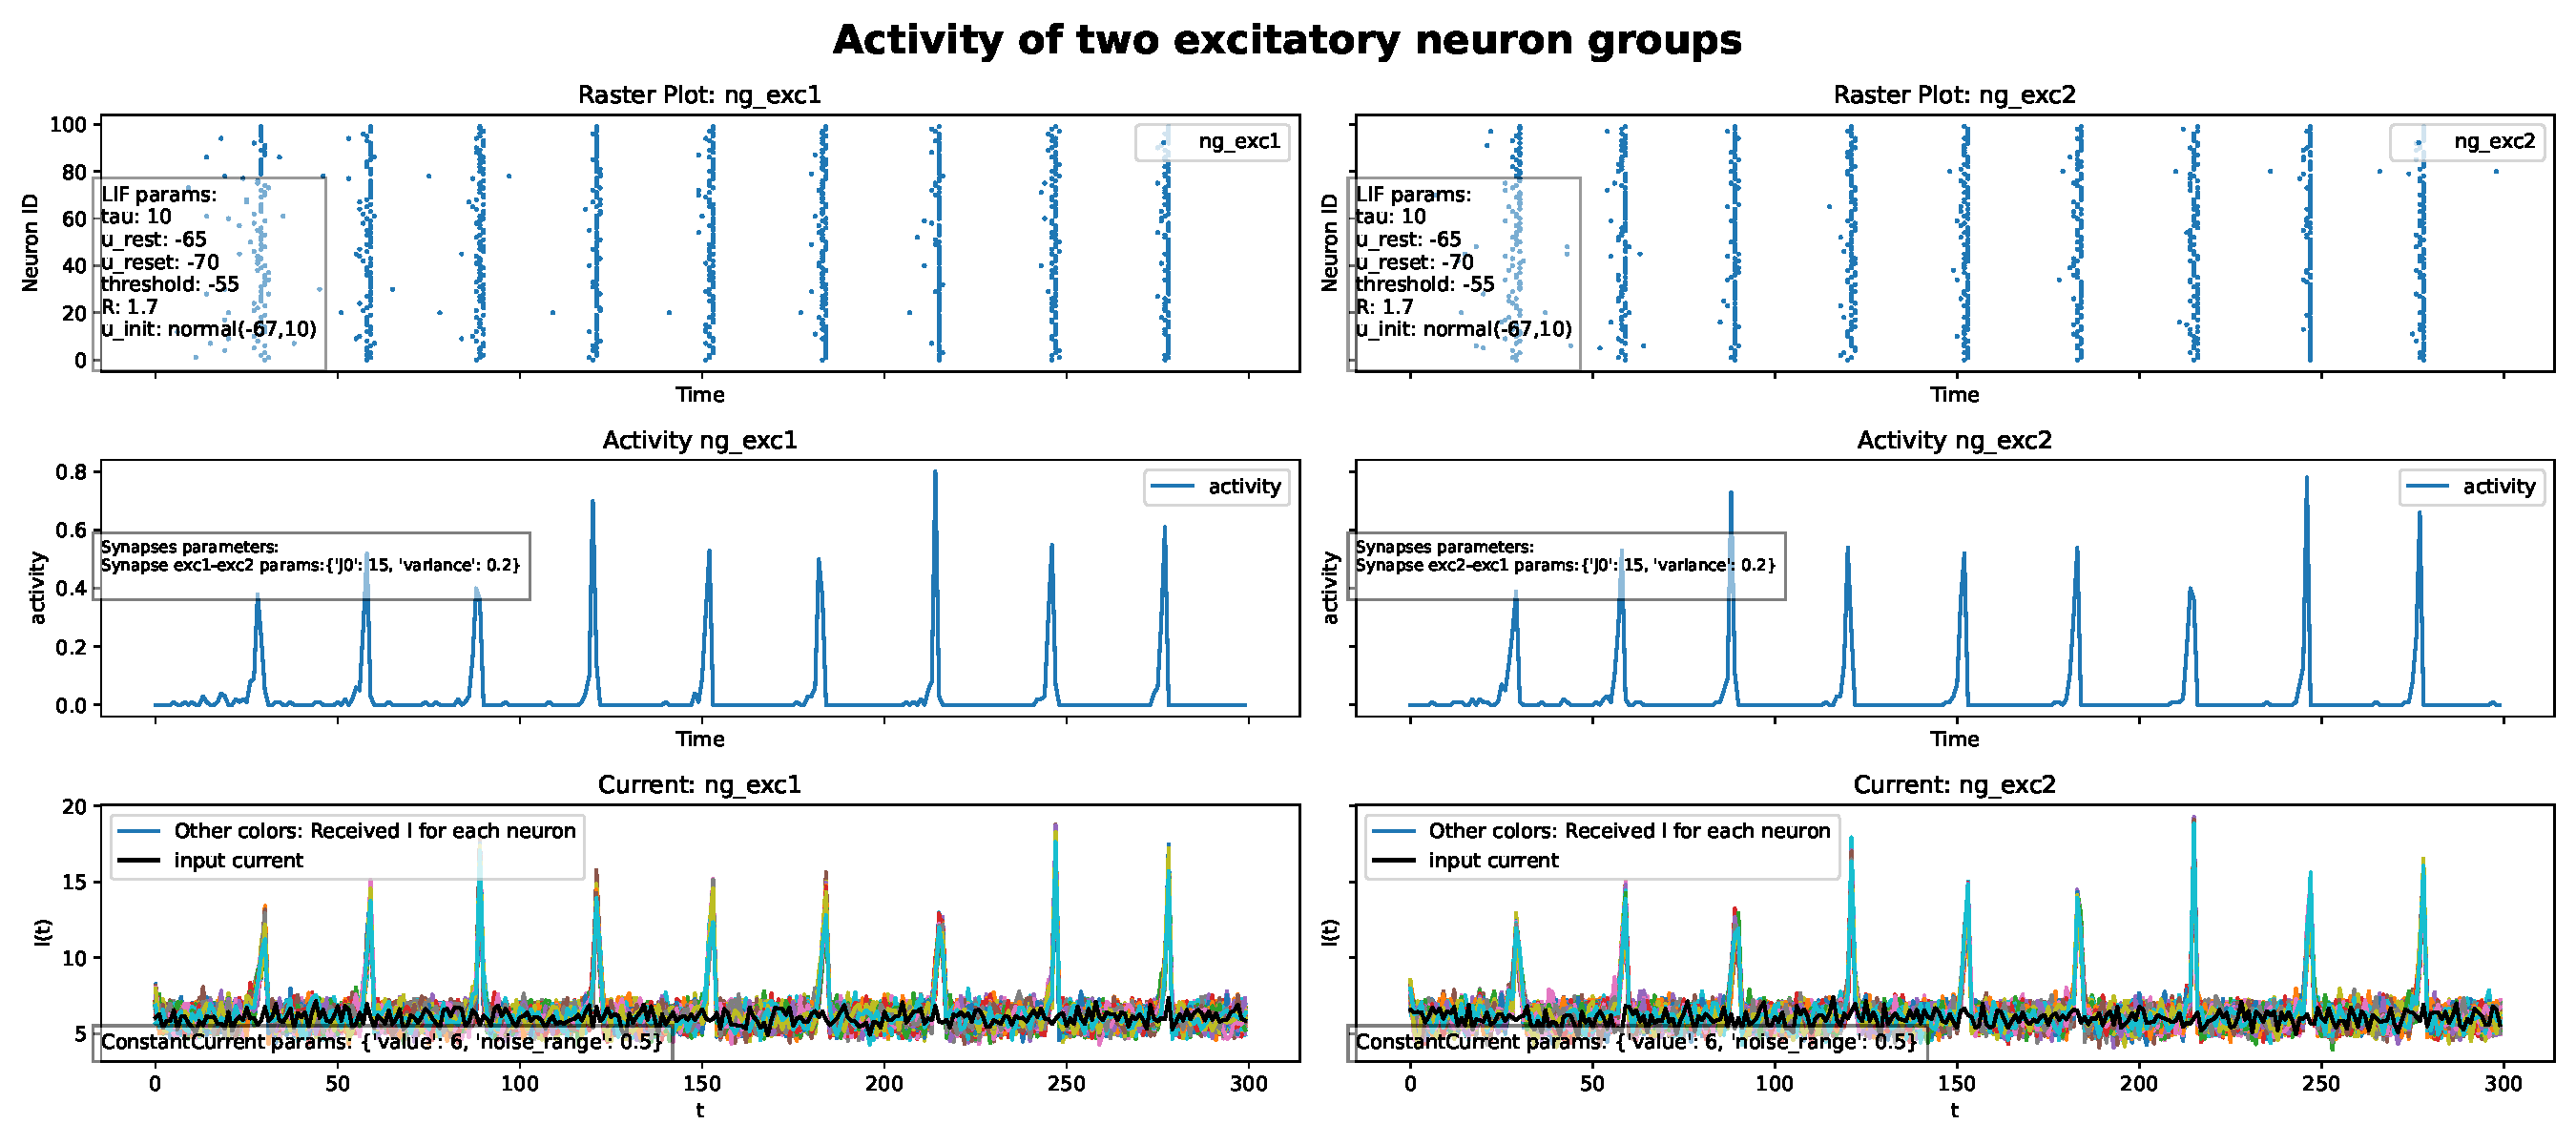
\includegraphics[width=0.9\textwidth]{plots/part2-two-ng-full-synapse-noise-curr.pdf} 
                \caption{رفتار دو جمعیت نورونی با دو سیناپس و جریان ثابت نویزی}
                \label{fig:part2-two-ng-full-synapse-noise-curr}
            \end{figure}
            \begin{figure}[!ht]
                \centering
                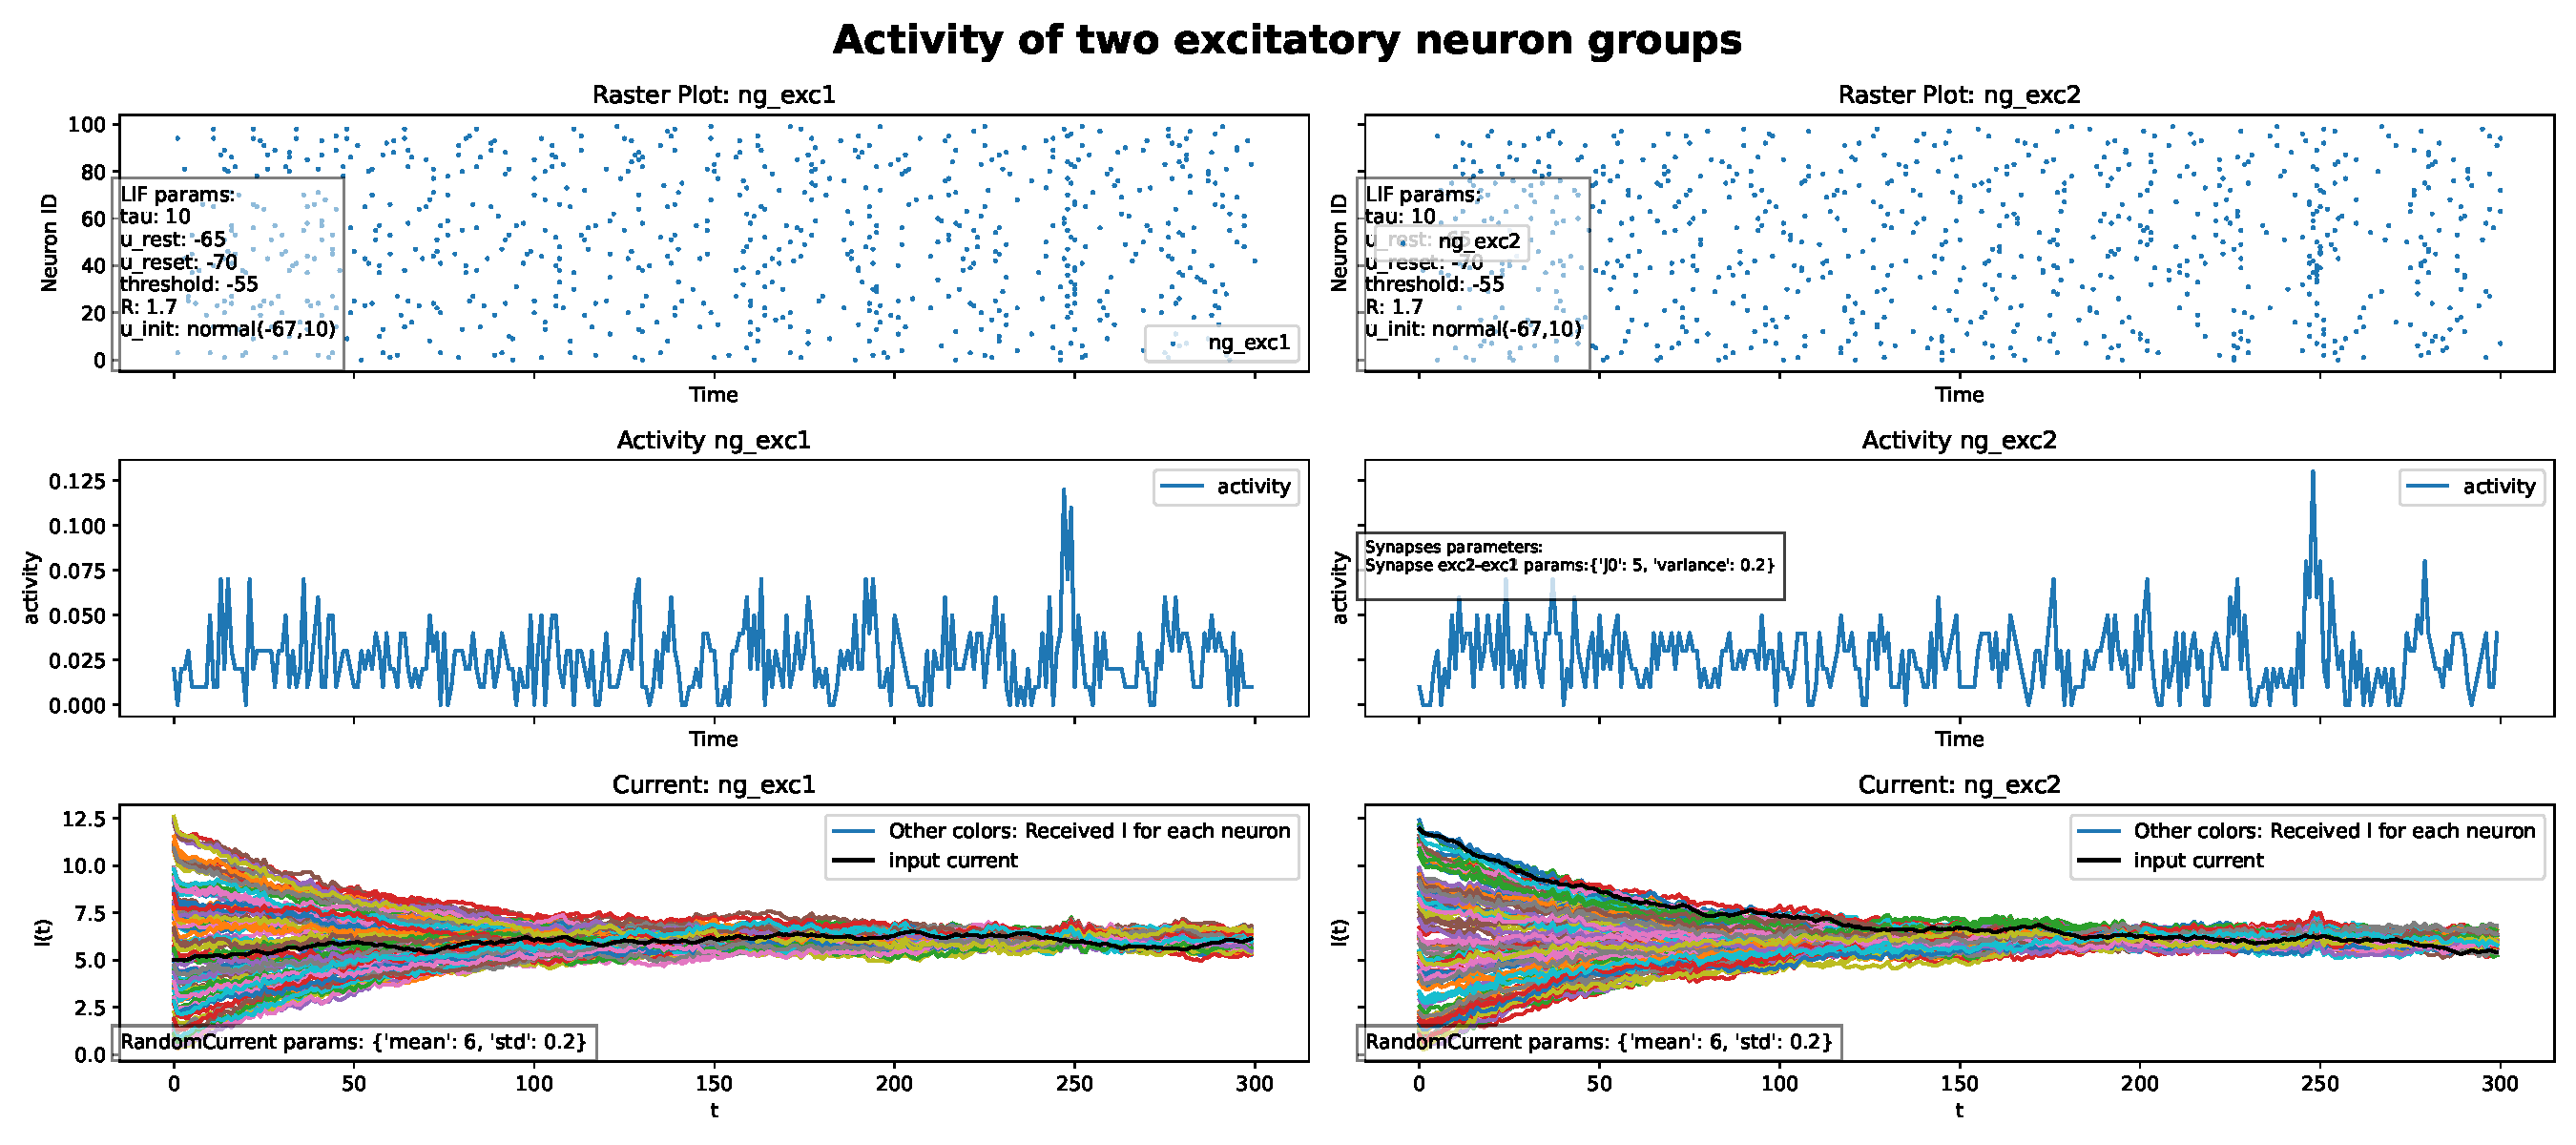
\includegraphics[width=0.9\textwidth]{plots/part2-two-ng-full-synapse-rand-curr.pdf} 
                \caption{رفتار دو جمعیت نورونی با دو سیناپس و جریان تصادفی}
                \label{fig:part2-two-ng-full-synapse-rand-curr}
            \end{figure}

            رفتار جالب دیگری که جریان تصادفی دارد، این است که در ابتدا پراکندگی زمان ضربه زدن نورون ها بسیار زیاد است و الگوی خاصی ندارد، و همچنین فعالیت نورونی کم است، اما همانطور که از نمودار پیداست، این پراکندگی رفته رفته کمتر شده و فعالیت نورونی نیز بیشتر می شود. این اتفاق تحت تاثیر این موضوع است که به دلیل وجود سنیاپس بین دو جمعیت که به صورت رفت و برگشتی است، به گونه ای عمل کرده که هر نورون از تمام نورون های جمعیت دیگر جریان دریافت میکند و درنتیجه جریان دریافتی به نورون زیاد می شود و این جریان زیاد باعث می شود تا پس از مدتی زمان ضربه زدن نورون ها به یکدیگر نزدیک شود.

            حال اگر مقدار 
            $j_0$ 
            را در هر ۲ سیناپس کاهش دهیم چه اتفاقی می افتد؟ شکل 
            \ref{fig:part2-two-ng-full-synapse-low-j-rand-curr}
            به این سوال پاسخ می دهد و بیان می کند که کاهش مقدار 
            $j_0$ 
            باعث می شود تا جریان سیناپسی نتواند آنقدر زیاد شود که در زمان قبلی پراکندگی فعالیت نورون ها را کمتر کند و فعالیت جمعیت به صورت یک نمودار تصادفی با مقدار کم باقی می ماند.(این نکته در بخش های بعدی به کارمان می آید.)
            \begin{figure}[!ht]
                \centering
                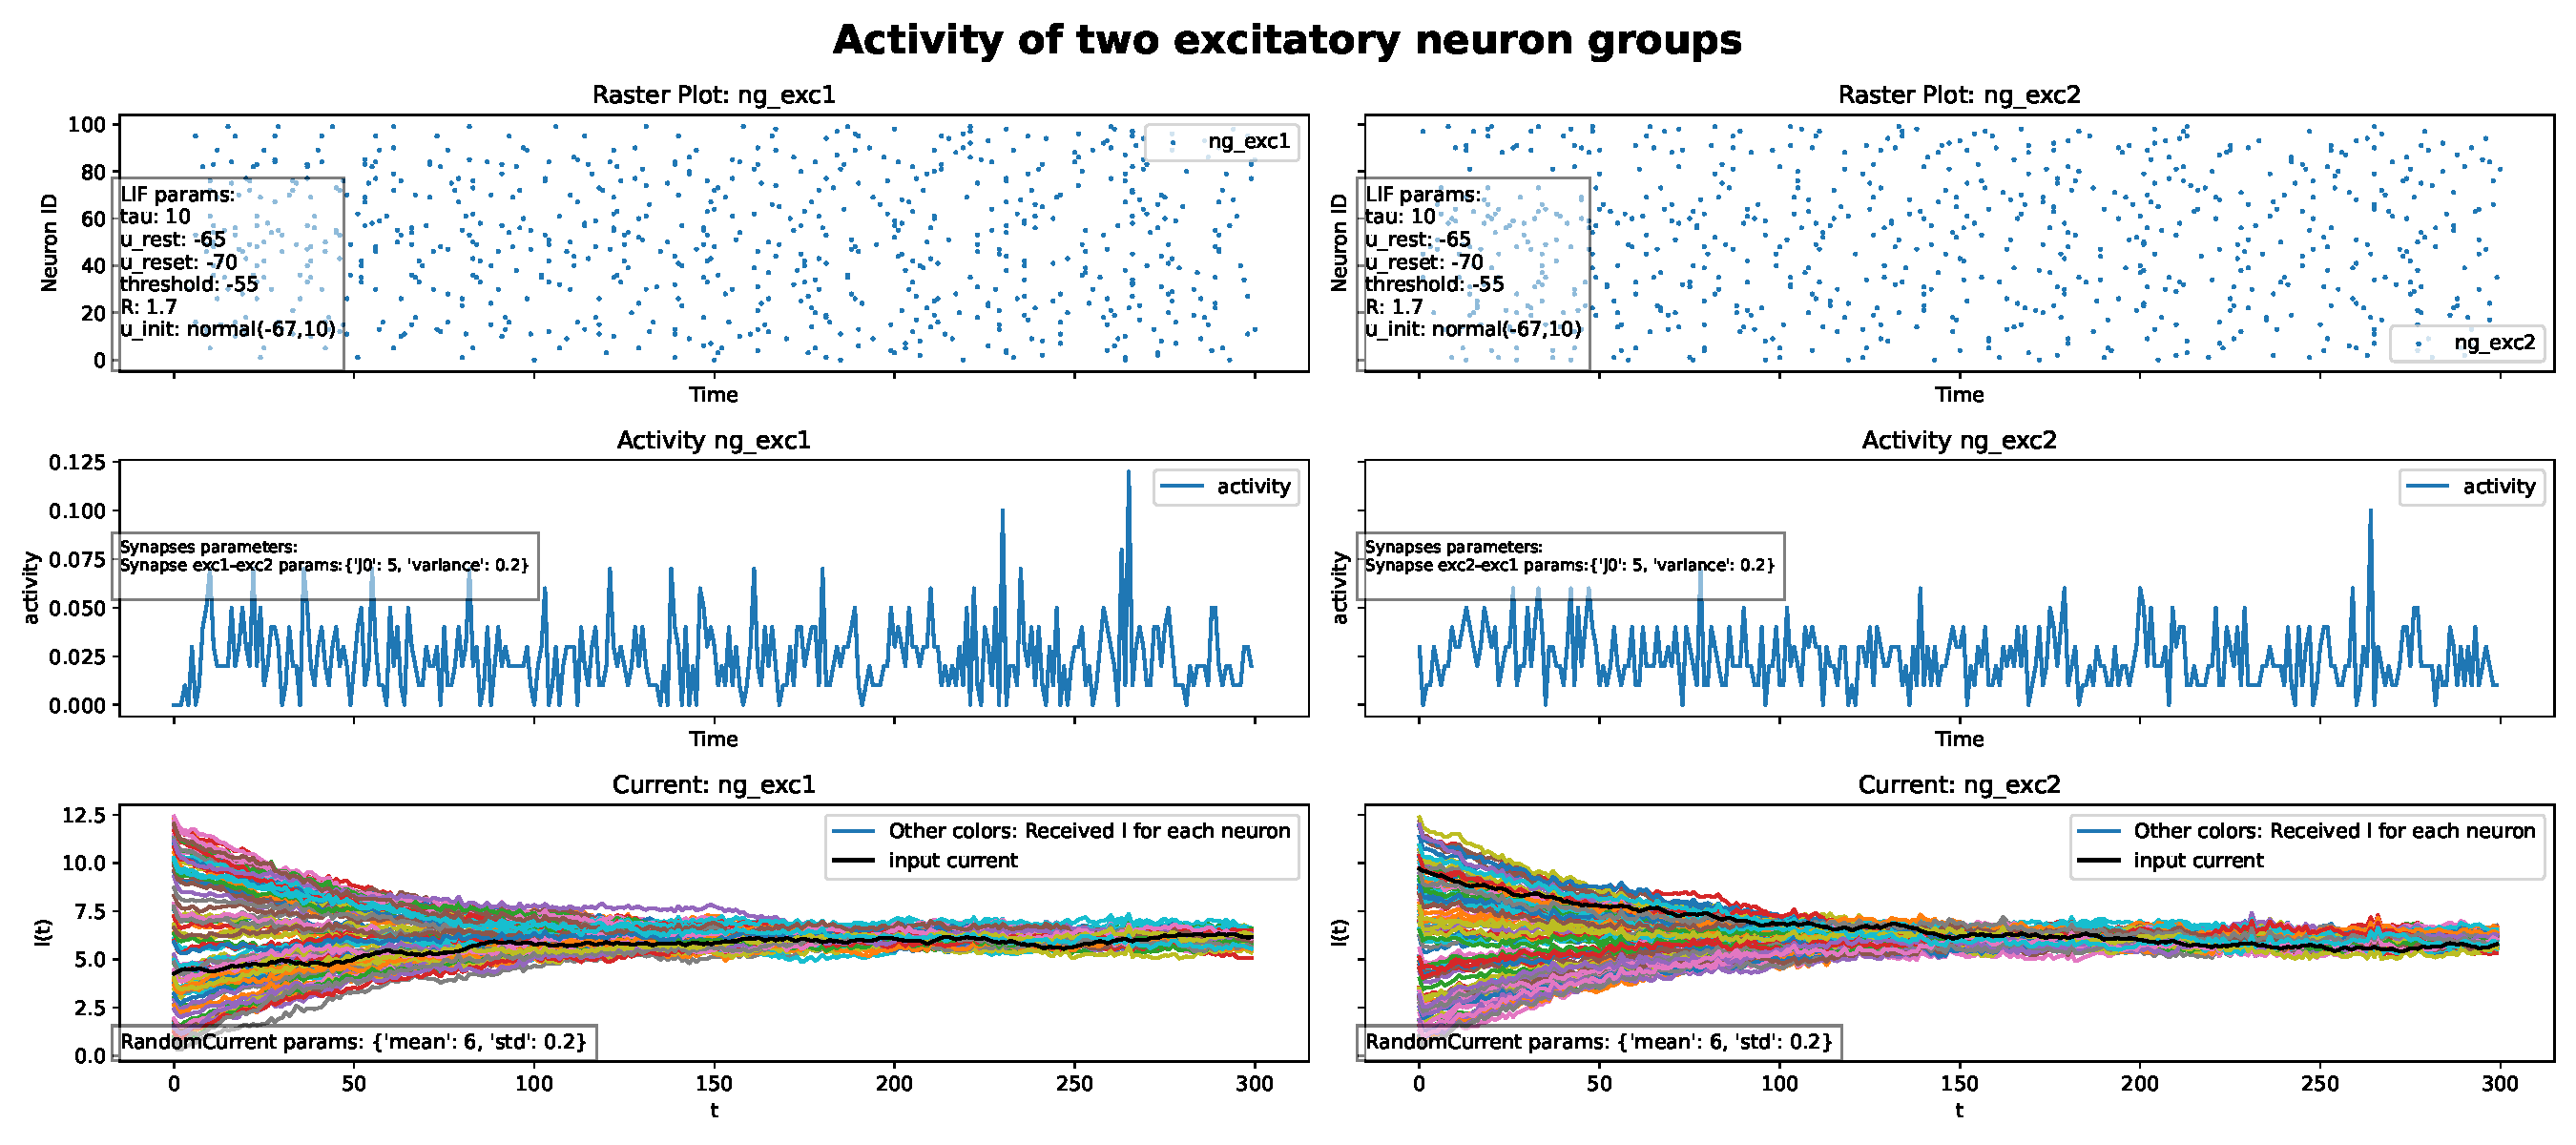
\includegraphics[width=0.9\textwidth]{plots/part2-two-ng-full-synapse-low-j-rand-curr.pdf} 
                \caption{رفتار دو جمعیت نورونی با دو سیناپس و جریان تصادفی و $j_0$ کم}
                \label{fig:part2-two-ng-full-synapse-low-j-rand-curr}
            \end{figure}

            حال مقدار وزن های سیناپس بین جمعیت ۱ به جمعیت ۲ را افزایش میدهیم تا ببینیم با 
            $j_0$
            متفاوت رفتار آن ها چه تغییری میکند. طبق شکل 
            \ref{fig:part2-two-ng-full-synapse-diff-j-rand-curr}
            مشاهده میکنیم که فعالیت هر دو جمعیت بیشتر شده ولی جمعیت ۲ در کل فعالیت بیشتری دارد. مشابه این رفتار را در بخش اول دیدیم، هنگامی که تنها یک سیناپس از جمعیتی به جمعیت دیگر داشتیم و جمعیت پس سیناپسی فعالیت بیشتری داشت. در اینجا نیز گویا همین اتفاق می افتد. بیشتر شدن وزن های سیناپس ۱به۲ باعث می شود که جمعیت ۲ بیشتر ضربه بزند و درنتیجه فعالیت آن بیشتر شود، این بیشتر شدن فعالیت خود باعث می شود که جریان سیناپسی 
            ۲ به ۱
            نیز بیشتر شده و فعالیت جمعیت ۱ نیز بیشتر شود. اما در کل از آنجا که وزن های سیناپسی جمعیت ۱ به ۲ بیشتر است، فعالیت جمعیت ۲ بیشتر از ۱ میماند.
            \begin{figure}[!ht]
                \centering
                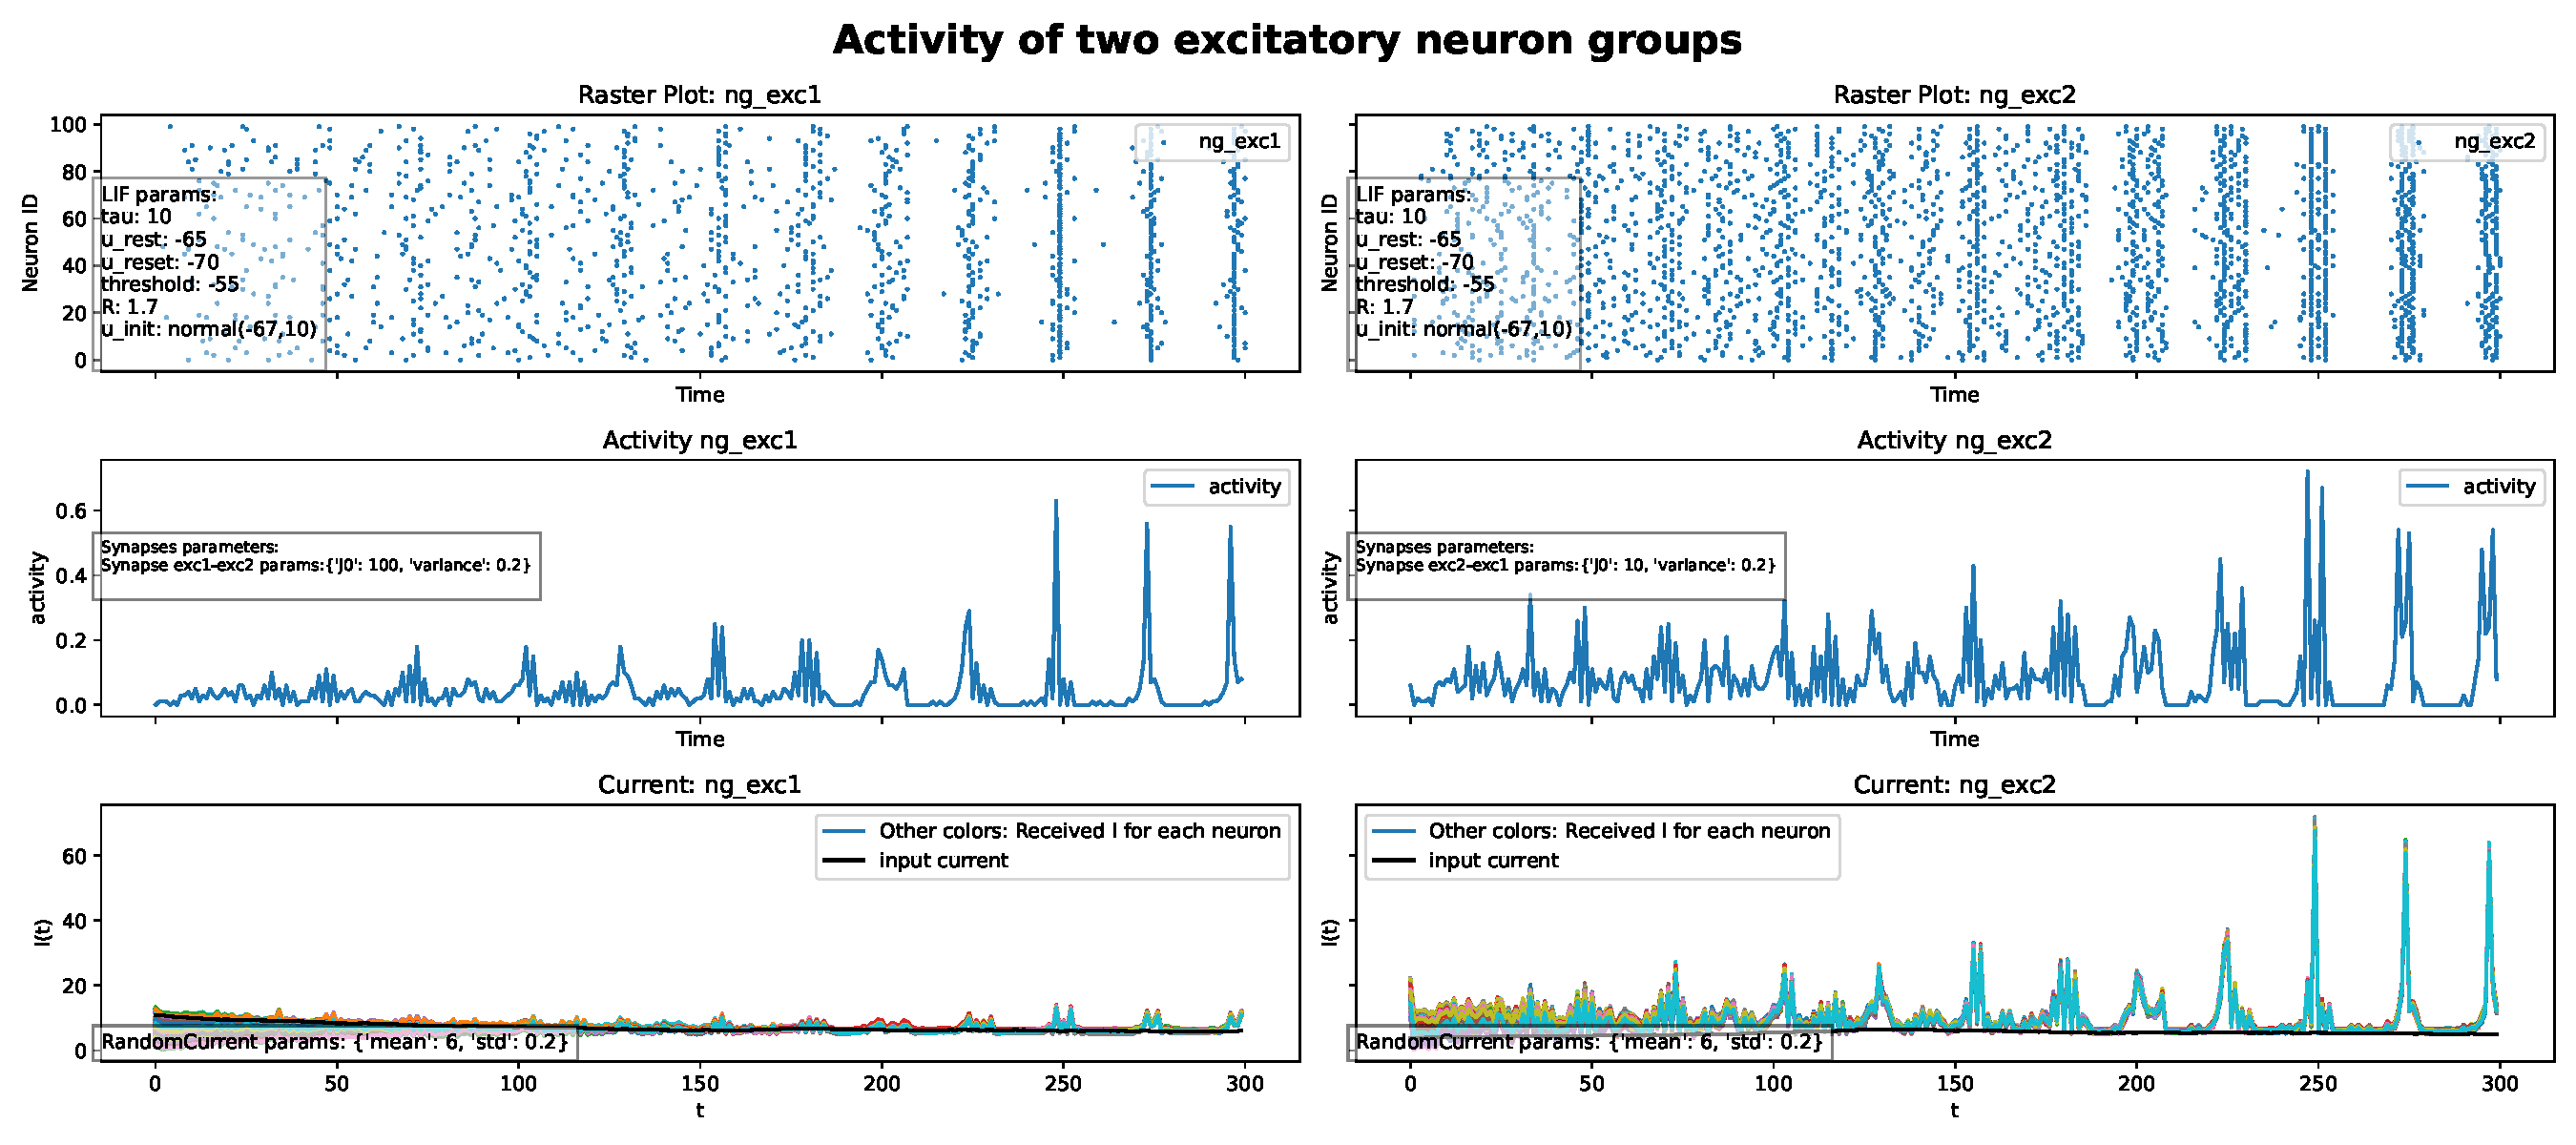
\includegraphics[width=0.9\textwidth]{plots/part2-two-ng-full-synapse-diff-j-rand-curr.pdf} 
                \caption{رفتار دو جمعیت نورونی با دو سیناپس و جریان تصادفی و $j_0$ متفاوت}
                \label{fig:part2-two-ng-full-synapse-diff-j-rand-curr}
            \end{figure}
        \paragraph*{پارامتر واریانس}
            حال با وزن های برابر با شکل 
            \ref{fig:part2-two-ng-full-synapse-noise-curr}
            مقادیر واریانس را افزایش داده و آن را تحلیل میکنیم.
            همانطور که در شکل 
            \ref{fig:part2-two-ng-full-synapse-high-variance-noise-curr}
            مشاهده می شود، افزایش واریانس به علت مشابهی که قبل تر نتیجه گرفته شد، تغییر چندانی در رفتار نورون با جریان های متفاوت ایجاد نمی کند.
            \begin{figure}[!ht]
                \centering
                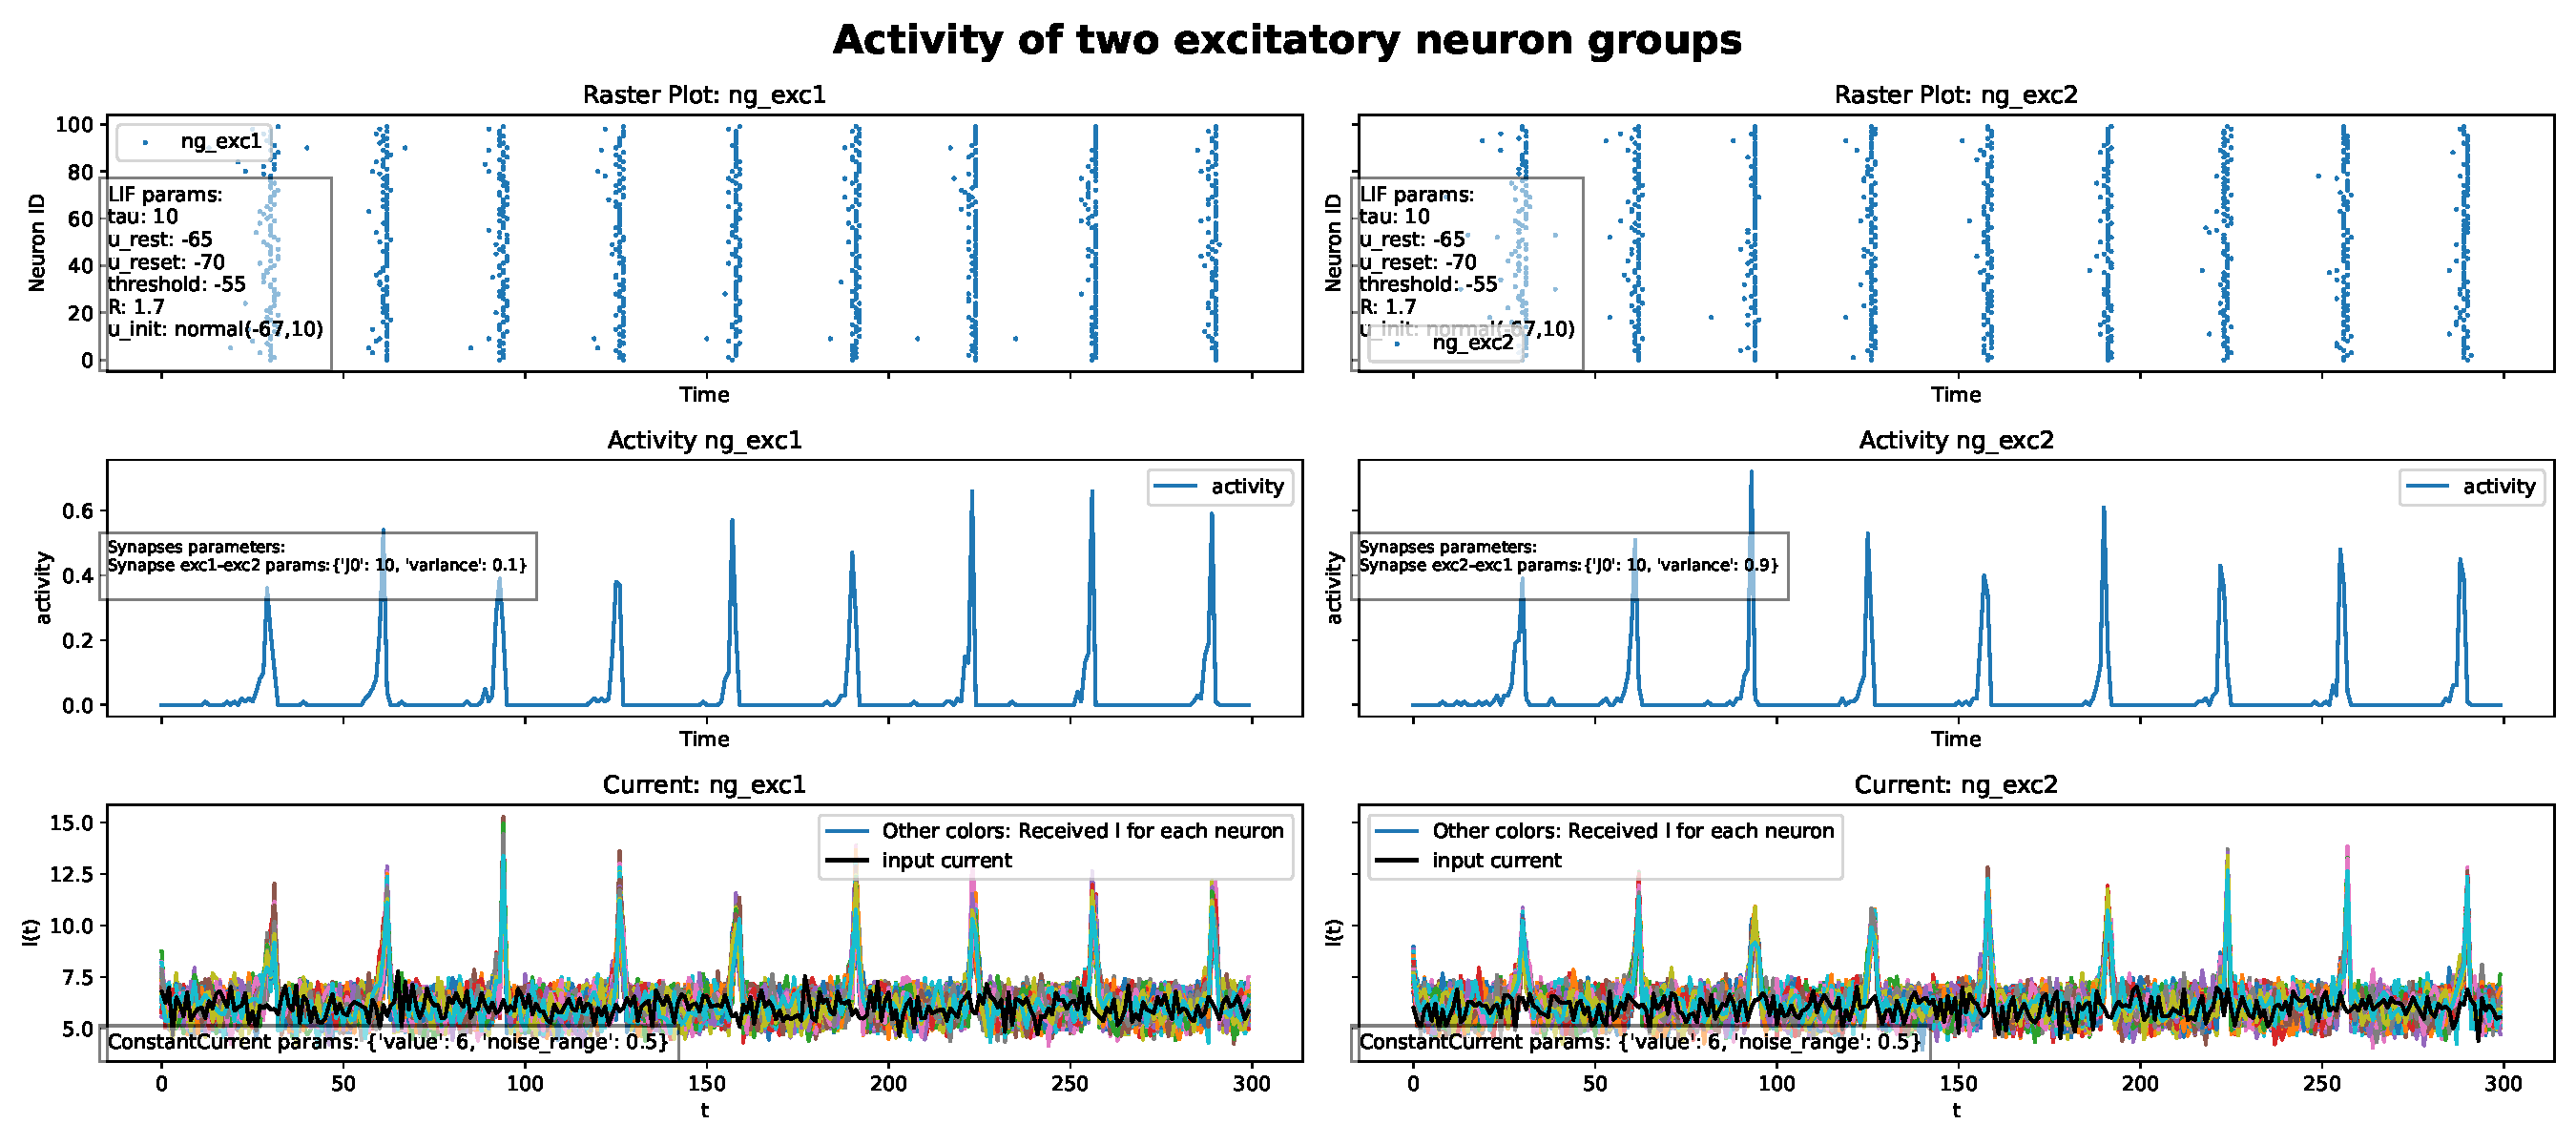
\includegraphics[width=0.9\textwidth]{plots/part2-two-ng-full-synapse-diff-variance-noise-curr.pdf} 
                \caption{رفتار دو جمعیت نورونی با دو سیناپس و جریان نویزی و واریانس زیاد}
                \label{fig:part2-two-ng-full-synapse-high-variance-noise-curr}
            \end{figure}

            مجددا مقدار واریانس ها را متفاوت در نظر میگریم و طبق شکل
            \ref{fig:part2-two-ng-full-synapse-diff-variance-rand-curr}
            مشاهده می شود که با واریانس متفاوت نیز تغییری در رفتار نورون ها اتفاق نمی افتد. طبعا نتیجه برای جریان تصادفی نیز به همین صورت است.
            \begin{figure}[!ht]
                \centering
                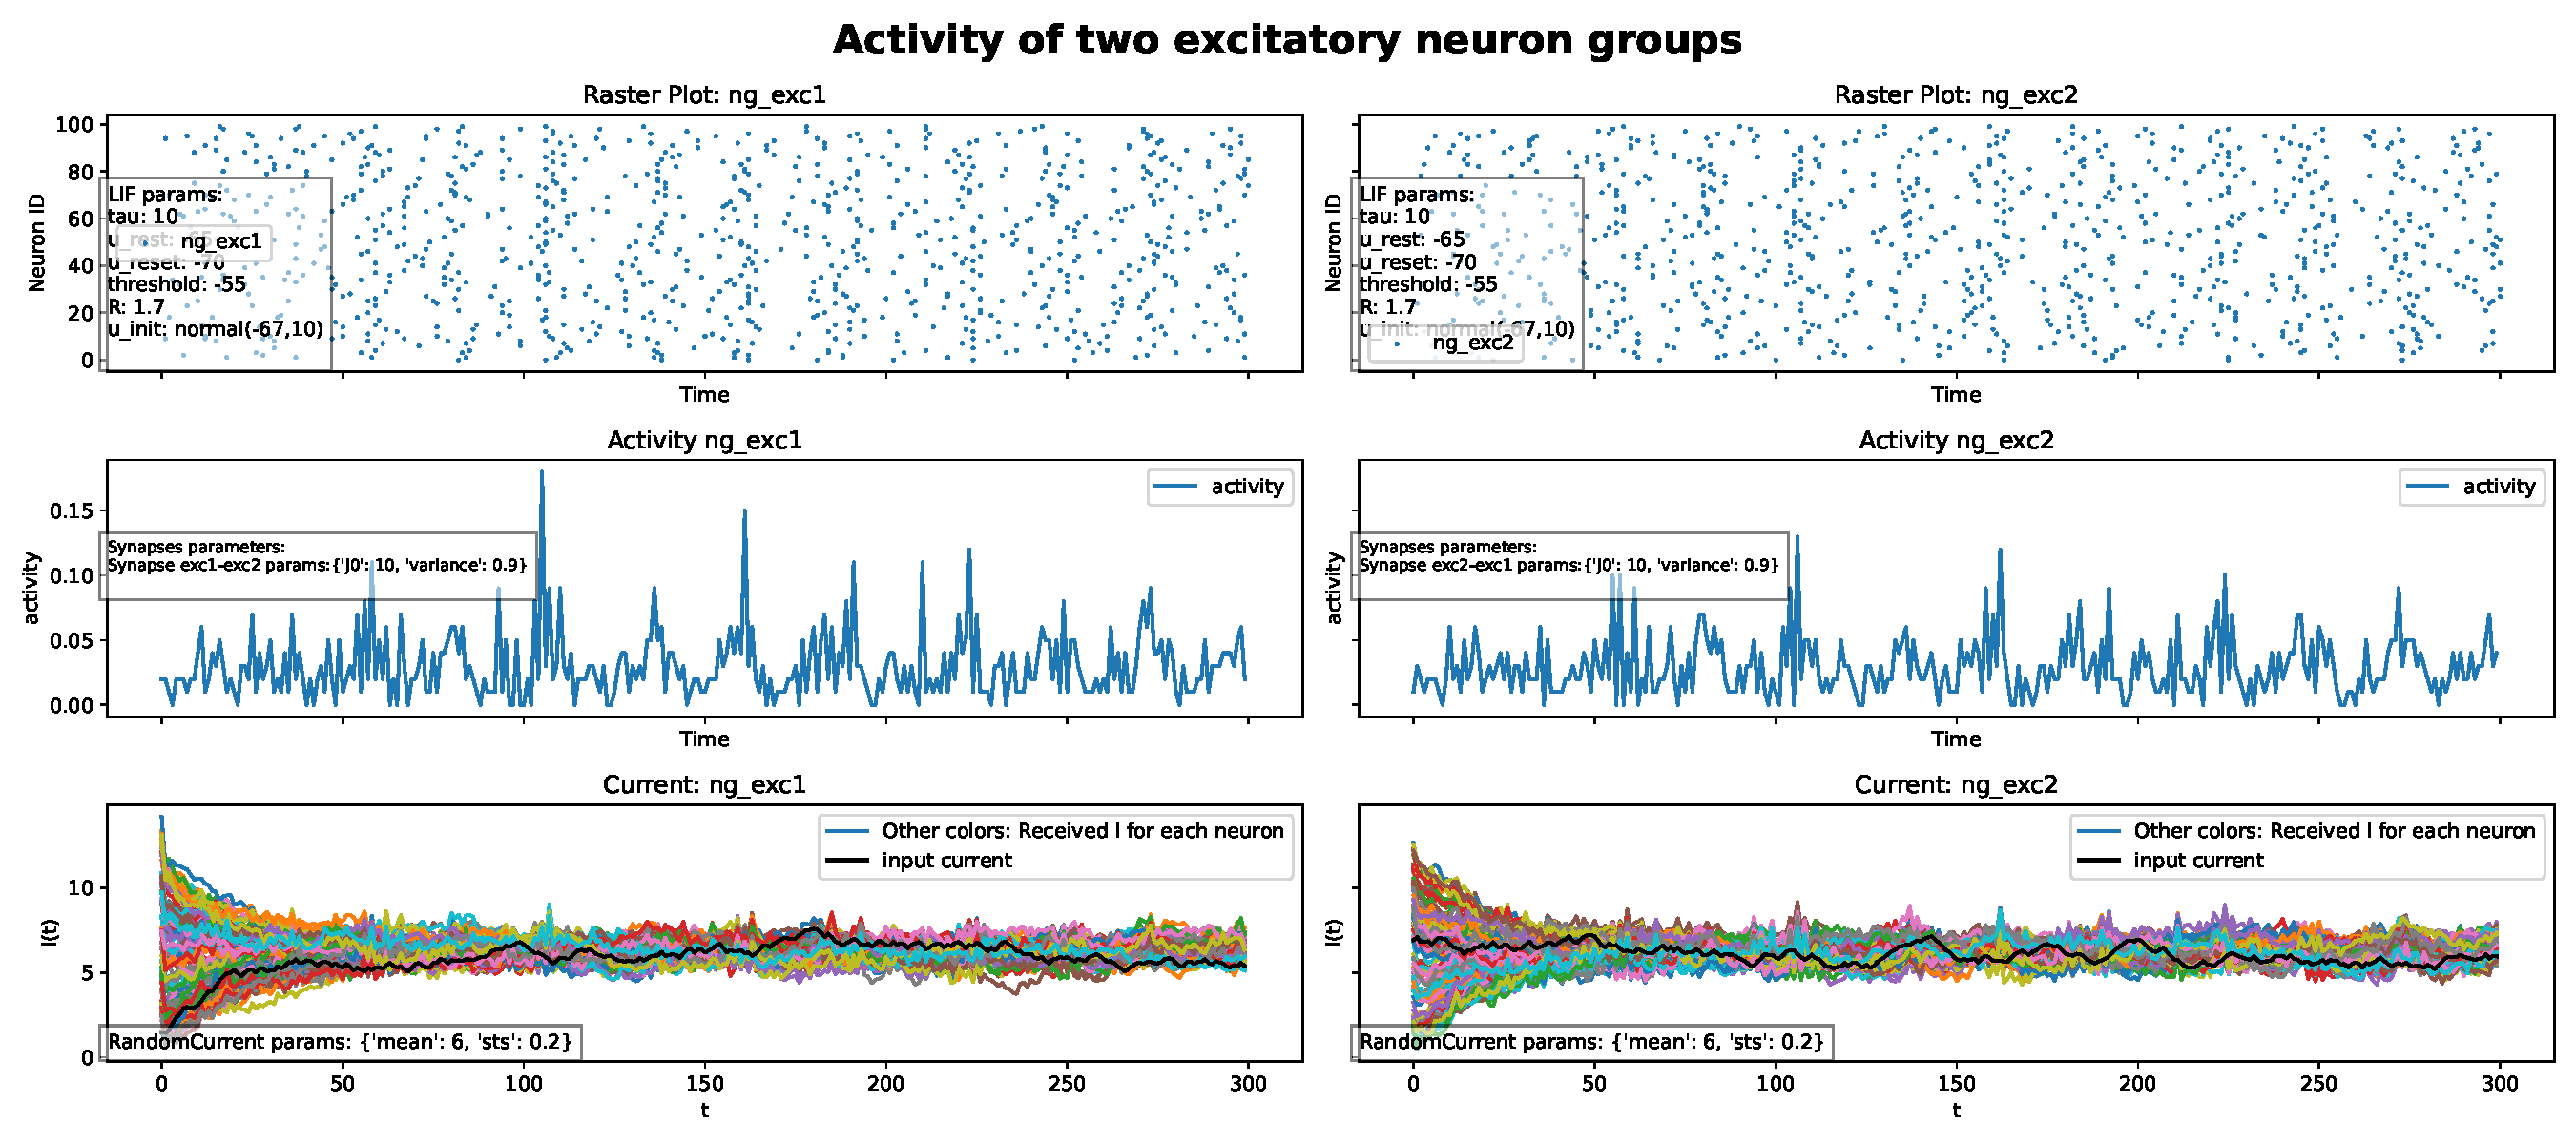
\includegraphics[width=0.9\textwidth]{plots/part2-two-ng-full-synapse-diff-variance-rand-curr.pdf} 
                \caption{رفتار دو جمعیت نورونی با دو سیناپس و جریان نویزی و واریانس متفاوت}
                \label{fig:part2-two-ng-full-synapse-diff-variance-rand-curr}
            \end{figure}
            همانطور که پیشتر گفته شد، اگر بخواهیم واریانس را به گونه ای تغییر دهیم که تاثیر قابل نمایشی داشته باشد، باید مقدار آن را زیادتر، مثلا ۱۰۰ بگیریم. مطابق شکل 
            \ref{fig:part2-two-ng-full-synapse-very-high-variance-noise-curr}
            تاثیر این مقدار نمایان است. این به این دلیل است که با خیلی زیاد شدن واریانس، بسیاری از وزن ها نیز آنقدر زیاد می شوند که تاثیر مجموع آن ها روی نورون های پس سیناپسی مشهود می شود.
            \begin{figure}[!ht]
                \centering
                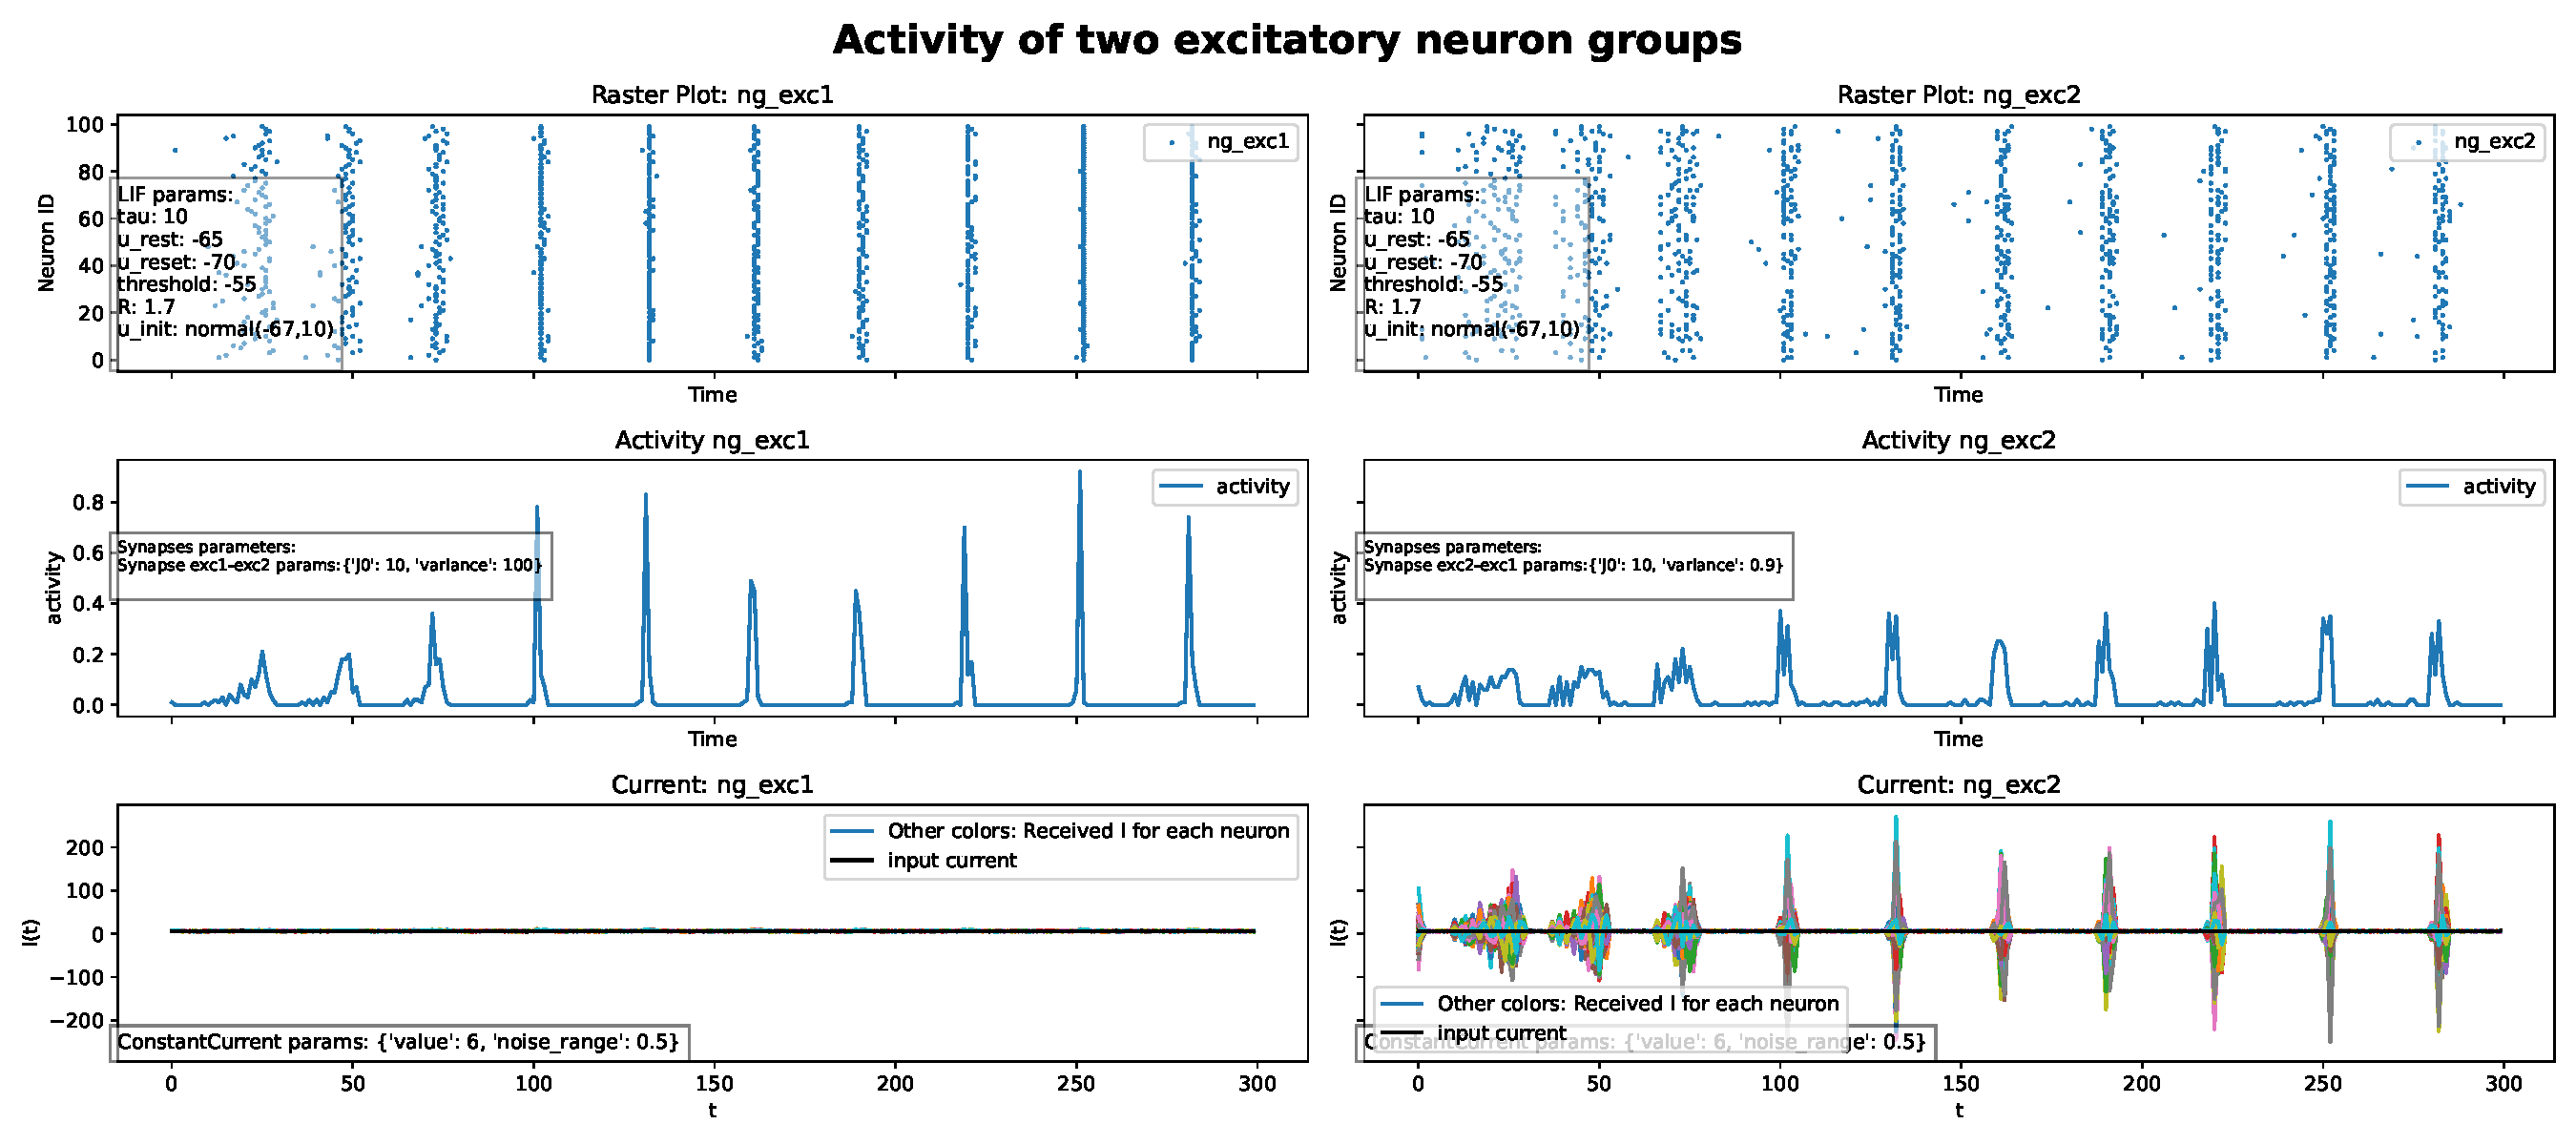
\includegraphics[width=0.9\textwidth]{plots/part2-two-ng-full-synapse-very-high-variance-noise-curr.pdf} 
                \caption{رفتار دو جمعیت نورونی با دو سیناپس و جریان نویزی و واریانس بسیار زیاد}
                \label{fig:part2-two-ng-full-synapse-very-high-variance-noise-curr}
            \end{figure}
            
            \paragraph*{تاثیر اندازه جمعیت}
            از آنجا که تنها دو جمعیت نورونی داریم، زیاد کردن هر دو جمعیت تاثیری مشابه تک جمعیت خواهد داشت، در نتیجه فقط حالتی را که یک جمعیت بزرگتر از دیگری است را آزمایش میکنیم. در این حالت نیز مشابه حالت های قبل میبینیم که فعالیت هر دو جمعیت پس از مدتی بیشتر می شود. هر چند میزان رشد جمعیت بزرگتر اندکی از جمعیت کوچکتر بیشتر است.
            (شکل \ref{fig:part2-two-ng-full-synapse-diff-size-noise-curr})
            \begin{figure}[!ht]
                \centering
                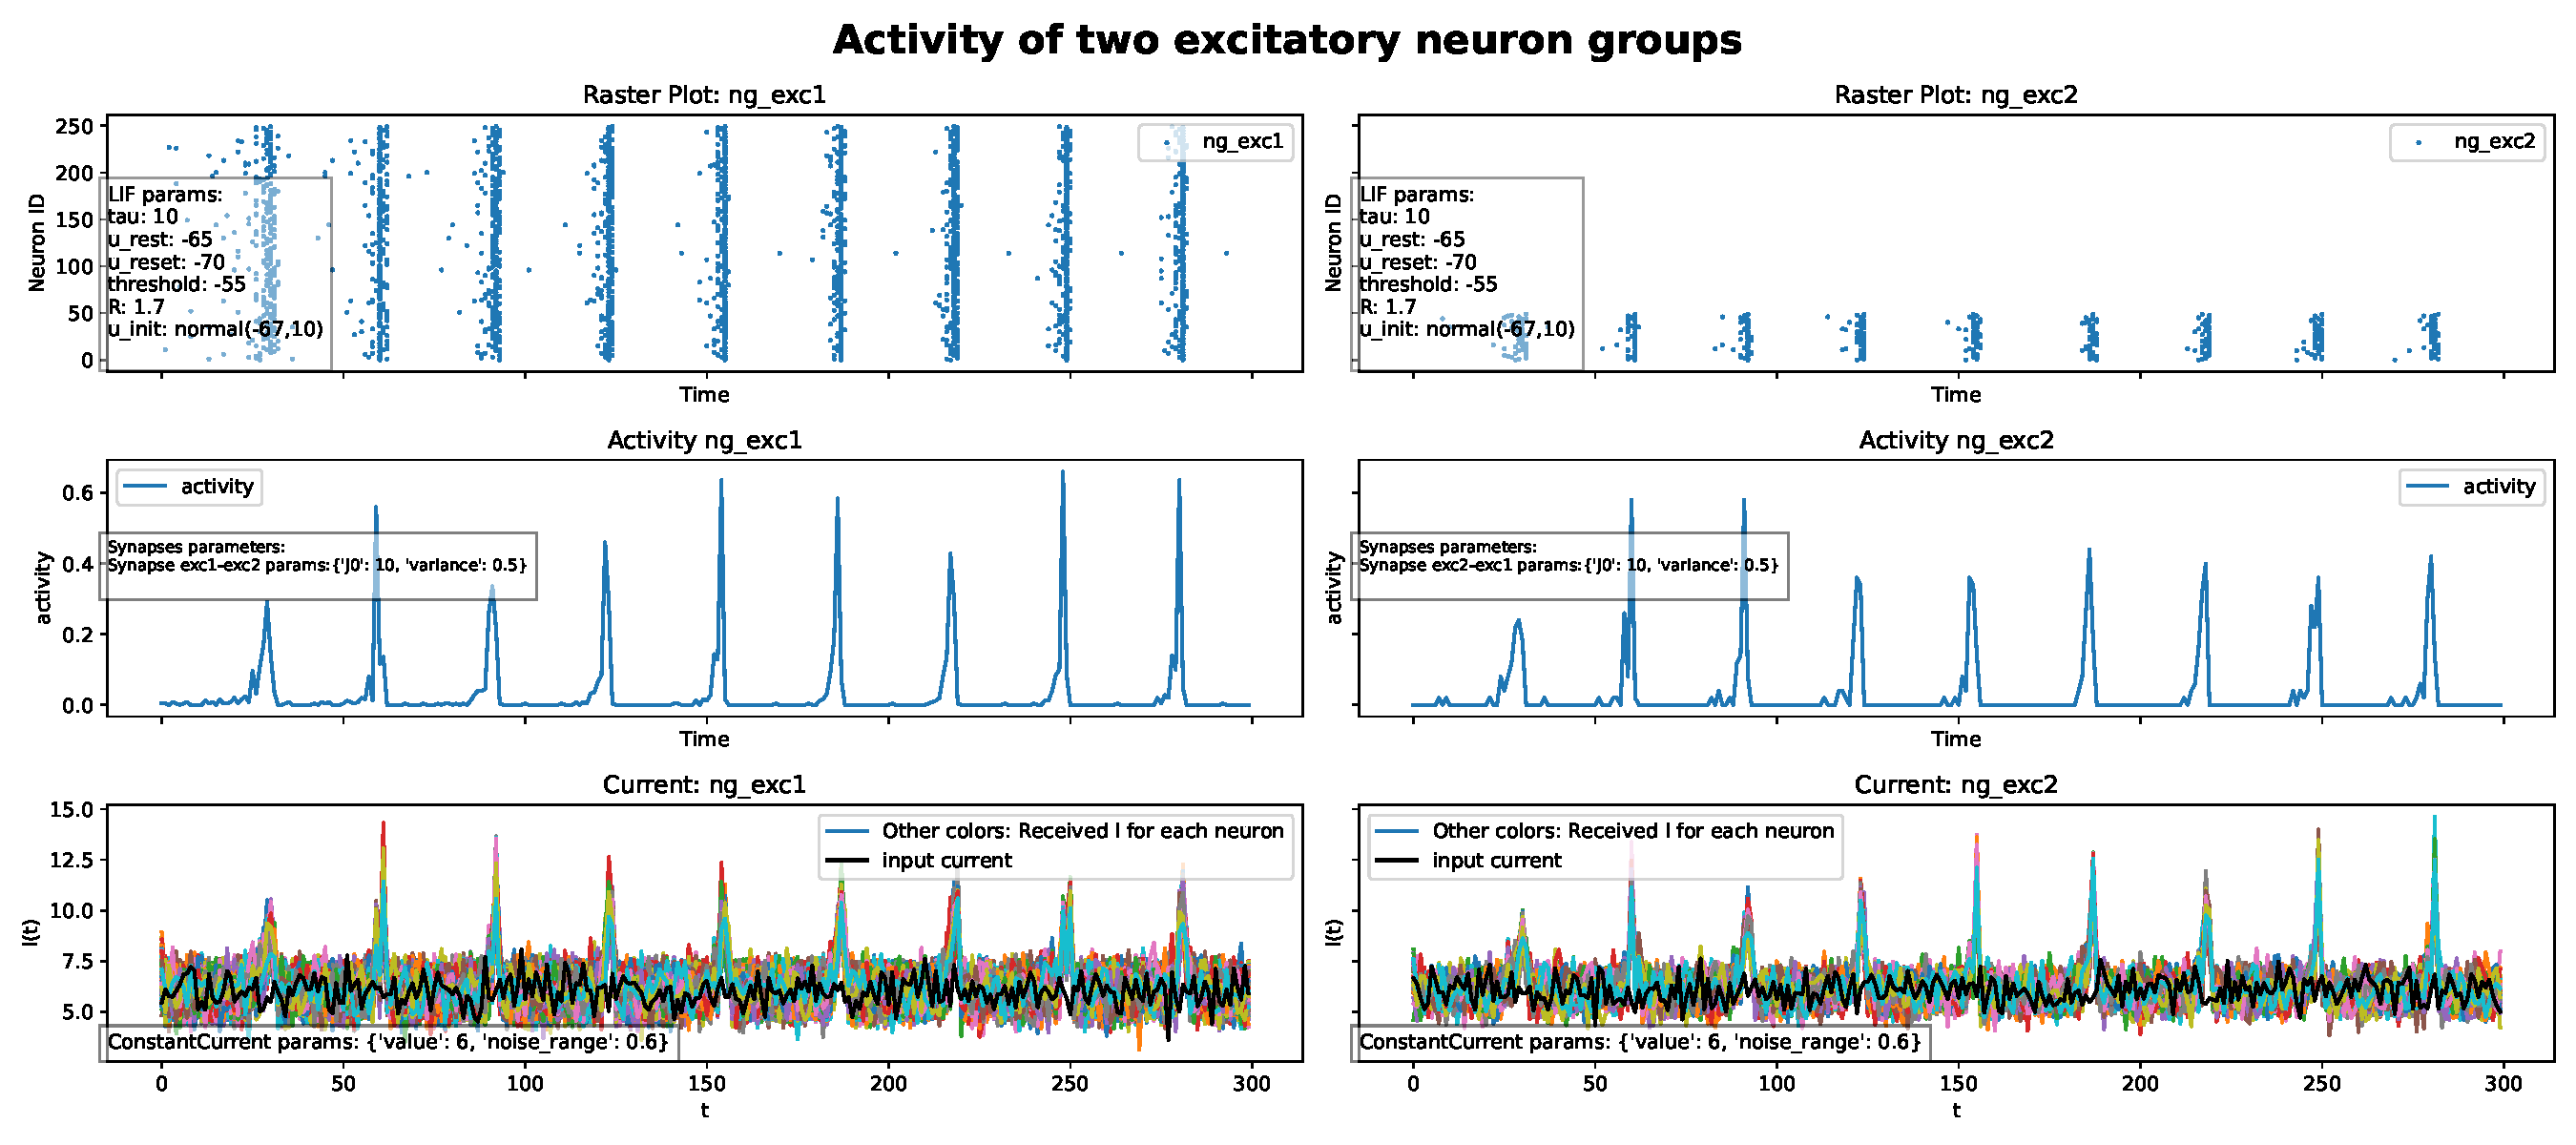
\includegraphics[width=0.9\textwidth]{plots/part2-two-ng-full-synapse-diff-size-noise-curr.pdf} 
                \caption{رفتار دو جمعیت نورونی با دو سیناپس و جریان نویزی و جمعیت متفاوت}
                \label{fig:part2-two-ng-full-synapse-diff-size-noise-curr}
            \end{figure}


    \subsection{الگوی ارتباط تصادفی با احتمال جفت شدن ثابت}
        در این قسمت به بررسی رفتار الگوی ارتباط تصادفی با احتمال جفت شدن ثابت می پردازیم. 

        از نظر تجربی، احتمال 
        $p$
        که یک نورون در داخل یک ستون قشر مغز، یک اتصال عملکردی به نورون دیگری در همان ستون برقرار کند، در محدوده 10 درصد است، هرچند این مقدار در بین لایه‌ها متفاوت است.

        در شبیه‌سازی‌ها، می‌توانیم یک احتمال اتصال 
        $p$ 
        را رفع کنیم و اتصالات را به‌طور تصادفی با احتمال 
        $p$ 
        از بین تمام اتصالات 
        $N^2$ 
        ممکن انتخاب کنیم. در این مورد، تعداد اتصال های ورودی پیش سیناپسی 
        $C_j$
        به یک نورون پس سیناپسی 
        $j$
        دارای مقدار میانگین 
        $\langle C_j = pN\rangle$
        است، اما بین یک نورون و نورون بعدی با واریانس 
        $p(1-p)N$ 
        در نوسان است.

        تا اینجای کار تاثیر بسیاری از پارامتر هایی که بررسی کردم شبیه تاثیر پارامتر های مشابه این الگو است. از این رو در این بخش تمرکزمان را روی پارامتر هایی میگذاریم که تاثیر متفاوت تری نسبت به حالت قبل دارند. در اینجا نیز مدل نورونی را مانند مدل های قبل درنظر میگیریم.
        \subsubsection*{بررسی رفتار یک جمعیت}
            برای شروع کار، بیایید رفتار یک جمعیت را با جریان ثابت، نویزی و تصادفی بررسی کنیم. همانطور که از شکل 
            \ref{fig:part2-one-ng-prob-synapse-diff-curr}
            بر می‌آید، رفتار نورون همانند الگوی ارتباط قبلی بوده و پس از مدتی، پراکندگی زمان ضربه زدن نورون ها کمتر شده و فعالیت رفته رفته بیشتر می شود و این بیشتر شدن به ترتیب نمودار ها از سمت چپ به راست سرعت کمتری دارد. دلیل این امر نیز مشابه الگو های قبل، زیاد شدن جریان سیناپسی است.
            \begin{figure}[!ht]
                \centering
                \includegraphics[width=0.9\textwidth]{plots/part2-one-ng-prob-synapse-diff-curr.pdf} 
                \caption{رفتار تک جمعیت های نورونی با سیناپس داخلی و جریان ثابت، نویزی و تصادفی}
                \label{fig:part2-one-ng-prob-synapse-diff-curr}
            \end{figure}
            
            حال به سراغ آزمایش پارامترها میرویم. پارامتر 
            $j_0$ 
            تاثیری مشابه الگوی قبلی دارد و خیلی روی آن تمرکز نمیکنیم
            \paragraph*{پارامتر $j_0$}
                همانطور که در شکل
                \ref{fig:part2-one-ng-prob-synapse-diff-j-rand-curr}
                مشاهده می شود، افزایش مقدار 
                $j_0$ 
                باعث کاهش پراکندگی زمان ضربه زدن نورون ها و افزایش فعالیت جمعیت می شود. همانطور که از شکل نیز بر می آید، دلیل این امر مانند الگوی گذشته، افزایش جریان سیناپسی و درنتیجه افزایش فعالیت جمعیت است.
                \begin{figure}[!ht]
                    \centering
                    \includegraphics[width=0.9\textwidth]{plots/part2-one-ng-prob-synapse-diff-j-rand-curr.pdf} 
                    \caption{رفتار تک جمعیت های نورونی با سیناپس داخلی و جریان تصادفی $j_0$ متفاوت}
                    \label{fig:part2-one-ng-prob-synapse-diff-j-rand-curr}
                \end{figure}

            
            \paragraph*{پارامتر واریانس}
                برای درک بهتر تاثیر این پارامتر، ابتدا یک جریان تصادفی ولی یکسان برای همه نورون ها به جمعیت میدهیم.
                در این الگو طبق شکل 
                \ref{fig:part2-one-ng-prob-synapse-diff-variance-same-rand-curr}
                ملاحظه میکنیم که تغییر در واریانس میتواند مقدار کمی رفتار جمعیت را تغییر دهد. بدین صورت که با افزایش واریانس از 
                $0.2$ 
                تا
                $0.6$ 
                وزن های اولیه، باعث می شود فعالیت جمعیت کاهش یابد. اگر آزمایش را با همین پارامتر ها ولی با جریان تصادفی غیر یکسان اجرا کنیم، میبینیم که تاثیر واریانس کمرنگ تر می شود.
                (شکل \ref{fig:part2-one-ng-prob-synapse-diff-variance-rand-curr})
                \begin{figure}[!ht]
                    \centering
                    \includegraphics[width=0.9\textwidth]{plots/part2-one-ng-prob-synapse-diff-variance-same-rand-curr.pdf} 
                    \caption{رفتار تک جمعیت های نورونی با سیناپس داخلی و جریان تصادفی یکسان و واریانس متفاوت}
                    \label{fig:part2-one-ng-prob-synapse-diff-variance-same-rand-curr}
                \end{figure}
                \begin{figure}[!ht]
                    \centering
                    \includegraphics[width=0.9\textwidth]{plots/part2-one-ng-prob-synapse-diff-variance-rand-curr.pdf} 
                    \caption{رفتار تک جمعیت های نورونی با سیناپس داخلی و جریان تصادفی و واریانس متفاوت}
                    \label{fig:part2-one-ng-prob-synapse-diff-variance-rand-curr}
                \end{figure}
            
            \paragraph*{پارامتر $p$}
                حال نوبت به پارامتر جدید این الگو می رسد. این پارامتر  بیان می دارد که هر نورون با چه احتمالی با نورون های دیگر در ارتباط باشد. در آزمایش اول نیز همانند قبل، ابتدا جمعیت را با جریان تصادفی یکسان آزمایش میکنیم. طبق شکل 
                \ref{fig:part2-one-ng-prob-synapse-diff-p-same-noise-curr}
                مشاهده می شود که با افزایش 
                $p$ 
                فعالیت جمعیت نیز افزایش می یابد، این به این دلیل می تواند باشد که افزایش 
                $p$ 
                سبب افزایش ارتباطات و درنتیجه افزایش جریان سیناپسی و در نهایت افزایش فعالیت نورونی شود.
                \begin{figure}[!ht]
                    \centering
                    \includegraphics[width=0.9\textwidth]{plots/part2-one-ng-prob-synapse-diff-p-same-noise-curr.pdf} 
                    \caption{رفتار تک جمعیت های نورونی با سیناپس داخلی و جریان نویزی یکسان و $p$ متفاوت}
                    \label{fig:part2-one-ng-prob-synapse-diff-p-same-noise-curr}
                \end{figure}
                تکرار آزمایش با جریان ثابت نویزی نیز نتیجه ای مشابه به ما میدهد.
                (شکل \ref{fig:part2-one-ng-prob-synapse-diff-p-noise-curr})
                \begin{figure}[!ht]
                    \centering
                    \includegraphics[width=0.9\textwidth]{plots/part2-one-ng-prob-synapse-diff-p-noise-curr.pdf} 
                    \caption{رفتار تک جمعیت های نورونی با سیناپس داخلی و جریان نویزی غیر یکسان و $p$ متفاوت}
                    \label{fig:part2-one-ng-prob-synapse-diff-p-noise-curr}
                \end{figure}

                اگر جریان ورودی تصادفی غیر یکسان را در نظر بگیریم، مشاهده میکنیم که هر چند تاثیر این تفاوت کمرنگ تر میشود ولی هنوز می توان افزایش کلی فعالیت جمعیت در طول شبیه سازی را مشاهده کرد.
                (شکل \ref{fig:part2-one-ng-prob-synapse-diff-p-rand-curr})
                \begin{figure}[!ht]
                    \centering
                    \includegraphics[width=0.9\textwidth]{plots/part2-one-ng-prob-synapse-diff-p-rand-curr.pdf} 
                    \caption{رفتار تک جمعیت های نورونی با سیناپس داخلی و جریان تصادفی و $p$ متفاوت}
                    \label{fig:part2-one-ng-prob-synapse-diff-p-rand-curr}
                \end{figure}

        \subsubsection*{بررسی رفتار دو جمعیت}
            حال نوبت به بررسی رفتار دو جمعیت با سیناپسی با این الگو می رسد. برای شروع، ابتدا دو جمعیت نورونی ایجاد کرده و به یکدیگر سیناپس میزنیم و برای هر دو یک جریان ثابت در نظر میگیریم. اضافه کردن سیناپس داخلی برای هر یک را، به بخش سوم می سپاریم. رفتار جمعیت ها مشابه شکل 
            \ref{fig:part2-two-ng-prob-synapse-const-curr}
            می شود که در آن نکته جدیدی مشاهده نمیکنیم. جریان ثابت باعث ضربه زدن نورون ها می شود و در لحظه هایی که همه نورون ها در یک جمعیت ضربه می زنند، فعالیت نورونی نیز افزایش می یابد. به دلیل اینکه تاثیر سیناپس ها در یک لحظه است، این افزایش ناگهانی تاثیر چندانی روی نورون های مقصد نمیگذارد. تکرار آزمایش با جریان تصادفی نیز الگوی خاصی ندارد.
            (شکل \ref{fig:part2-two-ng-prob-synapse-rand-curr})
            پس به سراغ آزمایش پارامتر های مختلف می رویم.
            \begin{figure}[!ht]
                \centering
                \includegraphics[width=0.9\textwidth]{plots/part2-two-ng-prob-synapse-const-curr.pdf} 
                \caption{رفتار دو جمعیت نورونی با سیناپس و جریان ثابت}
                \label{fig:part2-two-ng-prob-synapse-const-curr}
            \end{figure}
            \begin{figure}[!ht]
                \centering
                \includegraphics[width=0.9\textwidth]{plots/part2-two-ng-prob-synapse-rand-curr.pdf} 
                \caption{رفتار دو جمعیت نورونی با سیناپس و جریان تصادفی}
                \label{fig:part2-two-ng-prob-synapse-rand-curr}
            \end{figure}

            \paragraph*{پارامتر $j_0$}
                حال دو جمعیت بالا را انتخاب کرده، و تاثیر افزایش 
                $j_0$ 
                را روی آن ها میبینیم. در شکل 
                \ref{fig:part2-two-ng-prob-synapse-high-j}
                مشاهده میکنیم که با افزایش
                $j_0$ 
                نسبت به شکل 
                \ref{fig:part2-two-ng-prob-synapse-rand-curr}
                فعالیت نورون ها افزایش می یابد. دلیل این امر، افزایش جریان سیناپسی و درنتیجه افزایش جریان ورودی به نورون ها است.
                \begin{figure}[!ht]
                    \centering
                    \includegraphics[width=0.9\textwidth]{plots/part2-two-ng-prob-synapse-high-j.pdf} 
                    \caption{رفتار دو جمعیت نورونی با سیناپس و جریان تصادفی در اثر افزایش $j_0$}
                    \label{fig:part2-two-ng-prob-synapse-high-j}
                \end{figure}

                حال اگر وزن های سیناپسی از جمعیت ۱ به ۲ نسبت به دیگری بیشتر باشد چه اتفاقی می افتد؟ طبق شکل
                \ref{fig:part2-two-ng-prob-synapse-rand-curr-diff-j}
                ملاحظه می شود که فعالیت هر دو جمعیت نسبت به نمودار
                \ref{fig:part2-two-ng-prob-synapse-rand-curr} 
                افزایش می یابد و فعالیت جمعیت دوم بیشتر از جمعیت اول می شود.
                \begin{figure}[!ht]
                    \centering
                    \includegraphics[width=0.9\textwidth]{plots/part2-two-ng-prob-synapse-rand-curr-diff-j.pdf} 
                    \caption{رفتار دو جمعیت نورونی با سیناپس و جریان تصادفی در اثر تفاوت $j_0$}
                    \label{fig:part2-two-ng-prob-synapse-rand-curr-diff-j}
                \end{figure}

                از آنجا که انتخاب جریان تصادفی یکسان نیز تاثیری مشابه دارد، از آوردن نمودار آن خودداری می شود. به طور کلی افزایش 
                $j_0$ 
                باعث افزایش فعالیت جمعیت مقصد می شود. حال انتخاب جریان ثابت، نویزی، تصادفی صرفا به ترتیب میزان پراکندگی و تصادفی بودن زمان ضربه زدن نورون ها را بیشتر می کند. همچنین غیریکسان بودن جریان نورون ها نسبت به یکسان بودن نیز تاثیر مشابهی دارد.

                \paragraph*{پارامتر واریانس}
                    با افزایش واریانس هر دو سیناپس شروع می کنیم. همانطور که از شکل
                    \ref{fig:part2-two-ng-prob-synapse-rand-curr-high-variance}
                    نیز بر می آید، افزایش واریانس همانند قبل، نسبت به نمودار
                    \ref{fig:part2-two-ng-prob-synapse-rand-curr}
                    تاثیر بسزایی روی رفتار کلی جمعیت ها نمیگذارد و فقط اندکی فعالیت ان ها را کاهش می دهد.
                    \begin{figure}[!ht]
                        \centering
                        \includegraphics[width=0.9\textwidth]{plots/part2-two-ng-prob-synapse-rand-curr-high-variance.pdf} 
                        \caption{رفتار دو جمعیت نورونی با سیناپس و جریان تصادفی در اثر افزایش واریانس}
                        \label{fig:part2-two-ng-prob-synapse-rand-curr-high-variance}
                    \end{figure}
                    این موضوع برای تفاوت واریانس دو سیناپس نیز صدق می کند.

                \paragraph*{پارامتر $p$}
                    مجددا به بررسی پارامتر جدید این الگو میرسیم. ابتدا آزمایش میکنیم که با افزایش این پارامتر، چه تغییری در رفتار دو جمعیت ایجاد خواهد شد. همانطور که از شکل 
                    \ref{fig:part2-two-ng-prob-synapse-high-p-rand-curr}
                    بر می آید، افزایش 
                    $p$ 
                    نسبت به شکل 
                    \ref{fig:part2-two-ng-prob-synapse-rand-curr}
                    از 
                    $0.1$ 
                    به 
                    $0.75$ 
                    باعث افزایش فعالیت نسبی جمعیت ها می شود که مشابه حالت های قبل، دلیل آن افزایش جریان سیناپسی و سپس جریان دریافتی به نورون است.
                    \begin{figure}[!ht]
                        \centering
                        \includegraphics[width=0.9\textwidth]{plots/part2-two-ng-prob-synapse-high-p-rand-curr.pdf} 
                        \caption{رفتار دو جمعیت نورونی با سیناپس و جریان تصادفی در اثر افزایش $p$}
                        \label{fig:part2-two-ng-prob-synapse-high-p-rand-curr}
                    \end{figure}
                    
                    حال اگر مقدار پارامتر 
                    $p$ 
                    در سیناپس جمعیت ۱ به ۲ را نیز افزایش دهیم، مطابق شکل
                    \ref{fig:part2-two-ng-prob-synapse-diff-p-rand-curr}
                    مشاهده میکنیم که فعالیت کلی جمعیت ها کمی افزایش یافته و فعالیت جمعیت ۲ نیز کمی بیشتر از جمعیت ۱ می شود.
                    \begin{figure}[!ht]
                        \centering
                        \includegraphics[width=0.9\textwidth]{plots/part2-two-ng-prob-synapse-diff-p-rand-curr.pdf} 
                        \caption{رفتار دو جمعیت نورونی با سیناپس و جریان تصادفی در اثر تفاوت $p$}
                        \label{fig:part2-two-ng-prob-synapse-diff-p-rand-curr}
                    \end{figure}
    
    \subsection{الگوی ارتباط تصادفی با تعداد ثابت نورون پیش سیناپسی }
        نوبت به آخرین الگوی ارتباطی از این بخش می رسد. در این قسمت به آزمایش ارتباط تصادفی با تعداد ثابت نورون پیش سیناپسی بین جمعیت های نورونی می پردازیم. از آنجا که این الگو شباهت با الگوی قبل دارد، تاثیر بعضی پارامتر ها مشابه یکدگیر است. در نتیجه از آوردن نمودار های تکراری جلوگیری می شود.

        تعداد سیناپس ها بر روی دندریت های یک نورون هرمی منفرد در محدوده چند هزار تخمین زده می شود. بنابراین، وقتی شبکه‌های صد هزار نورون یا میلیون‌ها نورون را شبیه‌سازی می‌کنیم، رویکرد مدل‌سازی مبتنی بر احتمال اتصال ثابت در محدوده 10 درصد نمی‌تواند درست باشد. علاوه بر این، در حیوانی که در یک آزمایش شرکت می کند، همه نورون ها به طور همزمان فعال نخواهند بود. بلکه فقط چند زیرگروه فعال خواهند بود که ترکیب آنها به شرایط تحریک و وظیفه بستگی دارد. به عبارت دیگر، تعداد ورودی هایی که به یک نورون منفرد همگرا می شوند ممکن است بسیار کوچکتر از هزار باشد.

        با روش زیر می توانیم یک شبکه تصادفی با تعداد ورودی ثابت بسازیم. ما یک نورون  
        $j=1,2,3,...,N$
        را پس از دیگری انتخاب می کنیم و به طور تصادفی جفت های پیش سیناپسی آن را انتخاب می کنیم.
        را ببینید. هر زمان که اندازه شبکه 
        $N$
        بسیار بزرگتر از 
        $C$ 
        باشد، ورودی های یک نورون معین را می توان به عنوان نمونه های تصادفی از فعالیت شبکه فعلی در نظر گرفت. بدون مقیاس بندی اتصالات با اندازه جمعیت 
        $N$ 
        لازم نیست. \cite{Neuronal-Dynamics}

        \subsubsection*{بررسی رفتار یک جمعیت}
            مثل همیشه، ابتدا با یک جمعیت ساده با جریان ثابت و سیناپس داخل شروع میکنیم و سپس آزمایش های بعدی را با آن مقایسه می کنیم.
            (شکل \ref{fig:part2-one-ng-fixed-synapse-const-curr})
            \begin{figure}[!ht]
                \centering
                \includegraphics[width=0.9\textwidth]{plots/part2-one-ng-fixed-synapse-const-curr.pdf} 
                \caption{رفتار تک جمعیت نورونی با سیناپس و جریان ثابت}
                \label{fig:part2-one-ng-fixed-synapse-const-curr}
            \end{figure}
            ملاحظه میکنیم که مانند گذشته، فعالیت جمعیت به دلیل افزایش جریان سیناپسی، رفته رفته بیشتر می شود. نمودار با جریان تصادفی نیز در شکل
            \ref{fig:part2-one-ng-fixed-synapse-rand-curr}
            آمده است که میبینیم پراکندگی زمان ضربه زدن نورون ها را حتی با نویز کم خیلی افزایش داده است.
            \begin{figure}[!ht]
                \centering
                \includegraphics[width=0.9\textwidth]{plots/part2-one-ng-fixed-synapse-rand-curr.pdf} 
                \caption{رفتار تک جمعیت نورونی با سیناپس و جریان تصادفی}
                \label{fig:part2-one-ng-fixed-synapse-rand-curr}
            \end{figure}

            \paragraph*{پارامتر $j_0$}
                ابتدا، رفتار جمعیت را با یک جریان نویزی به ازای مقادیر مختلف 
                $j_0$ 
                آزمایش میکنیم. همانطور که از شکل 
                \ref{fig:part2-one-ng-fixed-synapse-diff-j-rand-curr}
                نیز برمی آید، افزایش 
                $j_0$ 
                تاثیر زیادی روی فعالیت جمعیت گذاشته و آن را زیاد می کند. مجددا دلیل این اتفاق افزایش جریان سیناپسی است. 
                \begin{figure}[!ht]
                    \centering
                    \includegraphics[width=0.9\textwidth]{plots/part2-one-ng-fixed-synapse-diff-j-rand-curr.pdf} 
                    \caption{رفتار تک جمعیت نورونی با سیناپس و جریان تصادفی و $j_0$ متفاوت}
                    \label{fig:part2-one-ng-fixed-synapse-diff-j-rand-curr}
                \end{figure}

                برای محاسبه افزایش این جریان، کافی است طبق فرمول داده شده، ابتدا 
                $j_0$ 
                را تقسیم بر 
                $n$ 
                کنیم تا وزن اولیه هر سیناپس به دست آید، که در اینجا به ترتیب 
                $0.2$, $0.5$, $1$ 
                می شود. سپس هر بار تعداد نورون های پیش سیناپسی یک نورون که ضربه بزند، را در این مقادیر ضرب کرده تا جریان سیناپسی حاصل را بدست آوریم. ملاحظه میکنیم که هر بار این تعداد ضربه های نورون های پیش سنیاپسی زیاد بوده است، جریان دریافتی به نورون نیز زیاد شده و در نمودار به صورت قله هایی مشهود است، که این قله ها حداکثر تا 
                $j_0$ 
                بالا رفته اند.

            \paragraph*{پارامتر واریانس}
                همانند الگو های گذشته، در شکل
                \ref{fig:part2-one-ng-fixed-synapse-diff-variance-rand-curr}
                نیز مشاهده میکنیم که تغییر واریانس، تاثیر قابل توجهی روی رفتار جمعیت نمیگذارد و تاثیر آن مشابه قبل است.
                \begin{figure}[!ht]
                    \centering
                    \includegraphics[width=0.9\textwidth]{plots/part2-one-ng-fixed-synapse-diff-variance-rand-curr.pdf} 
                    \caption{رفتار تک جمعیت نورونی با سیناپس و جریان تصادفی و واریانس متفاوت}
                    \label{fig:part2-one-ng-fixed-synapse-diff-variance-rand-curr}
                \end{figure}
            
            \paragraph*{پارامتر $n$}
            حال نوبت به پارامتر مخصوص این الگو می رسد. هرچند از انجا که این پارامتر نیز مانند پارامتر 
            $p$ 
            در الگوی قبل تعیین کننده تعداد اتصالات نورونی است، انتظار داریم که تاثیر مشابهی نیز داشته باشد. شکل
            \ref{fig:part2-one-ng-fixed-synapse-diff-n-rand-curr}
            نیز این موضوع را تایید میکند. همانطور که از شکل نیز مشخص است، با افزایش 
            $n$ 
            تعداد ارتباطات سیناپسی افزایش یافته، ولی جریان سیناپسی افزایش نمی یابد چرا که طبق فرمول گفته شده، مقدار 
            $j_0$ 
            بر 
            $n$ 
            تقسیم شده و کاهش می یابد. از این رو باید تعداد نورون های بیشتری همزمان ضربه بزنند تا جریان سیناپسی زیاد شود. همچنین همانطور که استاد گفتند، بعد از مدتی زمان ضربه زدن نورون ها تقریبا مشابه یکدیگر می شود.
            \begin{figure}[!ht]
                \centering
                \includegraphics[width=0.9\textwidth]{plots/part2-one-ng-fixed-synapse-diff-n-rand-curr.pdf} 
                \caption{رفتار تک جمعیت نورونی با سیناپس و جریان تصادفی و $n$ متفاوت}
                \label{fig:part2-one-ng-fixed-synapse-diff-n-rand-curr}
            \end{figure}

        \subsubsection*{بررسی رفتار دو جمعیت}
            به عنوان آخرین قسمت از این بخش، به بررسی رفتار دو جمعیت نورونی که به یکدیگر سیناپس دارند می پردازیم. مجددا همانطور که پیش تر گفته شد، رفتار دو جمعیت هنگامی که سیناپس داخلی نیز دارند در بخش های بعدی بررسی می شود.

            مطابق همیشه، ابتدا رفتار دو جمعیت با جریان نویزی
            (شکل \ref{fig:part2-two-ng-fixed-synapse-noise-curr})
            و جریان تصادفی
            (شکل \ref{fig:part2-two-ng-fixed-synapse-rand-curr})
            را به عنوان مرجع مشاهده میکنیم.
            \begin{figure}[!ht]
                \centering
                \includegraphics[width=0.9\textwidth]{plots/part2-two-ng-fixed-synapse-noise-curr.pdf} 
                \caption{رفتار دو جمعیت نورونی با سیناپس و جریان نویزی}
                \label{fig:part2-two-ng-fixed-synapse-noise-curr}
            \end{figure}
            \begin{figure}[!ht]
                \centering
                \includegraphics[width=0.9\textwidth]{plots/part2-two-ng-fixed-synapse-rand-curr.pdf} 
                \caption{رفتار دو جمعیت نورونی با سیناپس و جریان تصادفی}
                \label{fig:part2-two-ng-fixed-synapse-rand-curr}
            \end{figure}

            \paragraph*{پارامتر $j_0$}
                افزایش این پارامتر دقیقا تاثیر مشابهی با الگو های قبلی دارد، یعنی فعالیت کلی هر دو جمعیت را افزایش میدهد.
                (شکل \ref{fig:part2-two-ng-fixed-synapse-high-j-rand-curr})
                \begin{figure}[!ht]
                    \centering
                    \includegraphics[width=0.9\textwidth]{plots/part2-two-ng-fixed-synapse-high-j-rand-curr.pdf} 
                    \caption{رفتار دو جمعیت نورونی با سیناپس و جریان تصادفی: افزایش $j_0$}
                    \label{fig:part2-two-ng-fixed-synapse-high-j-rand-curr}
                \end{figure}

                مجددا افزایش یکی از سیناپس ها، مثلا سیناپس ۱ به ۲، منجر به افزایش کلی فعالیت جمعیت ها و افزایش بیشتر جمعیت ۲ می شود.
                (شکل\ref{fig:part2-two-ng-fixed-synapse-diff-j-rand-curr})
                \begin{figure}[!ht]
                    \centering
                    \includegraphics[width=0.9\textwidth]{plots/part2-two-ng-fixed-synapse-diff-j-rand-curr.pdf} 
                    \caption{رفتار دو جمعیت نورونی با سیناپس و جریان تصادفی: افزایش $j_0$}
                    \label{fig:part2-two-ng-fixed-synapse-diff-j-rand-curr}
                \end{figure}

            \paragraph*{پارامتر $n$}
                نوبت به پارامتر اصلی این الگو می رسد. اگر برای هر دو جمعیت مقدار یکسانی 
                $n$ 
                انتخاب کنیم، شاهد تغییر چندانی نخواهیم بود چرا که به دلیلی که پیش تر گفته شد، افزایش 
                $n$ 
                صرفا تعداد اتصالات را زیاد میکند و تاثیری در وزن های ورودی ندارد درنتیجه افزایش یکسان آن در هر دو نورون خنثی خواهد شد.
                (مثلا در شکل
                \ref{fig:part2-two-ng-fixed-synapse-high-n-same-j-rand-curr}
                با افزایش ۵ برابری
                $n$ 
                به تنهایی تفاوتی در نمودار ها با شکل 
                \ref{fig:part2-two-ng-fixed-synapse-rand-curr}
                نمیبینیم چرا که پراکندگی زیاد است.)
                \begin{figure}[!ht]
                    \centering
                    \includegraphics[width=0.9\textwidth]{plots/part2-two-ng-fixed-synapse-high-n-same-j-rand-curr.pdf} 
                    \caption{رفتار دو جمعیت نورونی با سیناپس و جریان تصادفی: افزایش $n$به تنهایی}
                    \label{fig:part2-two-ng-fixed-synapse-high-n-same-j-rand-curr}
                \end{figure}

                
                
                همچنین افزایش $n$ و $j_0$ 
                یکی از سیناپس ها، مثلا ۱ به ۲، مشابه افزایش 
                $j_0$ 
                خواهد بود.(شکل \ref{fig:part2-two-ng-fixed-synapse-diff-n-rand-curr})
                \begin{figure}[!ht]
                    \centering
                    \includegraphics[width=0.9\textwidth]{plots/part2-two-ng-fixed-synapse-diff-n-rand-curr.pdf} 
                    \caption{رفتار دو جمعیت نورونی با سیناپس و جریان تصادفی: افزایش $n$به همراه $j_0$ در یک سیناپس}
                    \label{fig:part2-two-ng-fixed-synapse-diff-n-rand-curr}
                \end{figure}
                

\newpage

\section{شبیه سازی دو جمعیت نورونی}
    \subsection{مورد الف}
    در این بخش، طبق خواسته پروژه با استفاده از یکی از مدل های نورونی که در پروژه قبل پیاده سازی کردیم، یکی از دو مدل گفته شده در فایل پروژه را انتخاب کرده و با استفاده از یک جریان ورودی تصادفی به عنوان ورودی نورون ها، فعالیت نورون ها را در گذر زمان بررسی میکنیم. سپس این آزمایش را برای مجموعه پارامتر های مختلف و الگو های ارتباطی متفاوت بین نورون ها انجام میدهیم و نتایج بدست آمده را تحلیل میکنیم. من از بین دو مدل گفته شده مدل اول را برای آزمایش انتخاب میکنم.

    در این مدل، دو جمعیت همگن از نورون ها را در نظر میگیریم که یکی شامل 
    $0.8 \times N$ 
    نورون تحریکی و دیگری شامل
    $0.2 \times N$ 
    نورون مهاری باشد.

    برای شروع، من ابتدا مدلی که پس از امتحان کردن پارامتر های متفاوت به آن رسیدم را بررسی میکنم، سپس حالت های مختلف با پارامتر های مختلف را آزمایش و تحلیل میکنم.
    این مدل، به طور کلی از ۱۰۰۰ نورون تشکیل شده که یک جمعیت آن دارای ۸۰۰ نورون تحریکی و جمعیت دیگر دارای ۲۰۰ نورون مهاری است. نورون های تحریکی از همان پارامتر های بخش قبل استفاده میکنند، اما نورون ها مهاری دارای کمی تغییر هستند. چرا که طبق گفته استاد در کلاس، نورون های تحریکی باید نرخ ضربه زدن سریع تری داشته باشند. از این رو، در این مدل، 
    $R$ 
    را تا ۱۰ افزایش داده و همچنین 
    $\tau$ 
    را تا ۳ کاهش میدهیم. برای سیناپس ها نیز، سه سیناپس در نظر میگیریم که یک سیناپس مربوط به سیناپس داخلی برای جمعیت تحریکی است و دو سیناپس دیگر به صورت رفت و برگشتی بین دو جمعیت هستند. همچنین هر سه سیناپس را نیز از نوع سوم، یعنی ارتباط تصادفی با تعداد ثابت نورون پیش سیناپسی انتخاب کردم. نکته دیگر قابل توجه این است که وزن هایی که از جمعیت تحریکی به جمعیت مهاری وجود دارد را نیز باید به نسبت بیشتر انتخاب کنیم، چرا که جمعیت مهاری جریان ورودی ندارد و جریان دریافتی آن را فقط جریان سیناپسی تشکیل میدهد. پس از شبیه سازی، نتیجه کلی مطابق شکل
    \ref{fig:part3-fixed-synapse-80-20-rand-curr-total}
    است. همچنین به عنوان اولین نمودار مثال، اختلاف پتانسیل را برای جمعیت تحریکی و مهاری نیز نمایش میدهیم ولی از آنجا که این نمودار اطلاعات زیادی دراختیار ما قرار نمیدهد از آوردن آن در ادامه اجتناب میکنیم و صرفا برای شهود بیشتر در اینجا می آوریم.
    (شکل \ref{fig:part3-fixed-synapse-80-20-rand-curr-exc}
    و شکل \ref{fig:part3-fixed-synapse-80-20-rand-curr-inh})
    \begin{figure}[!ht]
        \centering
        \includegraphics[width=0.9\textwidth]{plots/part3-fixed-synapse-80-20-rand-curr-exc.pdf} 
        \caption{رفتار جمعیت تحریکی وسیناپس نوع سوم به همراه جریان تصادفی}
        \label{fig:part3-fixed-synapse-80-20-rand-curr-exc}
    \end{figure}
    \begin{figure}[!ht]
        \centering
        \includegraphics[width=0.9\textwidth]{plots/part3-fixed-synapse-80-20-rand-curr-inh.pdf} 
        \caption{رفتار جمعیت مهاری وسیناپس نوع سوم به همراه جریان تصادفی}
        \label{fig:part3-fixed-synapse-80-20-rand-curr-inh}
    \end{figure}
    \begin{figure}[!ht]
        \centering
        \includegraphics[width=0.9\textwidth]{plots/part3-fixed-synapse-80-20-rand-curr-total.pdf} 
        \caption{رفتار جمعیت تحریکی و مهاری با نسبت ۸۰۰ به ۲۰۰ وسیناپس نوع سوم به همراه جریان تصادفی}
        \label{fig:part3-fixed-synapse-80-20-rand-curr-total}
    \end{figure}

    \paragraph*{تحلیل}
        همانطور که از شکل 
        \ref{fig:part3-fixed-synapse-80-20-rand-curr-total}
        نیز مشخص است، در ابتدا جمعیت تحریکی مقداری جریان دریافت می کند و اختلاف پتانسیل آن بالا میرود، پس از آنکه اولین ضربه ها توسط نورون های تحریکی زده می شود، مشاده میکنیم که جمعیت مهاری نیز جریان دریافت میکند و هنگامی که فعالیت جمعیت تحریکی زیاد می شود، جمعیت مهاری نیز از سیناپس های خود جریان دریافت کرده و فعالیت آن ها نیز زیاد می شود. زیاد شدن فعالیت جمعیت مهاری، منجر می شود جریان سیناپ منفی سی که از این جمعیت به جمعیت تحریکی وجود داردزیاد شود و فعالیت جمعیت تحریکی را کاهش دهد. از این رو مشاهده میکنیم که بعد از لحظاتی از هربار فعالیت زیاد جمعیت تحریکی، فعالیت جمعیت مهاری نیز زیاد شده و شاهد افت جریان زیاد در جمعیت تحریکی هستیم.
        (دره های نمودار جریان)
        و هر بار که فعالیت جمعیت تحریکی متوقف میشود، جریان ورودی به جمعیت مهاری نیز کم یا قطع شده که منجر می شود جمعیت تحریکی بتواند دوباره به فعالیت خود ادامه دهد و این روند تا پایان شبیه سازی ادامه یافته است.

        به طور خلاصه، پس از فعالیت جمعیت تحریکی شاهد افزایش فعالیت جمعیت مهاری، پس از افزایش فعالیت جمعیت مهاری شاهد کاهش جمعیت تحریکی و پس از کاهش فعالیت جمعیت تحریکی شاهد کاهش فعالیت مهاری هستیم.

        \paragraph*{دو مدل سیناپسی دیگر}
            به طور کلی رفتار دو مدل سیناپسی دیگر نیز مشابه مدل بررسی شده است و تفاوت در جزئیات آن ها است. برای مثال، با حفظ نسبت های پارامتر های سیناپس ها در شکل 
            \ref{fig:part3-fixed-synapse-80-20-rand-curr-total}
            میتوانیم این دو جمعیت را با سیناپس های دیگر نیز بسازیم و نتیجه مشابه را دریافت کنیم.
            (شکل \ref{fig:part3-full-synapse-80-20-rand-curr-total} 
            و شکل \ref{fig:part3-prob-synapse-80-20-rand-curr-total})
            \begin{figure}[!ht]
                \centering
                \includegraphics[width=0.9\textwidth]{plots/part3-full-synapse-80-20-rand-curr-total.pdf} 
                \caption{رفتار جمعیت تحریکی و مهاری با نسبت ۸۰۰ به ۲۰۰ وسیناپس نوع اول به همراه جریان تصادفی}
                \label{fig:part3-full-synapse-80-20-rand-curr-total}
            \end{figure}
            \begin{figure}[!ht]
                \centering
                \includegraphics[width=0.9\textwidth]{plots/part3-prob-synapse-80-20-rand-curr-total.pdf} 
                \caption{رفتار جمعیت تحریکی و مهاری با نسبت ۸۰۰ به ۲۰۰ وسیناپس نوع دوم به همراه جریان تصادفی}
                \label{fig:part3-prob-synapse-80-20-rand-curr-total}
            \end{figure}

            تفاوت هایی که مشاهده میکنیم، بیشتر درمورد میزان فعالیت های جمعیت ها است و رفتار کلی همان رفتاری است که بالاتر توضیح داده شد. 

        \subsection{ تحلیل پارامتر ها}
            حال سعی میکنیم تاثیر پارامتر های مختلف را روی رفتار این جمعیت مشاهده کنیم. کارمان را ابتدا روی همان الگوی سیناپسی سوم انجام میدهیم و اگر جایی نیاز به الگو های دیگر بود و رفتار جدیدی داشتند، آن ها را نیز بررسی میکنیم.

            \paragraph*{پارامتر $j_0$}
                در شکل 
                \ref{fig:part3-fixed-synapse-80-20-rand-curr-total}
                مشاهده کردیم که وزن های سیناپسی
                ($j_0$)
                برای ۳ سیناپس متفاوت بود. اگر این وزن ها را برابر قرار دهیم چه اتفاقی می افتد؟ جواب این سوال در شکل
                \ref{fig:part3-fixed-synapse-80-20-rand-curr-same-j}
                نهفته است. در این شکل، ما تمام پارامتر های موجود در سیناپس ها را یکسان گرفته ایم. در ادامه با بالا و پایین کردن مقدار 
                $j_0$ 
                تاثیر آن را روی رفتار جمعیت ملاحظه میکنیم.
                همانطور که در شکل 
                \ref{fig:part3-fixed-synapse-80-20-rand-curr-same-j}
                مشاهده میکنید، به علت وجود جریان تصادفی، زمان ضربه زدن نورون های مهاری با یکدیگر متفاوت است. از این رو فعالیت جمعیت مهاری نیز کم است. این فعالیت کم، بدین معناست که نورون هایی که به عنوان نورون پیش سیناپسی جمعیت مهاری هستند، با احتمال کمتری همزمان فعال شده و درنتیجه جریان ورودی به جمعیت مهاری به آستانه خود برای ضربه زدن نمی رسد. فقط در جاهایی از نمودار میبینیم که این نورون ها به صورت تک و توک ضربه زده اند.
                \begin{figure}[!ht]
                    \centering
                    \includegraphics[width=0.9\textwidth]{plots/part3-fixed-synapse-80-20-rand-curr-same-j.pdf} 
                    \caption{رفتار جمعیت تحریکی و مهاری با نسبت ۸۰۰ به ۲۰۰ وسیناپس نوع سوم به همراه جریان تصادفی و $j_0$ برابر}
                    \label{fig:part3-fixed-synapse-80-20-rand-curr-same-j}
                \end{figure}
                
                حال اگر مقدار 
                $j_0$ 
                در سیناپس تحریکی به مهاری را افزایش دهیم چه اتفاقی می افتد؟ شکل 
                \ref{fig:part3-fixed-synapse-80-20-rand-curr-increase-exc-inh-j}
                به ما میگوید که افزایش وزن های سیناپس تحریکی به مهاری، باعث می شود که جریان ورودی به جمعیت و نورون های مهاری بیشتری شده و در نتیجه، تعداد ضربات آن ها بیشتر شود. همانطور که از شکل نیز مشخص است، فعالیت نورون های مهاری بیشتر شده و این بیشتر شدن فعالیت باعث کاهش فعالیت نورون های تحریکی شده است.
                \begin{figure}[!ht]
                    \centering
                    \includegraphics[width=0.9\textwidth]{plots/part3-fixed-synapse-80-20-rand-curr-increase-exc-inh-j.pdf} 
                    \caption{رفتار جمعیت تحریکی و مهاری با نسبت ۸۰۰ به ۲۰۰ وسیناپس نوع سوم به همراه جریان تصادفی و $j_0$ بیشتر از تحریکی به مهاری}
                    \label{fig:part3-fixed-synapse-80-20-rand-curr-increase-exc-inh-j}
                \end{figure}

                حال اگر برعکس این اتفاق روی دهد چه؟ طبق شکل 
                \ref{fig:part3-fixed-synapse-80-20-rand-curr-increase-inh-exc-j}
                مشاهده میکنیم که این کار باعث می شود تا فعالیت نورون های جمعیت تحریکی مقداری کمتر شود که این کمتر شدن منجر می شود تا فعالیت خود نورون های مهاری نیز کاهش یابد و در کل، فعالیت کل جمعیت نیز کاهش یابد.

                \begin{figure}[!ht]
                    \centering
                    \includegraphics[width=0.9\textwidth]{plots/part3-fixed-synapse-80-20-rand-curr-increase-inh-exc-j.pdf} 
                    \caption{رفتار جمعیت تحریکی و مهاری با نسبت ۸۰۰ به ۲۰۰ وسیناپس نوع سوم به همراه جریان تصادفی و $j_0$ بیشتر از مهاری به تحریکی}
                    \label{fig:part3-fixed-synapse-80-20-rand-curr-increase-inh-exc-j}
                \end{figure}

                در نهایت بررسی میکنیم اگر مقدار 
                $j_0$ 
                در سیناپس بین نورون های جمعیت تحریکی افزایش یابد چه اتفاقی می افتد. از در بخش های قبلی میدانیم که افزایش وزن های سیناپس داخلی یک جمعیت باعث افزایش فعالیت جمعیت می شد. در شکل 
                \ref{fig:part3-fixed-synapse-80-20-rand-curr-increase-exc-exc-j}
                نیز این مورد را مشاهده میکنیم. اما این افزایش فعالیت، خود باعث می شود تا فعالیت جمعیت مهاری نیز افزایش یابد و این افزایش فعالیت نورون های مهاری، باعث کاهش فعالیت جمعیت تحریکی در بخش هایی میشود و از این رو قله و دره هایی در نمودار فعالیت جمعیت تحریکی و درنتیجه فعالیت کلی جمعیت ها ببینیم.
                \begin{figure}[!ht]
                    \centering
                    \includegraphics[width=0.9\textwidth]{plots/part3-fixed-synapse-80-20-rand-curr-increase-exc-exc-j.pdf} 
                    \caption{رفتار جمعیت تحریکی و مهاری با نسبت ۸۰۰ به ۲۰۰ وسیناپس نوع سوم به همراه جریان تصادفی و $j_0$ بیشتر از تحریکی به تحریکی}
                    \label{fig:part3-fixed-synapse-80-20-rand-curr-increase-exc-exc-j}
                \end{figure}

        \paragraph*{پارامتر $n$}
            حال به بررسی پارامتر 
            $n$ 
            می پردازیم. مانند پارامتر قبلی، ابتدا با زیاد کردن 
            $n$ 
            در سیناپس از جمعیت تحریکی به جمعیت مهاری شروع میکنیم. 
            همانطور که در شکل 
            \ref{fig:part3-fixed-synapse-80-20-rand-curr-increase-exc-inh-n}
            نیز مشاهده میکنیم، با افزایش 
            $n$ 
            از ۱۰ به ۲۰، فعالیت نورون های تحریکی کاهش می یابد.
            \begin{figure}[!ht]
                \centering
                \includegraphics[width=0.9\textwidth]{plots/part3-fixed-synapse-80-20-rand-curr-increase-exc-inh-n.pdf} 
                \caption{رفتار جمعیت تحریکی و مهاری با نسبت ۸۰۰ به ۲۰۰ وسیناپس نوع سوم به همراه جریان تصادفی و $n$ بیشتر از تحریکی به مهاری}
                \label{fig:part3-fixed-synapse-80-20-rand-curr-increase-exc-inh-n}
            \end{figure}
            
            در نگاه اول ممکن است انتظار داشته باشیم که افزایش 
            $n$ 
            منجر به افزایش فعالیت جمعیت پس سیناپسی شود ولی برعکس این اتفاق می افتد. دلیل این امر این است که ما می دانیم طبق فرمول 
            $w_{ij}$، 
            مقدار 
            $j_0$ 
            به تعداد 
            $n$ 
            نورون تقسیم می شود. به عنوان مثال اگر ما 
            $n$ 
            را ۱ درنظر بگیریم، هر نورون جمعیت پس سیناپسی فقط به یک نورون پیش سیناپسی متصل است و از آنجا که وزن آن نیز برابر با حداکثر مقدار، یعنی 
            $j_0$ 
            است، هر بار که نورون پیش سیناپسی مربوطه ضربه بزند، نورون پس سیناپسی نیز ضربه خواهد زد. اما اگر این مقدار را افزایش دهیم، مثلا ۲۰، 
            باعث می شود تا هر یک از نورون های پیش سیناپسی که متصل به نورون پس سیناپسی مورد نظر ما است، 
            وزنی حدود 
            $\frac{j_0}{20}$ 
            بگیرد که این باعث می شود تاثیر  تک نورون های پیش سیناپسی، کمتر شود یا به عبارت دیگر، دیگر ضربه زدن یک نورون پیش سیناپسی برای نورون پس سیناپسی مورد نظر ما کافی نباشد و باید تعداد بیشتری از بین این ۲۰ نورون همزمان ضربه بزنند.
        
            \paragraph*{پارامتر $p$}
                پارامتر 
                $p$ 
                نیز تاثیری مشابه پارامتر 
                $n$ 
                دارد. چرا که این پارامتر نیز تعیین کننده تعداد اتصالات بین نورون های دو جمعیت است. تنها تفاوتی که دارد، چون 
                $p$ 
                درصدی از جمعیت را انتخاب میکند، نمیتوان همانند الگوی سوم، با 
                $p$ 
                های برابر نتیجه مشابه شکل
                \ref{fig:part3-fixed-synapse-80-20-rand-curr-same-j}
                دریافت کرد، چرا که مثلا اگر 
                $p$ 
                را برابر 
                $0.1$ 
                قرار دهیم، تعداد اتصال های سیناپسی از جمعیت تحریکی به مهاری خیلی بیشتر از ۱۰ می شود! و ما مشاهده کردیم که با ۲۰ اتصال، فعالیت جمعیت مهاری بسیار کاهش میافت. به عنوان مثال برای رسیدن به نتیجه ای مشابه، میتوان پارامتر های سیناپس هارا به صورت شکل 
                \ref{fig:part3-prob-synapse-80-20-rand-curr-increase-exc-inh-p}
                قرار داد.
                \begin{figure}[!ht]
                    \centering
                    \includegraphics[width=0.9\textwidth]{plots/part3-prob-synapse-80-20-rand-curr-increase-exc-inh-p.pdf} 
                    \caption{رفتار جمعیت تحریکی و مهاری با نسبت ۸۰۰ به ۲۰۰ وسیناپس نوع دوم به همراه جریان تصادفی و $p$ متفاوت}
                    \label{fig:part3-prob-synapse-80-20-rand-curr-increase-exc-inh-p}
                \end{figure}

            \paragraph*{پارامتر اندازه جمعیت}
                در نهایت تاثیر اندازه جمعیت را روی رفتار بررسی میکنیم. تا کنون نسبت ۸۰۰ به ۲۰۰ را برای تحریکی به مهاری بررسی کردیم. اکنون می توانیم کمتری از آن، مثلا ۸۰ به ۲۰ را بررسی کنیم و البته پارامتر ها را ثابت بگیریم.
                (مثلا با پارامتر های شکل 
                \ref{fig:part3-fixed-synapse-80-20-rand-curr-same-j})
                همانطور که در شکل 
                \ref{fig:part3-fixed-synapse-80-20-rand-curr-less-size}
                ملاحظه میکنید، نگه داشتن پارامتر های ثابت با سیناپس نوع سوم، باعث می شود که به دلیل افزایش نسبی 
                $n$ 
                نسبت به اندازه جمعیت، فعالیت جمعیت به طور کلی کاهش بیابد که این، به دلیل افزایش نسبی
                $n$ 
                است که پیش تر توضیح داده شد.
                از این رو انتظار داریم که تغییر جمعیت در مدل سیناپسی دوم این مشکل را نداشته باشد.
                \begin{figure}[!ht]
                    \centering
                    \includegraphics[width=0.9\textwidth]{plots/part3-fixed-synapse-80-20-rand-curr-less-size.pdf} 
                    \caption{رفتار جمعیت تحریکی و مهاری با نسبت ۸۰ به ۲۰ وسیناپس نوع سوم به همراه جریان تصادفی}
                    \label{fig:part3-fixed-synapse-80-20-rand-curr-less-size}
                \end{figure}

\newpage

\section{فرایند تصمیم گیری}
    به بخش آخر پروژه، یعنی تصمیم گیری میرسیم. در این بخش از ما خواسته شده است که دو جمعیت نورونی تحریکی و یک جمعیت نورونی مهاری ساخته و ارتباطات بین آن ها را برقرار کنیم. سپس برای هر یک از جمعیت های نورونی تحریکی، یک جریان ورودی نویزی در نظر بگیریم و در هر بار شبیه سازی، یکی از ورودی ها به صورت کلی قوی تر از دیگری باشد.

    من ابتدا نتیجه خوبی که با پارامتر هایم گرفته ام را به عنوان نمونه میگذارم، سپس حالت های ممکن مختلف دیگر را بررسی میکنم.
    برای رسیدن به نمودار خواسته شده در این بخش، باید از دانشی که از بخش های قبل بدست آوردیم استفاده کنیم. به طور مثال اگر میخواهیم که پراکندگی زمان ضربه زدن نورون ها زیاد باشد، نیاز داریم 
    $j_0$ 
    را کاهش دهیم، یا اگر میخواهیم که تغییر رفتار جمعیت بعد از تصمیم گیری، مشهود باشد، نیاز داریم که وزن سیناپس بین جمعیت ها را بیشتر کنیم. من با درنظر گرفتن این موارد و تحلیل های قبلی، به شکل
    \ref{fig:part4-fixed-synapse}
    رسیدم که شبیه شکل آورده شده در پروژه بود. اما در ادامه، پارامتر ها را تغییر میدهیم تا تاثیر آن ها و روند رسیدن به این مدل را بهتر بفهمیم.
    \begin{figure}[!ht]
        \centering
        \includegraphics[width=0.9\textwidth]{plots/part4-fixed-synapse.pdf} 
        \caption{تصمیم گیری با دو جمعیت تحریکی و یک جمعیت مهاری}
        \label{fig:part4-fixed-synapse}
    \end{figure}
    همانطور که در شکل دیده می شود، در ابتدا جریان هر دو جمعیت نورونی تحریکی برابر است و از این رو جمعیت ها در تعادل قرار دارند و فعالیت هر سه جمعیت تقریبا یکسان است. اما بعد از اینکه در لحظه ۵۰۰ جریان جمعیت اول اندکی افزایش می یابد، در زمان کوتاهی، فعالیت آن و در نتیجه فعالیت جمعیت مهاری بیشتر شده و در نتیجه فعالیت جمعیت تحریکی دیگر کاهش می یابد. این به این دلیل است که با افزایش جریان ورودی به جمعیت ۱، و همچنین بیشتر شدن جریان سیناپس درون آن، نورون های آن سریع تر ضربه زده و در نتیجه فعالیت آن ها بیشتر می شود. با بیشتر شدن فعالیت جمعیت ۱، جریان ورودی به جمیعت مهاری نیز افزایش یافته و فعالیت آن نیز بیشتر میشود. اکنون جمعیت مهاری با بیشتر شدن فعالیتش میخواهد که فعالیت دو جمعیت دیگر را کاهش دهد، اما از انجا که جریان جمعیت تحریکی ۲ افزایشی نیافته بود، جریان ورودی به آن در مجموع کاهش یافته و فعالیت آن کم می شود.
    من برای آنکه نمودار بیشتر شبیه به نمودار پروژه شود، جریان های ورودی را نزدیک به جریان مورد نیاز برای ضربه زدن انتخاب کردم تا کاهش جریان بتواند تاثیر محسوسی در نمودار بگذارد. اما بیشتر بودن جریان نیز همانطور که از شکل
    \ref{fig:part4-fixed-synapse-high-curr}
    معلوم است تاثیر در این فرایند تصمیم گیری ندارد و صرفا فعالیت کلی را افزایش می دهد.
    (در ۲ مدل تحریکی، جریان مورد نیاز برای ضربه زدن، در حدود ۶ است)
    \begin{figure}[!ht]
        \centering
        \includegraphics[width=0.9\textwidth]{plots/part4-fixed-synapse-high-curr.pdf} 
        \caption{تصمیم گیری با دو جمعیت تحریکی با جریان ورودی بیشتر و یک جمعیت مهاری}
        \label{fig:part4-fixed-synapse-high-curr}
    \end{figure}

    حال تمامی پارامتر ها را برابر با یکدیگر قرار داده و تاثیر هر یک را روی فرایند تصمیم گیری بررسی میکنیم. نتیجه حاصل مطابق شکل 
    \ref{fig:part4-fixed-synapse-same-param} 
    خواهد شد.
    \begin{figure}[!ht]
        \centering
        \includegraphics[width=0.9\textwidth]{plots/part4-fixed-synapse-same-param.pdf} 
        \caption{تصمیم گیری با دو جمعیت تحریکی و یک جمعیت مهاری با پارامتر های یکسان}
        \label{fig:part4-fixed-synapse-same-param}
    \end{figure}

    از آنجا که واریانس تاثیر چشم گیری در فعالیت ندارد، از بررسی جداگانه آن چشم پوشی میکنیم.

    \paragraph*{پارامتر $j_0$}
    ابتدا بررسی میکنیم که اگر وزن های سیناپس های تحریکی به مهاری را افزایش دهیم چه اتفاقی می افتد. همانطور که در شکل 
    \ref{fig:part4-fixed-synapse-high-j-exc-inh}
    نیز مشاهده می شود، مانند حالت قبل فعالیت نورونی که دارای جریان بیشتر است افزایش می یابد اما به دلیل اینکه وزن ها به جمعیت مهاری نیز کمی بیشتر شده، نورون های مهاری نیز شروع به ضربه زدن میکنند و درنتیجه مقداری فعالیت جمعیت دارای جریان کمتر نیز کاهش می یابد.
    \begin{figure}[!ht]
        \centering
        \includegraphics[width=0.9\textwidth]{plots/part4-fixed-synapse-high-j-exc-inh.pdf} 
        \caption{تصمیم گیری با دو جمعیت تحریکی و یک جمعیت مهاری: افزایش $j_0$ در سیناپس های تحریکی به مهاری}
        \label{fig:part4-fixed-synapse-high-j-exc-inh}
    \end{figure}

    اگر همین کار را برای سیناپس های مهاری به تحریکی انجام میدادیم چه اتفاقی می افتاد؟ مطابق شکل
    \ref{fig:part4-fixed-synapse-high-j-inh-exc}
    مشاهده می شود که تغییر محسوسی در رفتار نسبت به شکل 
    \ref{fig:part4-fixed-synapse-same-param}
    رخ نمی دهد. چرا که افزایش وزن های سیناپس های مهاری به تحریکی، تنها در حالتی تاثیر گذار هست که وزن های تحریکی نیز زیاد باشند تا جمعیت مهاری فعالیتی داشته باشد.
    \begin{figure}[!ht]
        \centering
        \includegraphics[width=0.9\textwidth]{plots/part4-fixed-synapse-high-j-inh-exc.pdf} 
        \caption{تصمیم گیری با دو جمعیت تحریکی و یک جمعیت مهاری: افزایش $j_0$ در سیناپس های مهاری به تحریکی}
        \label{fig:part4-fixed-synapse-high-j-inh-exc}
    \end{figure}

    \paragraph*{پارامتر $n$}
    حال پارامتر 
    $n$ 
    را بررسی میکنیم. طبق چیزی که در بخش ۲ و ۳ یاد گرفتیم، میدانیم در جمعیت های یکسان، میتوان پارامتر 
    $p$ 
    را به گونه ای تنظیم کرد که تاثیری مشابه 
    $n$ 
    داشته باشد چرا که اثر هر دوی این پارامتر ها بر روی تعداد ارتباطات سیناپسی است، از این رو در این بخش فقط به بررسی 
    $n$ 
    میپردازیم.
    از این رو ابتدا تاثیر افزایش 
    $n$ 
    در سیناپس های تحریکی به مهاری را بررسی میکنیم. طبق شکل
    \ref{fig:part4-fixed-synapse-high-n-exc-inh.}
    میبینیم که تاثیر آن دقیقا مشابه بخش ۳ است و باعث می شود که فعالیت جمعیت مهاری کاهش یابد.
    (به همان علتی که در بخش ۳ گفته شد.) 
    تاثیر برعکس نیز هنگامی که فعالیت جمعیت مهاری زیاد باشد، مشابه است. در غیر این صورت تاثیر خاصی ندارد.
    \begin{figure}[!ht]
        \centering
        \includegraphics[width=0.9\textwidth]{plots/part4-fixed-synapse-high-n-exc-inh.pdf} 
        \caption{تصمیم گیری با دو جمعیت تحریکی و یک جمعیت مهاری: افزایش $n$ در سیناپس های تحریکی به مهاری}
        \label{fig:part4-fixed-synapse-high-n-exc-inh.}
    \end{figure}

    \paragraph*{دو الگوی دیگر}
        در نهایت، فرایند تصمیم گیری را با استفاده از دو الگوی دیگر انجام میدهیم. انتظار داریم که با وزن های ثابت مانند شکل 
        \ref{fig:part4-fixed-synapse}
        الگوی ارتباط کامل نتواند فرایند تصمیم گیری را به درستی انجام دهد، چرا که مانند آن است که در الگوی سوم، مقدار
        $n$ 
        را حداکثر بگیریم. اما در مورد الگوی دوم میتوانیم با انتخاب مناسب 
        $p$ 
        به رفتار مشابه به چیزی که در الگوی سوم دیدیم برسیم. شکل 
        \ref{fig:part4-full-synapse} و 
        شکل \ref{fig:part4-prob-synapse}
        این دو نتیجه گیری را تایید میکند.
        \begin{figure}[!ht]
            \centering
            \includegraphics[width=0.9\textwidth]{plots/part4-full-synapse.pdf} 
            \caption{تصمیم گیری با دو جمعیت تحریکی و یک جمعیت مهاری: الگوی اول}
            \label{fig:part4-full-synapse}
        \end{figure}
        \begin{figure}[!ht]
            \centering
            \includegraphics[width=0.9\textwidth]{plots/part4-prob-synapse.pdf} 
            \caption{تصمیم گیری با دو جمعیت تحریکی و یک جمعیت مهاری: الگوی دوم}
            \label{fig:part4-prob-synapse}
        \end{figure}
    \subsection{امتیازی}
        در بخش امتیازی از ما خواسته شده است که توزیع پتانسیل غشا را در طول فرایند شبیه سازی رسیم کنیم. من از دستیار حل تمرین مربوط درمورد این قسمت پرس و جو کردم و گفتند که این نمودار، باید به صورت هیت مپ 
        ($heat map$)
        باشد. از این رو، این نمودار برای فرایند تصمیم گیری با الگوی سیناپسی نوع سوم در شکل 
        \ref{fig:part4-fixed-synapse-bonus}
        آمده است.

        \begin{figure}[!ht]
            \centering
            \includegraphics[width=0.9\textwidth]{plots/part4-fixed-synapse-bonus.pdf} 
            \caption{تصمیم گیری با دو جمعیت تحریکی و یک جمعیت مهاری به همراه نمودار توزیع پتانسیل غشای جمعیت در طول فرایند}
            \label{fig:part4-fixed-synapse-bonus}
        \end{figure}
%%%%%%%%%%%%%%%%%%%%%%%%%%% Bibliography section %%%%%%%%%%%%%%%%%%%%%%%%%%%
\begin{thebibliography}{1}
    \bibitem{textbook}
        \begin{latin}
            Computational Neuroscience Course, School of computer science, University of Tehran
        \end{latin}
    \bibitem{PymoNNtorch}
        \begin{latin}
            PymoNNtorchPytorch-adapted version of PymoNNto
        \end{latin}
    \bibitem{wikipedia-refractory-period}
        \begin{latin}
            \href{https://en.wikipedia.org/wiki/Refractory_period_(physiology)}{Wiki-pedia: Refractory\_period\_(physiology)}
        \end{latin}
    \bibitem{Neuronal-Dynamics}
        \begin{latin}
            \href{https://neuronaldynamics.epfl.ch/online/Ch12.S3.html}{Neuronal Dynamics, Wulfram Gerstner, Werner M. Kistler, Richard Naud and Liam Paninski
            }
        \end{latin}
    \end{thebibliography}
\end{document}
